%!TEX root = ../main.tex

\chapter{Analisi complessa}

Studieremo funzioni complesse $f : A\subset\CC\rightarrow \CC$ con $A$ aperto, lavorando con numeri complessi di forma
\begin{equation*}
z = x + iy = (x, y) = \rho e^{i\theta} = \rho (\cos\theta + i\sin\theta)\qquad\ \rho=|z|,\ \theta=\text{arg}(z)
\end{equation*}
Osserviamo che il campo dei numeri complessi $\CC$ può essere messo in relazione
biunivoca con $\RR^2$: pensiamo a un vettore di due componenti dove la prima componente rappresenta la parte
reale $x$ mentre la seconda la parte immaginaria $y$ del numero complesso $z$. Dunque possiamo anche intendere $z$ come un vettore di $\RR^2$ e quindi $f:\CC\to\CC$ non sarà altro che la ben più familiare $f:\RR^2\to\RR^2$.

Inoltre, essendo il codominio di $f$ proprio $\CC$, anche $f(z)\in\CC$ e risulta quindi comodo scomporre $f$ in parte reale e immaginaria:
$$
f(x,y)=u(x,y)+i\,v(x,y)\qquad u,v:\RR^2\to\RR \qquad u=\Re(f),\ v=\Im(f)
$$
In virtù del parallelismo tra $\CC$ e $\RR^2$ possiamo importare direttamente dai corsi di Analisi 1 e 2 una notevole quantità di definizioni topologiche (insiemi aperti, semplicementi connessi, curve, curve chiuse, sostegno di una curva, ...) tuttavia è bene ricordare che $\CC$ è un campo non ordinato, mentre $\RR^2$ uno spazio vettoriale. Questa discrepanza ha un notevole risvolto in ambito di differenziabilità.

\begin{defn}
$f:A\to\CC$ ammette limite, cioè $\displaystyle\lim_{z\to z_0}f(z)=l$, se
$$
\forall\Ec>0\quad\exists\delta>0\quad\text{t.c.}\quad |f(z)-l|<\Ec \quad\quad \forall z\neq z_0\,:\,|z-z_0|<\delta
$$
Diremo che $f$ è continua in $z_0$ se $l=f(z_0)$. 
\end{defn}

\begin{defn}
$f:A\to\CC$ è differenziabile in senso complesso in $z_0\in A$ se $f(z_0 + h)$ si può scrivere come
\begin{equation*}
f(z_0 + h) = f(z_0) + \alpha h + o(|h|)\qquad \alpha,h\in\CC,\ |h|\to 0
\end{equation*}
\end{defn}

\begin{defn}
$f:A\to\CC$ è derivabile in senso complesso in $z_0\in A$ se esiste finito il limite del rapporto incrementale, ovvero
\begin{equation*}
\lim_{h\to 0}\frac{f(z_0 + h) - f(z_0)}{h}=:f'(z_0)\qquad h\in\CC
\end{equation*}
\end{defn}

\begin{rem}
In virtù di queste definizioni, possiamo dire che in $\CC$ i concetti di derivabilità e differenziabilità coincidono: $\alpha\equiv f'(z_0)$. Invece non possiamo dire che differenziabilità e $\Cc^1$ sono sinonimi: l'appartenenza a $\Cc^1$ è una proprietà più forte della differenziabilità. Noteremo tale differenza nella dimostrazione del teorema (\ref{int_nullo}) dell'integrale nullo di Cauchy.
\end{rem}


\section{Equazioni di Cauchy-Riemann}

\begin{thm}[Condizioni di Cauchy-Riemann]
\label{CR}
Sia $f:A\to\CC$ con $A\subset\CC$ aperto. Esprimiamo $f$ in termini delle sue parti reale e immaginaria: $f=u+iv$, con $u,v:\RR^2\to\RR$. \\
Allora, $f$ è differenziabile (in senso complesso) in $z_0=x_0+iy_0\in A$ se e solo se $u,v$ sono differenziabili (in senso reale) in $(x_0,y_0)$ e valgono le equazioni di Cauchy-Riemann (CR)
\begin{equation*}
\boxed{\frac{\partial u}{\partial x}\,(x_0,y_0)=\frac{\partial v}{\partial y}\,(x_0,y_0)} \qquad\qquad \boxed{\frac{\partial u}{\partial y}\,(x_0,y_0)=-\frac{\partial v}{\partial x}\,(x_0,y_0)}
\end{equation*}
\end{thm}

Prima di procedere con la dimostrazione, facciamo qualche osservazione:
\begin{enumerate}
    \item [$\triangleright$] Da AN2 ci ricordiamo il teorema sulle derivate direzionali, che recita:
    \begin{equation*}
    g:\RR^n\to\RR\text{ differenziabile in }x\quad\Rightarrow\quad \exists\ \frac{\partial g}{\partial d}\,(x)\ \forall d\text{ tc }\Vert d\Vert=1\ \text{ e }\ \frac{\partial g}{\partial d}\,(x)=d\cdot \nabla g(x)
    \end{equation*}
    nota anche come \underline{formula del gradiente}. A livello intuitivo, la nostra $f$ complessa, essendo differenziabile, avrà le due componenti $u,v$ differenziabili visto che devono esistere i gradienti; sempre a livello intuitivo, avendo $f$ due componenti è ovvio che le quattro componenti dei due gradienti di $u,v$ debbano essere legate. 

    \item Per facilitare il confronto con altri testi si noti che le seguenti scritture sono equivalenti
    \begin{equation*}
    \frac{\partial u}{\partial x}\,(x_0,y_0)\qquad\frac{\partial u}{\partial x}\,(z_0)
    \end{equation*}

    \item Una condizione alternativa alle (CR) è espressa tramite la derivata di Wirtinger
    \begin{equation*}
    \frac{\partial f}{\partial\overline{z}}(z_0)=0
    \end{equation*}

\end{enumerate}

Presentiamo due dimostrazioni: la prima è più un procedimento per ricavare le (CR), che afferma che una funzione differenziabile le soddisfa; la seconda è la dimostrazione integrale del teorema.

\begin{proof}
Sia per ipotesi $f$ differenziabile in $z_0$. Allora vale l'estensione al campo complesso della formula del gradiente
\begin{equation*}
\frac{\partial f}{\partial d}\,(z_0)=\lim_{t\to 0}\frac{f(z_0+td)-f(z_0)}{t}=d\,f'(z_0)\quad \forall d\in\CC\text{ tc }|d|=1,\ t\in\RR
\end{equation*}
che, pensandoci, non può che essere così ($u,v$ sono funzioni $\RR^2\to\RR$ e quindi vale per loro il teorema di AN2 enunciato sopra). 

Con i versori direzionali $d=(1,0)$ e $d=(0,i)$ abbiamo
\begin{gather*}
\frac{\partial f}{\partial x}\,(z_0)=f'(z_0) \qquad \frac{\partial f}{\partial y}\,(z_0)=if'(z_0) \\
\frac{\partial (u+iv)}{\partial x}\,(z_0)=f'(z_0) \qquad \frac{\partial (u+iv)}{\partial y}\,(z_0)=if'(z_0) \\
f'(z_0)=\frac{\partial u}{\partial x}\,(z_0) \qquad -if'(z_0)=\frac{\partial v}{\partial x}\,(z_0) \qquad if'(z_0)=\frac{\partial u}{\partial y}\,(z_0)\qquad f'(z_0)=\frac{\partial v}{\partial y}\,(z_0)
\end{gather*}
Uguagliando le $f'$ e le $if'$ si ottengono le (CR).
\end{proof}

\newpage

Veniamo, dunque, alla dimostrazione completa.

\begin{proof}\leavevmode
\begin{enumerate}
    \item [$(\Rightarrow)$] $f$ è differenziabile perciò è possibile esprimere il suo incremento nell'intorno di $z_0$ in maniera lineare:
    \begin{equation*}
    f(z_0+h)-f(z_0)=\alpha h+o(h)\qquad \alpha,h\in\CC,\ h\to 0
    \end{equation*}
    Esprimiamo tutte le quantità complesse in funzione delle loro parti reali e immaginarie:
    \begin{align*}
    h&=h_1+ih_2\\
    \alpha&=\alpha_1+i\alpha_2 \\
    f(z_0)&=u(x_0,y_0)+iv(x_0,y_0)=u_0+iv_0 \\
    f(z_0+h)&=u(x_0+h_1,y_0+h_2)+iv(x_0+h_1,y_0+h_2)=u+iv    
    \end{align*}
    Allora possiamo riscrivere la definizione di differenziabilità in
    \begin{equation*}
    (u-u_0)+i(v-v_0)=(\alpha_1+i\alpha_2)(h_1+ih_2)+o(h_1,h_2)+io(h_1,h_2)
    \end{equation*}
    Prendendo la parte reale di tale espressione otteniamo
    \begin{gather*}
    u-u_0=\alpha_1h_1-\alpha_2h_2+o(h_1,h_2) \\
    u-u_0=\underbrace{(\alpha_1,-\alpha_2)}_{\nabla u}\cdot (h_1,h_2)+o(h_1,h_2)
    \end{gather*}
    che è proprio la definizione di differenziabilità in senso relae di $u$ in $(x_0,y_0)$. Abbiamo anche scoperto che il gradiente di $u$ (che esiste perché $u$ è differenziabile) è
    \begin{equation*}
    \nabla u(x_0,y_0):=\left(\frac{\partial u}{\partial x}\,(x_0,y_0),\frac{\partial u}{\partial y}\,(x_0,y_0)\right)=(\alpha_1,-\alpha_2)
    \end{equation*}
    Prendendo invece la parte immaginaria dell'espressione otteniamo
    \begin{equation*}
    \nabla v(x_0,y_0):=\left(\frac{\partial v}{\partial x}\,(x_0,y_0),\frac{\partial v}{\partial y}\,(x_0,y_0)\right)=(\alpha_2,\alpha_1)
    \end{equation*}
    Uguagliando gli $\alpha_1$ e gli $\alpha_2$ si ottengono le (CR).

    \item [$(\Leftarrow)$] I calcoli sono gli stessi, solo che i passaggi sono invertiti. Andando in maniera più spiccia si ha
    \begin{align*}
    f(z_0+h)-f(z_0)&=(u-u_0)+i(v-v_0) &\\
    &=\nabla u\cdot h+o(h)+i\left(\nabla v\cdot h+o(h)\right) &\text{def di diff per }u,v \\
    &=(\alpha_1,-\alpha_2)\cdot h+o(h)+i\left((\alpha_2,\alpha_1)\cdot h+o(h)\right) &\text{uso (CR)} \\
    &=\alpha\cdot h+o(h)\,,\ h\to 0
    \end{align*}
    che dimostra che $f$ è differenziabile in senso complesso.
\end{enumerate}
\end{proof}

\newpage

\section{Funzioni olomorfe}

\begin{defn}[Funzione Olomorfa]$\\$
$f:A\rightarrow\CC$ è detta olomorfa in $A$, e si scrive $f\in H(A)$, se e solo se $f$ è differenziabile $\forall z \in A$.
\end{defn}

Vediamo subito due corollari che discendono direttamente dal teorema (\ref{CR}) sulle condizioni di Cauchy-Riemann e dalla definizione appena riportata.

\begin{thm}[CN per l'olomorfia]
\label{CN}
$f\in H(A)\ \Rightarrow$ valgono le (CR) $\forall z\in A$.
\end{thm}
È utile la sua contronominale: non valgono le (CR) $\Rightarrow\ f\not\in H$.

\begin{proof}
$f\in H(A)\ \stackrel{\mathrm{DEF}}{\Rightarrow}\ f\text{ differenziabile }\forall z\in A\ \ \stackrel{(\ref{CR})}{\Rightarrow}\ $ valgono le (CR) $\forall z\in A$.
\end{proof}

\begin{thm}[CNS per l'olomorfia]$\\$
\label{CNS}
$f\in H(A)\ \Leftrightarrow\ u,v\text{ differenziabili }\forall z\in A$ e valgono le (CR) $\forall z\in A$.
\end{thm}

\begin{proof}
$f\in H(A)\ \stackrel{\mathrm{DEF}}{\Leftrightarrow}\ f\text{ differenziabile }\forall z\in A\ \ \stackrel{(\ref{CR})}{\Leftrightarrow}\ $ valgono le (CR) $\forall z\in A$.
\end{proof}

\begin{exa}
Dire se le seguenti funzioni sono, o meno, olomorfe:
\begin{itemize}
    \item $f(z)=\overline{z}$ è definita $\forall z_0\in\CC$ tuttavia non è olomorfa in alcun punto in quanto il rapporto incrementale non ammette limite per $h\to 0$
    \begin{equation*}
    \frac{f(z_0+h)-f(z_0)}{h}=\frac{\overline{z_0+h}-\overline{z_0}}{h}=\frac{\overline{z_0}+\overline{h}-\overline{z_0}}{h}=\frac{\overline{h}}{h}
    \end{equation*}
    \item $f(z)=|z|^2=z\overline{z}$ è olomorfa solamente in $z=0$
\end{itemize}
\end{exa}


\section{Funzioni armoniche}

Consideriamo ora $u, v\in C^{2}$ e deriviamole. Usando il teorema di Schwarz
\begin{equation*}
\begin{cases}
\partial_{yy} u = - \partial_{xy} v\ \ \ \ \\
\partial_{xx} u = \partial_{xy} v
\end{cases} \implies \ \ \partial_{yy} u + \partial_{xx} u = \Delta u = 0
\end{equation*}
Analogamente per $v$ si ha $\Delta v = 0$. Abbiamo dunque trovato un'alternativa alle (CR):
$$
\text{(CR)} \ \ \iff \ \ \Delta u = 0 = \Delta v
$$
Funzioni di questo tipo, ovvero a laplaciano nullo, sono dette funzioni armoniche.

\newpage

\section{Serie di potenze}

Consideriamo una serie di potenze complessa
\begin{equation*}
f(z) = \sum\limits^{\infty}_{n = 0} a_{n}(z - z_{0})^{n}\qquad\qquad\{a_{n}\} \subset \CC,\ z\in \CC
\end{equation*}
In primis osserviamo che si può tralasciare $z_{0}$, in quanto si può semplicemente fare una traslazione. 

Consideriamo quindi una certa serie di potenze centrata in $0$ al variare di $z$
\begin{equation}
\label{serie_generica}
f(z) = \sum\limits^{\infty}_{n = 0} a_{n} z^{n}
\end{equation}

\begin{thm}
Se \eqref{serie_generica} converge in $z \neq 0$ allora converge assolutamente in $w\in\CC\ :\ |w|<|z|$.
\end{thm}

\begin{proof}
Se la serie converge, allora il termine generale tende al centro della serie
\begin{equation*}
a_{n} z^{n}\rightarrow 0
\end{equation*}
quindi è limitato
\begin{equation*}
\exists M\ :\ \left| a_{n} z^{n}\right| \leq M\ \ \forall n
\end{equation*}
A questo punto verifichiamo la convergenza assoluta della serie in $w$:
\begin{equation*}
\sum\limits^{\infty}_{n = 0}\left| a_{n} w^{n}\right| = \sum\limits^{\infty}_{n = 0} \left|a_{n} w^{n} \cdot \frac{z^n}{z^n} \right| = \sum\limits^{\infty}_{n = 0} \left|a_{n} z^{n} \cdot \frac{w^n}{z^n} \right| \overset{\underset{\text{CS}}{}}{\leq} \sum\limits^{\infty}_{n = 0}\underbrace{\left| a_{n} z^{n}\right|}_{\leq M}\cdot \left|\frac{w^n}{z^n}\right| \leq M\sum\limits^{\infty}_{n = 0}\left|\frac{w}{z}\right|^n
\end{equation*}
ma questa è una serie geometrica di ragione $\dfrac{|w|}{| z|} < 1$ per ipotesi quindi converge, e allora la serie converge assolutamente. 
\end{proof}

È altrettanto banale verificare che se la serie non converge in $z$ allora la serie non può convergere in nessun $w\ :\ |w|>|z|$. 

Se ne deduce che esiste un raggio $R$ di convergenza dentro al quale la serie converge, fuori diverge e sul bordo \textit{nulla si può dire} (può anche convergere in certi punti del bordo e divergere in altri).

Vediamo qualche esempio:

\begin{itemize}
\item La serie
\begin{equation*}
\sum\limits^{\infty}_{n = 0} z^{n}
\end{equation*}
converge se e solo se $|z| < 1$ cioè dentro il disco di raggio $R=1$.

\item La serie
\begin{equation*}
\sum\limits^{\infty}_{n = 0}\frac{z^{n}}{n}
\end{equation*}
converge senz'altro dentro il disco di raggio unitario; possiamo però dire che sul bordo di tale disco accadono due cose: se $z=-1$ converge, se $z=1$ diverge

\item La serie
\begin{equation*}
\sum\limits^{\infty}_{n = 0}\frac{z^{n}}{n^{2}}
\end{equation*}
converge sia all'interno che su tutto il bordo del disco di raggio $R=1$, cioè per $| z| \leq 1$
\end{itemize}

\begin{rem}
Grazie a questi esempi abbiamo capito che all'interno del disco di raggio $R$ vi è \textbf{convergenza (puntuale) assoluta}, fuori \textbf{divergenza} mentre sul bordo bisogna verificare la \textbf{convergenza puntuale} caso per caso.
\end{rem}

A questo punto è naturale chiedersi come calcolare $R\in[0,+\infty]$:
\begin{align*}
\frac{1}{R}&=\lim_{n\to+\infty}\left|\frac{a_{n+1}}{a_n}\right| \qquad\text{criterio del rapporto} \\
\frac{1}{R}&=\lim_{n\to+\infty}\sqrt[n]{|a_n|}\qquad\text{ criterio della radice} \\
\frac{1}{R}&=\limsup_{n\to+\infty}\sqrt[n]{|a_n|}\qquad\text{formula di Cauchy-Hadamard}
\end{align*}

Ora vogliamo estendere quanto detto per la convergenza assoluta a quella uniforme. Per prima cosa ricordiamo da AN2 il seguente
\begin{thm}[Criterio di Weierstrass per la convergenza uniforme]$\\$
Sia $\sum_n f_n(x)$ una serie di funzioni definite su $E\subseteq\RR$ tale che $|f_n(x)|\leq C_n$ $\forall x \in E$, $\forall n\geq 0$. Se la serie numerica $\sum_n C_n$ converge allora la serie di funzioni $\sum_n f_n(x)$ converge uniformemente su $E$.
\end{thm}
Si può parlare di ciò anche nei complessi, ma in pratica si sta semmplicemente dicendo che la convergenza totale, cioè la convergenza della successione
\begin{equation*}
\sum_{n=0}^\infty \sup_{z\in E} \left|a_nz^n\right|
\end{equation*}
implica la convergenza uniforme. Ciò ci permette di ricordare che la convergenza totale è la più \textit{forte}, mentre quella puntuale la più \textit{debole}.

Bene, abbiamo tutti gli elementi per proseguire.

\begin{thm}
Si consideri la serie di potenze $\sum a_nz^n$ che converge puntualmente nel disco $D=\{z\in\CC\ :\ |z|< R\}$. Allora per ogni $r<R$ la serie converge uniformemente nel disco $d=\{z\in\CC\ :\ |z|\leq r\}$.
\end{thm}
\begin{rem}
Dunque la regione di convergenza uniforme è un \textbf{disco chiuso} contenuto nel \textbf{disco aperto} di convergenza puntuale assoluta.
\end{rem}

\begin{proof}
L'idea è quella di usare Weierstrass, dunque calcoliamo $\sup_{z\in d} |a_nz^n|=C_n$ e se in qualche modo riusciamo a verificare che $\sum_n C_n<\infty$ allora la tesi è verificata.

Banalmente $\sup_{z\in d} |z^n|=r^n$ e quindi il nostro $C_n$ è
$$
\sup_{z\in d} |a_nz^n|=C_n=|a_n|r^n
$$
Dobbiamo ora dimostrare che $\sum_n |a_n|r^n $ converge. Per fare ciò scegliamo uno $z$ che sta nella corona circolare compresa da $d$ e $D$, cioè $r<|z|<R$; sappiamo che in tutta questa corona c'è convergenza assoluta, ovvero che $|a_nz^n|\leq M$, quindi
$$
\sum_n |a_n|r^n=\sum_n |a_n|r^n\,\frac{|z^n|}{|z^n|}\leq M\sum_{n} \left(\frac{r}{|z|}\right)^n<\infty
$$
\end{proof}
\begin{rem}
Ecco perché sul bordo di $D$ non possiamo dire nulla sulla convergenza puntuale, perché con Weierstrass bisogna fare il $\sup$, che se non chiudiamo il disco può non esistere.
\end{rem}

\newpage

Conseguenze di questo teorema (proprietà di regolarità):
\begin{enumerate}
    \item [$\triangleright$] La somma della serie è continua nel disco chiuso di raggio $r$.
    \item [$\triangleright$] Anzi la somma della serie è continua anche nel disco aperto di raggio $R$ perché la continuità è una proprietà locale (studiando l'intorno di un punto vicino al bordo punto possiamo estendere la continuità anche sul bordo). 
\end{enumerate}

Ora parliamo di serie derivate:
\begin{enumerate}
    \item [$\triangleright$] La serie derivata è ancora una serie di potenze, infatti la derivata di $\sum_n a_nz^n$ si fa termine per termine e quindi
    $$
    \left(\sum_n a_nz^n\right)'=\sum_n na_nz^{n-1}
    $$
    \item [$\triangleright$] La serie derivata ha lo stesso $R$ della serie di partenza, infatti per il criterio di Cauchy-Hadamrd
    $$
    \frac{1}{R'}=\limsup_{n}\sqrt[n]{|na_n|}=\limsup_{n}\sqrt[n]{|a_n|}=\frac{1}{R}
    $$
    \item [$\triangleright$] Se ne deduce che anche la serie derivata converge assolutamente all'interno di $R$ ed è ivi derivabile, quindi una serie di potenze è derivabile infinte volte (iterando questo ragionamento).
\end{enumerate}

\section{Estensione di funzioni da \texorpdfstring{$\RR$}{C} a \texorpdfstring{$\CC$}{C}}

Ci chiediamo se data $g:(a,b)\to\RR$ funzione reale almeno di classe $\Cc^1$ esista un prolungamento olomorfo di $g$, ovvero se esista $f:A\to\CC$, con $A$ intorno aperto di $(a,b)$ e $f\in H(A)$, tale che $f(x)=g(x)$ per ogni $x\in(a,b)$.

\begin{thm}[Unicità delle estensioni olomorfe]$\\$
Se un estensione olomorfa esiste, allora è unica.
\end{thm}

Questa è una prima conferma del fatto che le funzioni olomorfe hanno una struttura ben particolare.

\begin{thm}[Estensione olomorfa per polinomi]$\\$
Se $f$ è un polinomio (somma di potenze), allora esiste sempre un'estensione olomorfa. Infatti 
$$g(x)=\sum_{k=0}^Na_kx^k \quad\text{ha estensione olomorfa}\quad f(z)=\sum_{k=0}^Na_kz^k$$
In tal caso il raggio di convergenza (puntuale) assoluta si conserva.
\end{thm}

Per linearità la proposizione si dimostra vera anche per le serie di potenze, a patto di essere all'interno del disco di convergenza:
$$g(x)=\sum_{k=0}^\infty a_kx^k \quad\text{ha estensione olomorfa}\quad f(z)=\sum_{k=0}^\infty a_kz^k \qquad \forall z\ :\ |z|<R $$

Ciò ``sblocca'' l'estensione olomorfa a moltissime funzioni che si possono esprime attraverso gli sviluppi di Taylor come serie di potenze:
\begin{align*}
e^z&=\sum_{n=0}^{+\infty}\frac{z^n}{n!} \qquad &R=+\infty \\
\sin z &= \sum_{n=0}^{+\infty}\frac{(-1)^n}{(2n+1)!}\,z^{2n+1} \qquad &R=+\infty \\
\cos z &= \sum_{n=0}^{+\infty}\frac{(-1)^n}{(2n)!}\,z^{2n} \qquad &R=+\infty \\
\arctan z &= \sum_{n=0}^{+\infty}\frac{(-1)^n}{2n+1}\,z^{2n+1} \qquad &|z|<1 \\
\sinh z &= \sum_{n=0}^{+\infty}\frac{1}{(2n+1)!}\,z^{2n+1} \qquad &R=+\infty \\
\cosh z &= \sum_{n=0}^{+\infty}\frac{1}{(2n)!}\,z^{2n} \qquad &R=+\infty \\
\frac{1}{1-z}&=\sum_{n=0}^{+\infty}z^n  \qquad &|z|<1
\end{align*}

Alla luce di queste estensioni possiamo giustificare la formula di Eulero: moltiplicando la serie di $\sin z$ per $i$ e sommandola alla serie di $\cos z$ si ottiene proprio la serie di $e^{iz}$. Osserviamo che la formula è estesa ad ogni $z$ complesso e non solo ad angoli $\theta\in[0,2\pi)$; d'altro canto
$$
e^{i\theta}=\cos\theta+i\sin\theta=\cos(\theta+2k\pi)+i\sin(\theta+2k\pi)=e^{i(\theta+2k\pi)}=e^{i\theta}\,e^{2k\pi i}
$$
da cui deduciamo che la funzione esponenziale complessa e $2\pi i$-periodica. Questo dovrebbe farci capire per quale motivo l'estensione del logaritmo potrebbe risultare problematica.

Prima di indagare in maniera più approfondita su ciò, è bene concludere con un'importante osservazione:
\begin{lemma}
$\CC$ è il luogo naturale per parlare di serie di potenze.
\end{lemma}
Perché? Consideriamo la funzione 
$$f(x)=\frac{1}{1+x^2}, \qquad f:\RR\to\RR,\ f\in\Cc^\infty$$
Applicado gli sviluppi di Taylor abbiamo
$$\frac{1}{1+x^2}=\frac{1}{1-(-x^2)}=\sum_{n=0}^\infty(-x^2)^n=\sum_{n=0}^\infty(-1)^n(x^2)^n$$
valida solo per $-1<x<1$. Tuttavia $f(x)$ è definita su tutto $\RR$ quindi perché non posso scrivere $f(x)$ come serie di potenza anche per $x>1$?? A questa domanda rispondiamo in maniera banale guardando l'estensione olomorfa $f(z)$: essa ha $R=1$ e in particolare per $z=i$ la serie diverge. Quindi alcuni \textit{ostacoli} degli sviluppi di Taylor, non banali nei reali, diventano ovvi nel campo complesso.


\section{Logaritmo complesso}

Consideriamo
\begin{equation*}
e^{z} = w, \ \ w\neq 0, w\in \CC
\end{equation*}
Ricordando la periodicità dell'esponenziale abbiamo
\begin{equation*}
e^{z} = w = |w| e^{i\arg w}= |w| e^{i(\arg w+2k\pi)}
\end{equation*}
Invertendo la relazione possiamo trovare
\begin{equation*}
z=\log e^z=\log |w| e^{i(\arg w+2k\pi)}=\log|w|+i\arg w+2\pi k i
\end{equation*}
Come nel caso reale, non tutte le equazioni del tipo $e^z=w$ sono risolvibili: per esempio, $e^z=0$ non ha soluzioni; prendendo invece $e^z=-1$ una soluzione possibile è $z=i\pi$, da cui si ottengono tutte le altre soluzioni aggiungendo o togliendo un multiplo di $2\pi i$.

Per il logaritmo complesso si rende dunque necessaria una definizione più inclusiva:
\begin{defn}
Si definisce logaritmo complesso di $z\in\CC\setminus\{0\}$ la funzione
\begin{equation*}
\Log z:=\log|z|+i\arg z+2k\pi i,\qquad  k\in \ZZ
\end{equation*}
dove $\Log$ indica il logaritmo complesso, mentre $\log$ è il consueto logaritmo reale.
\end{defn}
Non è una vera e propria funzione, perché ad ogni elemento del dominio non associa uno e un solo valore, ma ne associa infiniti (distanti $2\pi i$).

Pensandoci, anche la funzione radice quadrata complessa associa due valori ad ogni elemento del dominio:
$$
\sqrt{z}=\pm\sqrt{\rho}\,e^{i\,\theta/2}
$$
solo che nei reali si è scelto di assegnare al ramo positivo una posizione privilegiata. Purtroppo nel campo complesso questo non ha nessun senso: infatti girando attorno all'origine due volte lungo $\partial B_1(0)$ e seguendo con continuità un valore della radice quadrata di $z$ ci si ritrova dopo il primo giro in corrispondenza dell'altro valore (quello opposto) e dopo il secondo giro si ritorna al primo valore.

Le funzioni di questo tipo sono dette \textbf{funzioni polidrome}, contrapposte alle \textbf{funzioni monodrome}, quelle che rispettano rigorosamente la definizone di \textit{funzione}. 

Per raggirare il problema si ridefinisce il codominio della funzione come $2^\CC$ (l'insieme delle parti di $\CC$) e si fa restituire alla funzione degli insiemi (univocamente definiti) piuttosto che dei numeri complessi. 

Un altro possibile approccio risolutivo, ideato da Riemann, è quello di limitare il dominio della funzione polidroma in maniera che non si possa girare attorno ai punti critici, detti di diramazione (nel caso di logaritmo e radice è l'origine). In questo modo è possibile assegnare dei valori privilegiati. Possiamo immaginare di associare ad ogni $k$ un diverso piano $\CC$; completato un giro antiorario (o orario) attorno al punto di diramazione si sale (o scende) alla realizzazione successiva. Questi piani sono detti appunti di Riemann e si possono immaginare come dei piani paralleli interrotti da un \textit{buco} e collegati con quelli adiacenti attraverso dei \textit{ponti}.

\fg{0.3}{superfici-di-Riemann}


\section{Curve in \texorpdfstring{$\CC$}{C}}

Una curva nel piano complesso è $\gamma: [a, b]\subseteq\RR\rightarrow \CC$ continua, proprio come nel piano reale. Infatti continuano a valere in $\CC$ un sacco di definizioni enunciate in AN2 (curva chiusa, sostegno, ecc.).

Quello che cambia in $\CC$ è il concetto di integrale di linea complesso:
\begin{defn}
Data una curva $\gamma: [a, b]\subseteq\RR\rightarrow \CC$ regolare, cioè $\Cc^1\left([a,b]\right)$ e una funzione $f:A\to\CC$ almeno continua, si definisce integrale di linea complesso di $f$ lungo la curva $\gamma$ la quantità
\begin{equation*}
\int_{\gamma} f(z) \dz = \int^{b}_{a} f(\gamma (t))\, \gamma'(t) \dt
\end{equation*}
\end{defn}

\begin{rem}
Per l'integrale di linea complesso valgono le classiche proprietà
$$
\int_\gamma  \left(f+g\right)=\int_\gamma f + \int_\gamma g \qquad \int_\gamma kf = k\int_\gamma f \qquad \int_{-\gamma}f=-\int_\gamma f\qquad \left| \int_\gamma f \right|\leq \int_\gamma |f|
$$
\end{rem}

L'integrale di linea complesso ha la faccia di un integrale di prima specie (modulo a parte), tuttavia scomponendo $f$ in parte reale e immaginaria si ottiene un integrale di seconda specie:
\begin{gather*}
f(z)=u(x,y)+iv(x,y) \\
\gamma(t)=x(t)+iy(t) \\ 
\int_\gamma f(z)\dz=\int_a^b \left(ux'-vy'\right)\dt+i\int_a^b\left(uy'+vx'\right) \dt = \int_\gamma\left(u\,\de x-v\,\de y\right) +i\int_\gamma\left(u\,\de y+v\,\de x\right)
\end{gather*}
In pratica, anche la forma differenziale complessa $f(z)\,\de z$ può essere scomposta in parte reale e immaginaria:
\begin{equation*}
f(z)\,\de z=\left(u\,\de x-v\,\de y\right)+i\left(u\,\de y+v\,\de x\right)
\end{equation*}
Ci sarebbero tante cose da dire ora, ma le posticipiamo al prossimo paragrafo. 


\section{Teorema dell'Integrale Nullo di Cauchy}

Ricordiamo da AN2 i seguenti teoremi sulle forme differenziali esatte.

\begin{lemma}[di Poincarè]$\\$
Una forma differenziale esatta (o campo conservativo) è una forma differenziale $\Cc^1(\RR^n)$ chiusa (o campo irrotazionale) in un aperto semplicemente connesso.
\end{lemma}

\begin{thm}
Siano $\omega$ una forma differenziale esatta in $A\subset\RR^n$, $v$ una sua primitiva e $\gamma:[a,b]\to A$. Allora
\begin{equation*}
\int_\gamma \omega =v(\gamma(b))-v(\gamma(a))
\end{equation*}
\end{thm}

\begin{coro}
\label{mega_coro}
Se $\omega$ è esatta e $\gamma$ chiusa ($a\equiv b$) allora 
$$\displaystyle\int_\gamma \omega=0$$
\end{coro}

Nei complessi vale il
\begin{thm}[dell'integrale nullo di Cauchy]$\\$
\label{int_nullo}
Siano $A\subset \CC$ un aperto semplicemente connesso, $f:A\to\CC$ olomorfa in $A$ e $\gamma:[a,b]\to A$ una curva chiusa. Allora
\begin{equation*}
\int_{\gamma} f(z) \dz = 0
\end{equation*}
\end{thm}

\textbf{NB.} La dimostrazione vera e propria è molto lunga e tecnica, perciò noi ci limitiamo a verificare l'asserto nell'ipotesi aggiuntiva $u,v\in \Cc^{1}(A)$. Tale ipotesi aggiuntiva è molto \textit{sottile} per quanto dicevamo all'inizio su differenziabilità e $\Cc^1$: per la CNS sull'olomorfia (\ref{CNS}) abbiamo che $u,v$ sono differenziabili e valgono le (CR); tuttavia noi vogliamo sfruttare le proprietà delle forme differenziali e perciò non basta che $u,v$ siano differenziabili, ma devono essere $\Cc^1$. Quindi, in realtà, stiamo dimostrando il teorema dell'integrale nullo di Cauchy non sotto l'ipotesi di $f$ olomorfa cioè differenziabile, ma di $f\in\Cc^1(A)$.

\begin{proof}
In virtù del fatto che $u,v\in\Cc^1$ e valgono le (CR) possiamo osservare che le forme differenziali $u\,\de x-v\,\de y$ e $u\,\de y+v\,\de x$ sono chiuse. Allora per lemma di Poincarè, essendo $A$ semplicemente connesso, abbiamo che tali forme differenziali sono anche esatte. Essendo $\gamma$ chiusa otteniamo la tesi:
\begin{equation*}
\int_{\gamma} f(z) \dz = \int_\gamma\left(u\,\de x-v\,\de y\right) +i\int_\gamma\left(u\,\de y+v\,\de x\right) = 0
\end{equation*}
\end{proof}

Il teorema dell'integrale nullo di Cauchy ha un'importantissima conseguenza: sia $f\in H(A)$ dove $A$ è un insieme qualsiasi, che per comodità rappresentativa immaginiamo con un \textit{buco}; allora prese due curve chiuse che girano attorno al \textit{buco} si ha
\begin{equation*}
\int_{\gamma_1}f(z)\dz=\int_{\gamma_2}f(z)\dz
\end{equation*}
cioè $\gamma_1$ si può deformare con continuità in $\gamma_2$ e viceversa (in \textit{matematichese} curve di questo tipo sono dette $A$-omotope, ovvero esiste una funzione $\Omega$ continua tale che $\Omega(t,0)=\gamma_1(t)$ e $\Omega(t,1)=\gamma_2(t)$).

\begin{proof}
Basta togliere un segmento che collega il \textit{buco} all'esterno ad $A$, in modo tale che $A$ sia semplicemente connesso, e poi applicare il teorema dell'integrale nullo alla curva $\gamma_3$ che percorre una volta una curva in un senso e una volta l'altra curca in senso opposto.
\end{proof}

\begin{figure}[h!]
\begin{center}
  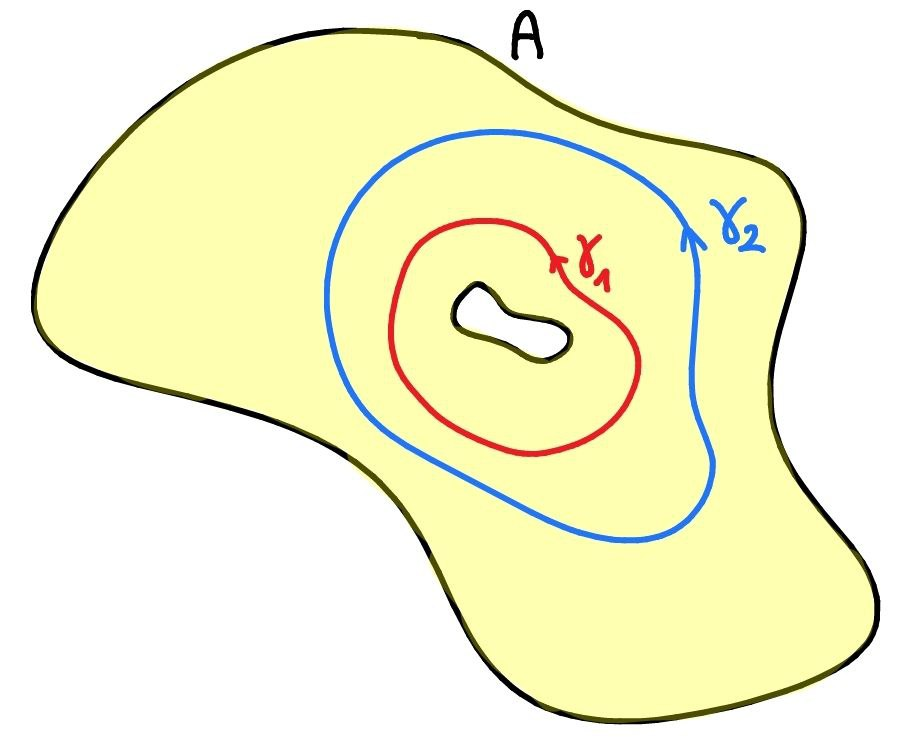
\includegraphics[width=4cm]{images/bonfa_2}
  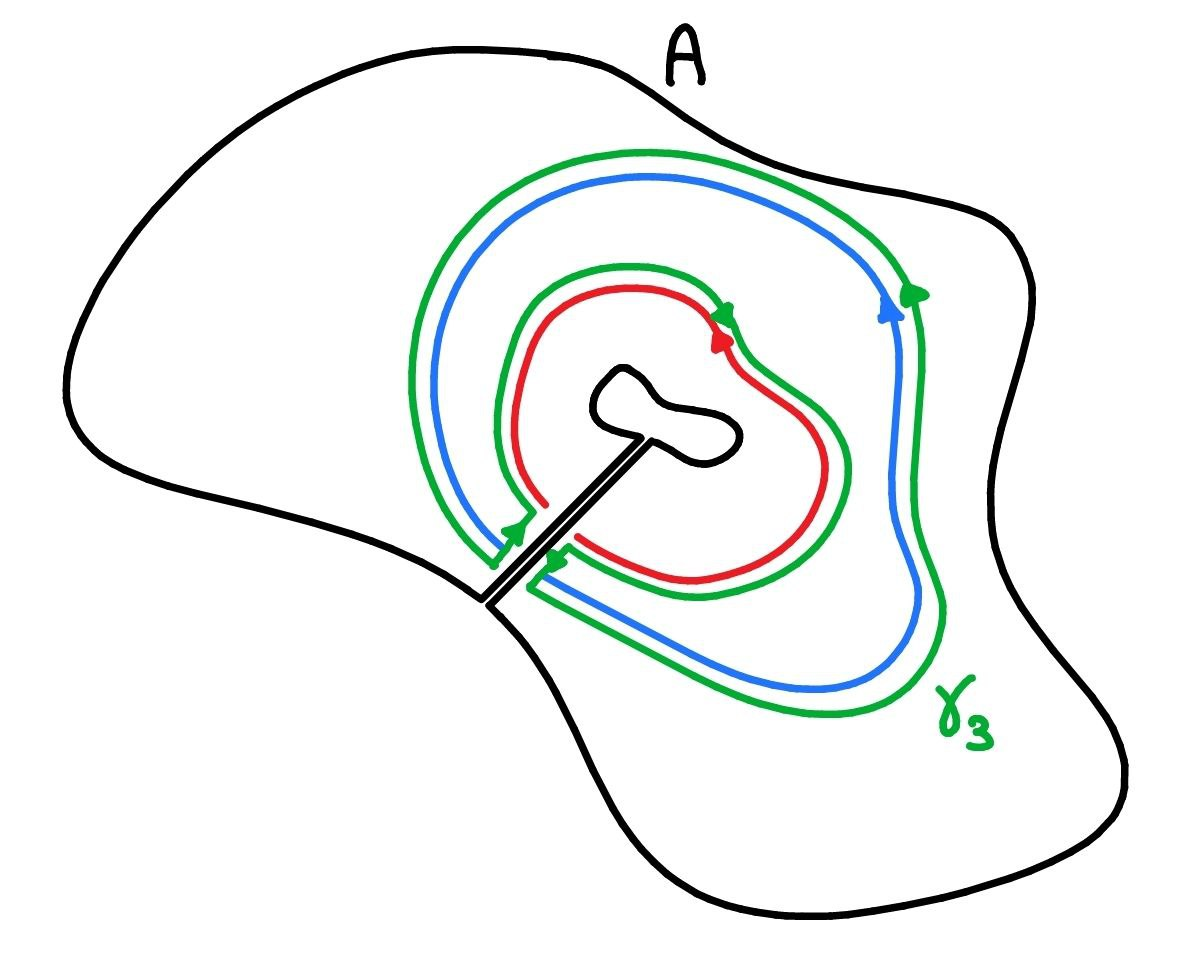
\includegraphics[width=4cm]{images/bonfa_3}
\end{center}
\end{figure}

Il teorema dell'integrale nullo si può estendere anche alla frontiera dell'aperto $A$, a patto che qui la funzione sia continua:
\begin{thm}
Siano $r$ curva semplice e chiusa (aka circuito), $A$ la regione aperta interna a $r$ (aka semplicemente connesso) e $f\in H(A)\cap\Cc^0(\overline{A})$. Allora $\int_r f(z)\dz=0$.
\end{thm}
\begin{proof}
Si basa sul deformare la funzione finché non si è raggiunta la frontiera $\partial A$, cioè la curva $r$.
\end{proof}

\section{Formula Integrale di Cauchy}

\begin{thm}
Sia $\gamma$ una curva semplice e chiusa, $A$ la sua regione interna e $f\in H(A) \cap \Cc^{0}(\overline{A})$. Allora $\forall z\in A$
\begin{equation*}
f(z) = \frac{1}{2\pi i}\int_{\gamma}\frac{f(w)}{w - z} \dw
\end{equation*}
\end{thm}

\begin{proof}
Fissiamo $z\in A$. La funzione $\dfrac{f(w)}{w - z}$ non è olomorfa in $A$, ma in $B=A\setminus\{z\}$. Tale $B$ non è più semplicemente connesso (ha un \textit{buco}) e dunque l'idea è quella di utilizzare la conseguenza del teorema dell'integrale nullo.

A tal proposito deformiamo $\gamma$ in una circonferenza $r$ centrata in $z$ di raggio $\rho$ opportuno (che non ci faccia uscire da $A$)
$$
r=z+\rho e^{it} \quad t\in[0,2\pi]
$$
in modo tale da poter riscrivere
\begin{equation*}
\int_{\gamma}\frac{f(w)}{w - z} \dw=\int_{r}\frac{f(w)}{w - z} \dw
\end{equation*}
Ora questo lo sappiamo calcolare, è un banale integrale di linea
\begin{equation*}
\int_{r}\frac{f(w)}{w - z} \dw = \int^{2\pi}_{0}\frac{f\left(z + \rho e^{it}\right)}{\cancel{\rho e^{it}}}\,\cancel{\rho e^{it}}i \dt = i\int^{2\pi}_{0} f\left(z + \rho e^{it}\right) \dt
\end{equation*}
Per la continuità di $f$ in $z$, e poichè $\left|e^{it}\right|=1$, otteniamo $f\left(z + \rho e^{it}\right)=f(z)+o(1)$ per $\rho\to 0$. Allora
\begin{equation*}
\int_{\gamma}\frac{f(w)}{w - z} \dw=\int_{r}\frac{f(w)}{w - z} \dw=i\int_{0}^{2\pi} \underbrace{f(z)}_{\text{cost}}\dt+i\int_0^{2\pi} \underbrace{o(1)}_{\to 0}\dt \xrightarrow[]{\rho\to 0} 2\pi i f(z)
\end{equation*}
\end{proof}

Questo è un teorema molto forte, in quanto conoscendo $f$ sul bordo, possiamo caratterizzare $f$ in ogni punto all'interno di $A$. Anzi, ci si può spingere ancora oltre: se due funzioni $f$ e $g$ olomorfe in $A$ e continue su $\partial A$ sono tali per cui $f(z)=g(z)$ per ogni $z\in\partial A$ allora sono uguali anche per ogni $z\in A$ (seconda conferma del fatto che le funzioni olomorfe hanno una struttura molto rigida).

\section{Esistenza di primitive}

Nei reali $f\in\Cc^0\ \Rightarrow\ \exists F$ primitiva tale che $F'(x)=f(x)$; invece nei complessi la continuità non è più condizione sufficiente per l'esistenza di una primitiva.
\begin{thm}
Sia $f:A\to\CC$ continua, $A$ aperto semplicemente connesso. Allora le seguenti affermazioni sono equivalenti:
\begin{enumerate}
    \item $\exists F:A\to\CC$ tale che $F'(z)=f(z)$ $\forall z\in A$
    \item $f\in H(A)$
    \item $u\,\de x-v\,\de y$ e $u\,\de y+v\,\de x$ sono forme differenziali esatte
\end{enumerate}
\end{thm}

\section{Serie di potenze}

Concludiamo la trattazione delle funzioni olomorfe con il \textit{Teorema di Weierstrass} (e relative conseguenze), grazie al quale avremo un'ultima conferma della rigidità delle funzioni olomorfe: se una funzione è derivabile in un aperto una volta allora è ivi derivabile infinite volte.

\begin{defn}
Una funzione è analitica in un aperto $A$ se ammette in ogni $z_0\in A$ un'espansione in serie di potenze.
\end{defn}

\begin{thm}[di Weierstrass]$\\$
Sia $f\in H(A)$, $A$ aperto. Allora $f$ è analitica, ovvero è rappresentabile nell'intorno di ogni punto $z_0\in A$ mediante la serie di potenze
\begin{equation*}
f(z) = \sum^{\infty}_{n = 0} a_{n}(z - z_{0})^{n}
\end{equation*}
dove 
\begin{equation*}
a_{n} = \frac{1}{2\pi i}\int_{\gamma}\frac{f(w)}{(w - z_{0})^{n + 1}} \dw \qquad \forall n\in \NN
\end{equation*}
e $\gamma$ è una qualsiasi circonferenza di centro $z_0$ e interna ad $A$.
\end{thm}

\begin{proof}
Per la formula di Cauchy
\begin{equation*}
f(z) = \frac{1}{2\pi i}\int_{\gamma}\frac{f(w)}{w - z} \dw
\end{equation*}
per ogni $z$ dentro il disco centrato in $z_0$ e con $w$ variabile di integrazione appartenente a $\gamma.$
\fg{0.4}{bonfa_4}
Osserviamo la figura risulta banale che
\begin{equation*}
\left| \frac{z - z_{0}}{w - z_{0}}\right| < 1
\end{equation*}
Possiamo usare tale formula per riscrivere la frazione $\dfrac{1}{w-z}$ che compare nella formula di Cauchy come somma di una serie geometrica:
$$
\frac{1}{w-z}=\frac{1}{w-z_0+z_0-z}=\frac{1}{w-z_0}\ \frac{1}{1-\frac{z-z_0}{w-z_0}}=\frac{1}{w-z_0}\sum_{n=0}^{\infty}\left(\frac{z-z_0}{w-z_0}\right)^n=\sum_{n=0}^{\infty}\frac{(z-z_0)^n}{(w-z_0)^{n+1}}
$$
Sostituendo nell'espressione di $f$ otteniamo
$$
f(z)=\frac{1}{2\pi i}\int_{\gamma}\frac{f(w)}{w-z}\dw=\frac{1}{2\pi i}\int_{\gamma}\left(f(w)\cdot \sum_{n=0}^{\infty}\frac{(z-z_0)^n}{(w-z_0)^{n+1}} \right)  \dw
$$
Ci ricordiamo che 
\begin{enumerate}
    \item una serie di potenze converge uniformemente strettamente all'interno del disco di convergenza
    \item su un intervallo limitato si può scambiare integrale e serie se la serie vi converge uniformemente
\end{enumerate}
Allora
$$
f(z)=\frac{1}{2\pi i}\int_{\gamma}\left(f(w)\cdot \sum_{n=0}^{\infty}\frac{(z-z_0)^n}{(w-z_0)^{n+1}} \right)  \dw=\frac{1}{2\pi i}\cdot \sum_{n=0}^\infty (z-z_0)^n \cdot \int_\gamma \frac{f(w)}{(w-z_0)^{n+1}}\dw
$$
Abbiamo dunque espresso una funzione olomorfa come serie di potenze, e in particolare abbiamo ottenuto
$$
f(z)=\sum_{n=0}^\infty a_n(z-z_0)^n \qquad a_n=\frac{1}{2\pi i}\int_{\gamma}\frac{f(w)}{(w-z_0)^{n+1}}\dw
$$
\end{proof}

\newpage

Conseguenze di tale teorema:
\begin{enumerate}
    \item [$\triangleright$] Presa una $f$ analitica, dato che si può esprimere localmente come serie di potenze per definizione, e che una serie di potenze è derivabile infinite volte, possiamo dire che $f$ analitica $\Rightarrow$ $f$ olomorfa.

    Invece grazie al teorema di Weierstrass abbiamo che $f$ olomorfa $\Rightarrow$ $f$ analitica.

    Mettendo insieme i due risultati abbiamo
    $$
    \boxed{f\text{ analitica }\Leftrightarrow\ f\text{ olomorfa}}
    $$

    \item [$\triangleright$] Sia $A$ un circuito e sia $f$ una funzione $f\in H(A)\cap\Cc^0(\overline{A})$. Allora
    \begin{equation*}
    f^{(n)}(z_{0}) = \frac{n!}{2\pi i}\int_{\partial A}\frac{f(w)}{(w - z_{0})^{n + 1}} \dw \qquad \forall z_0\in A,\ \forall n\in \NN
    \end{equation*}
    Tale formula è nota come \textbf{formula delle derivate}, ed è a tutti gli effetti una generalizzazione della fomrula integrale di Cauchy (caso $n=0$).
\end{enumerate}

Concludiamo il paragrafo con il
\begin{thm}[del massimo modulo]
Sia $A\subset\CC$ un aperto connesso e sia $f\in H(A)$. Se la funzione $z\mapsto |f(z)|$ assume in un punto di $A$ il suo valore massimo, allora $f$ è costante in $A$.
\end{thm}

\begin{coro}
Sia $A\subset\CC$ un aperto connesso e sia $f\in H(A)\cap\Cc^0(\overline{A})$. Se $f(z)\neq 0$ per ogni $z\in A$ allora la funzione $z\mapsto |f(z)|$ assume il suo valore minimo su $\partial A$.
\end{coro}

\section{Serie di Laurent}

Finora si è parlato di funzioni olomorfe, ora dobbiamo capire cosa succede nel caso di funzioni non olomorfe.

Abbiamo già incontrato delle funzioni che presentano dei punti \textit{critici}, per esempio il punto $z^*=1$ per la serie geometrica $f(z)=\frac{1}{1-z}$: essa ammette espansione in serie di Taylor centrata in $z_0=0$
\begin{equation*}
\sum_{n=0}^\infty z^n \qquad \text{ purché }|z|<1
\end{equation*}
Però la funzione $f$ è definita su tutto $\CC\setminus\{1\}$ e anzi è ivi olomorfa, quindi perché devo per forza centrare l'espansione in serie di potenze nell'origine? \\
Si dimostra che $f$ ammette espansione in serie di Taylor centrata in $z_0$
\begin{equation*}
\sum_{n=0}^\infty \frac{(z-z_0)^n}{(1-z_0)^{n+1}} \qquad \text{ purché }\left| \frac{z-z_0}{1-z_0} \right|<1\text{ cioè }|z-z_0|<|1-z_0|
\end{equation*} 
Possiamo quindi espandere la funzione $f$ in serie di Taylor in ogni direzione meno quella che include il punto critico $z^*=1$.

Punti $z^*$ che non permettono di scrivere un'espansione in serie di Taylor centrata in $z_0$ e il cui disco di convergenza li contenga, sono detti \textit{punti singolari}. Più precisamente:
\begin{defn}[Punto singolare]
Sia $f:A\to\CC$, $f\in H(A)$. Il punto $z^*\in\partial A$ è detto singolare per $f$ se non esiste una serie di potenze convergente anche in $z^*$.
\end{defn}

Come vedremo, queste singolarità sono di vario tipo e verranno opportunamente classificate.

Per risolvere il problema si introduce la \textit{serie di Laurent}, una \underline{serie di potenze bilatera} su una corona circolare $A$ (quindi \textit{non} semplicemente connessa) centrata nel punto stesso che compromette l'espansione in serie di Taylor.
\begin{thm}[Serie di Laurent]$\\$
Sia $A\subset\CC$ una corona circolare aperta, cioè costituita dai punti esterni a una circonferenza $\gamma_1$ e interni a una circonferenza $\gamma_2$, entrambe di centro $z_0$. Sia $f:A\to\CC$, $f\in H(A)$. Sia infine $\gamma$ una qualsiasi curva interna ad $A$ che concateni una volta $z_0$. Allora
\begin{equation*}
f(z) = \sum\limits^{\infty}_{n = - \infty} a_{n}(z - z_{0})^{n} \quad a_{n} = \frac{1}{2\pi i}\int_{\gamma}\frac{f(w)}{(w - z_{0})^{n + 1}} \dw \qquad \qquad \forall z\in A
\end{equation*}
\end{thm}

Osserviamo alcune cose:
\begin{enumerate}
    \item [(i)] La curva è \textit{qualsiasi} purché concateni $z_{0}$; ciò deriva dal fatto che la funzione è olomorfa nel dominio dove si esegue l'integrazione, e pertanto l'integrale non varia per deformazione continua.
    \item [(ii)] Sotto le ipotesi di tale teorema si riesce ad espandere $f$ come serie di potenze centrata non solo in un punto dove $f$ non è olomorfa, ma perfino in un punto dove $f$ non è nemmeno definita!
\end{enumerate}

Ma questo come ci aiuta?\\
Sia $f\in H(A\setminus\{z_0\})$, cioè $z_0$ è un punto singolare per $f$. Grazie al teorema di Laurent è possibile prendere una corona circolare di raggio interno piccolo a piacere e raggio esterno grande purché la corona rimanga all'interno di $A$, e scrivere $f$ come serie di Laurent centrata in $z_0$:

\begin{figure}[h!]
\begin{center}
  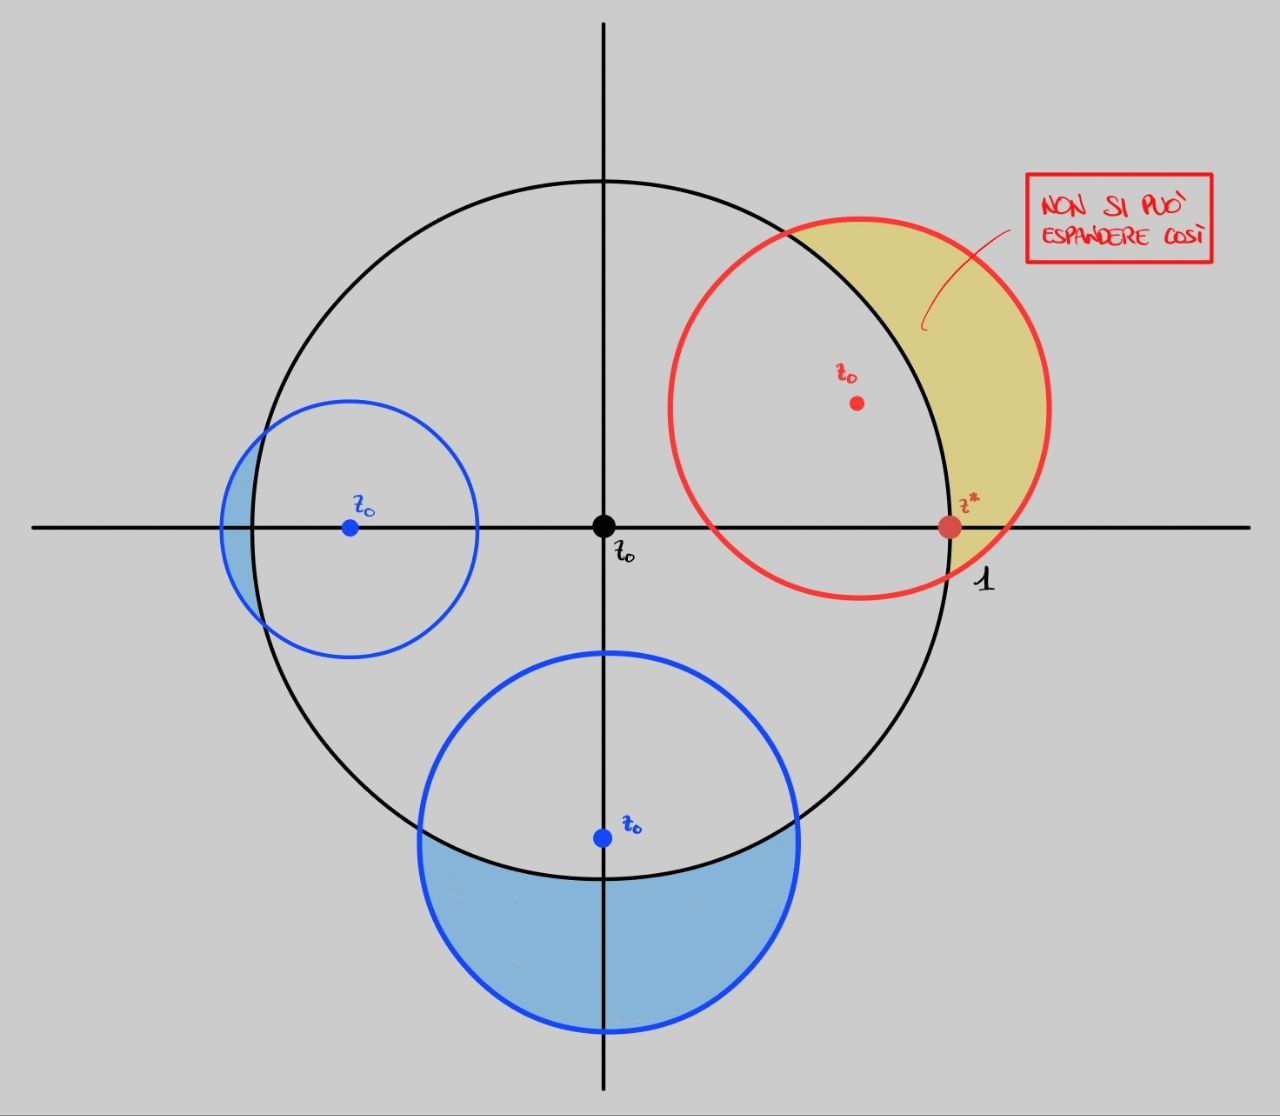
\includegraphics[width=6cm]{images/bonfa_6}
  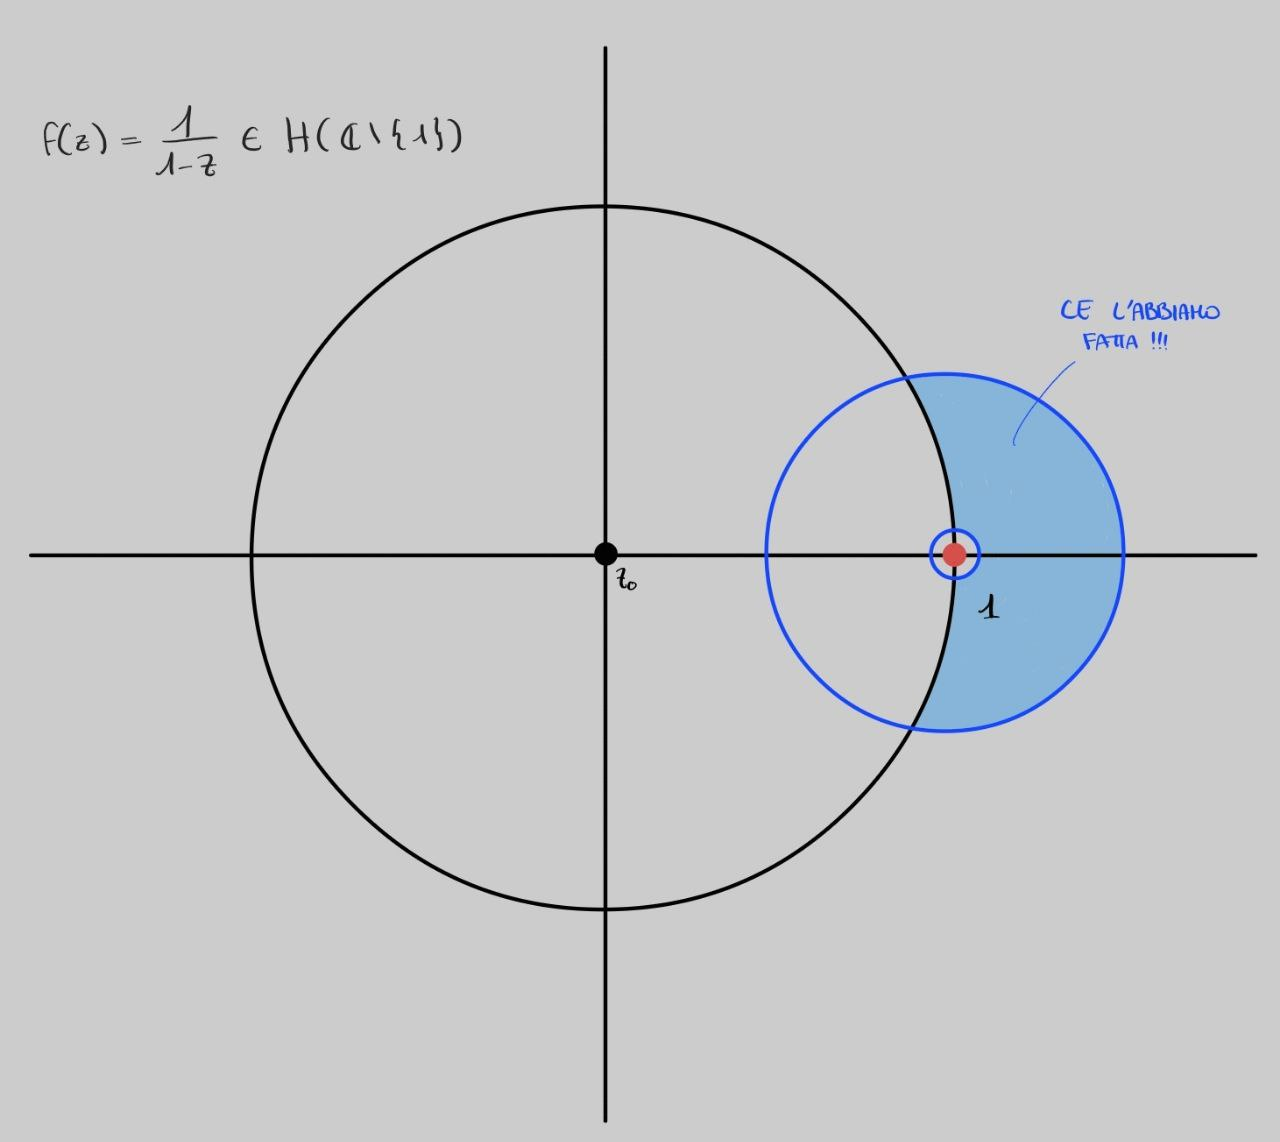
\includegraphics[width=6cm]{images/bonfa_7}
\end{center}
\end{figure}

\subsection{Classificazione delle singolarità al finito}

\begin{defn}[Punto singolare isolato]$\\$
Se $f\in H(d(z_0,r)\setminus\{z_0\})$ allora si dice che $z_{0}$ è un punto singolare isolato per $f$, e localmente si può scrivere tramite la serie di Laurent l'espansione $f(z)=\sum_{n=-\infty}^{+\infty}a_n(z-z_0)^n$.
\end{defn}

Una singolarità isolata può essere di tre tipi:
\begin{enumerate}
    \item [$\triangleright$] singolarità eliminabile se $\lim_{z\to z_0}f(z)$ esiste finito.
    \item [$\triangleright$] polo se $\lim_{z\to z_0}f(z)=\infty$.
    \item [$\triangleright$] singolarità essenziale se $\not\exists\lim_{z\to z_0}f(z)$.
\end{enumerate}

\textit{Esempio}. Consideriamo le seguenti funzioni:\leavevmode
\begin{equation*}
f(z)=\frac{\sin z}{z} \qquad g(z)=\frac{1}{1-z} \qquad h(z)=\begin{cases}
e^{1/z} \\ \sin\frac{1}{z} \\ \cos\frac{1}{z}
\end{cases}
\end{equation*}
Possiamo dire che:
\begin{itemize}
    \item $f$ ha una singolarità eliminabile in $z=0$ poiché
    \begin{equation*}
    f(z) = \frac{\sin z}{z} = \frac{1}{\cancel{z}}\sum\limits^{\infty}_{n = 0}\frac{(- 1)^{n} z^{2n+\cancel{1}}}{(2n + 1) !} = \sum\limits^{\infty}_{n = 0}\frac{(- 1)^{n} z^{2n}}{(2n + 1) !}
    \end{equation*}
    e dunque sebbene $f$ sia definita su $\CC\setminus\{0\}$, è olomorfa su tutto $\CC$.
    \item $g$ ha un polo in $z=1$.
    \item $h$ ha una singolarità essenziale in $z=0$.
\end{itemize}

Alla luce del teorema di Laurent, possiamo scomporre l'espansione di $f$ in
\begin{equation*}
f(z)=\sum_{n \in \mathbb{Z}} a_n\left(z-z_0\right)^n=\sum_{n=0}^{+\infty} a_n\left(z-z_0\right)^n+\sum_{n=-\infty}^{-1} a_n\left(z-z_0\right)^n
\end{equation*}
dove la serie di potenze con indici negativi è proprio la parte che descrive il comportamento \textit{singolare} della funzione.

Allora introduciamo
\begin{defn}
$M=\left\{n\in\ZZ\ :\ a_n\neq 0,\ n<0 \right\}$ è detto insieme degli indici della parte singolare dello sviluppo di Laurent.
\end{defn}
in modo tale da poter caratterizzare le singolarità di una funzione attraverso:
\begin{enumerate}
    \item [$\triangleright$] singolarità eliminabile se e solo se $M=\varnothing$, cioè gli $a_n$ con $n$ negativo sono tutti nulli.
    \item [$\triangleright$] polo se e solo se $0<|M|<+\infty$, cioè è nullo solo un numero finito di $a_n$ con $n$ negativo; in particolare il polo è di ordine $m$, essendo $m$ il più grande intero positivo per il quale $a_{-m}\neq 0$.
    \item [$\triangleright$] singolarità essenziale se $|M|=+\infty$, cioè esistono infiniti $a_n$.
\end{enumerate}

Per quanto riguarda l'ordine dei poli, nella pratica è tutto più semplice: 
\begin{equation*}
f(z)=\frac{e^{\frac{1}{z-1}}}{z^2(z^2+4)}\ :\ 0\text{ è un 2-polo, }\pm 2i\text{ sono entrambi 1-poli}
\end{equation*}

Concludiamo con due teoremi:
\begin{thm}
[Caratterizzazione delle singolarità essenziali] Sia $z_{0}$ una singolarità essenziale isolata per $f(z)$. Allora la funzione $\frac{1}{f(z)}$ ha in $z_{0}$ una singolarità essenziale oppure un punto di accumulazione di poli.
\end{thm}

\textit{Esempi.}\leavevmode
\begin{align*}
\sin\frac{1}{z}\text{ ha s. essenz. in }z=0 \  &\longrightarrow\ \frac{1}{\sin\frac{1}{z}}\text{ è pt. di accumulo di s. in }z=0 \\
e^{\frac{1}{z}}\text{ ha s. essenz. in }z=0 \  &\longrightarrow\  \frac{1}{e^{1/z}}\text{ ha s. essenz. in }z=0
\end{align*}

\begin{thm}[di Picard]
Sia $f$ una funzione olomorfa che ha singolarità essenziale in $z_0$. Allora in qualsiasi intorno di $z_0$ ($z_0$ escluso) la funzione assume tutti, al più uno, i valori complessi inifite volte.
\end{thm}

Riusciamo così ad intuire le infinite problematiche legate alle singolarità essenziali.

\subsection{Classificazione delle singolarità all'infinito}

In $\CC$ non ha senso parlare di $\pm \infty $, essendoci infinite direzioni, tuttavia è utile considerare tutti i punti infinitamente distanti \textit{come un unico punto all'infinito}; più nello specifico vale la seguente definizione.
\begin{defn}
[Punto singolare all'infinito] Il punto all'infinito $z_{\infty}$ è singolare per $f(z)$ se $z_{0} = 0$ è singolare per $f\left(\frac{1}{z}\right)$.
\end{defn}

\begin{defn}
[Punto singolare isolato all'infinito] Il punto all'infinito $z_{\infty}$ è isolato per $f(z)$ se è singolare e tutti i punti singolari al finito per $f$ ricadono all'interno di un disco di raggio $R$, cioè $f\in H(\{|z|>R\})$.
\end{defn}

Dunque per $f$ si ha che $\infty$ è:
\begin{enumerate}
    \item [$\triangleright$] singolarità eliminabile se $\lim_{z\to \infty}f(z)$ esiste finito.
    \item [$\triangleright$] polo se $\lim_{z\to \infty}f(z)=\infty$.
    \item [$\triangleright$] singolarità essenziale se $\not\exists\lim_{z\to \infty}f(z)$.
\end{enumerate}

Segnaliamo che se $f(z)\sim\dfrac{1}{z^{\alpha}}$ allora il punto $z=\infty$ è singolarità eliminabile, e in particolare è uno zero di ordine $\alpha$.

Analogamente al caso finito, definito $M=\left\{n\in\ZZ\ :\ a_n\neq 0,\ n>0 \right\}$ si ha che
\begin{enumerate}
    \item [$\triangleright$] singolarità eliminabile se e solo se $M=\varnothing$.
    \item [$\triangleright$] polo se e solo se $0<|M|<+\infty$; in particolare il polo è di ordine $m$, essendo $m$ il più grande intero positivo per il quale $a_{m}\neq 0$.
    \item [$\triangleright$] singolarità essenziale se e solo se $|M|=\infty$.
\end{enumerate}

Per quanto riguarda l'ordine dei poli, nella pratica è tutto più semplice: 
\begin{equation*}
f(z)=\frac{z^5}{(1+iz)^2}\ :\ \infty\text{ è un 3-polo}
\end{equation*}

Vi è inoltre un terzo modo per studiare la singolarità all'infinito: $\infty$ è punto di singolarità eliminabile, polo, singolarità essenziale per $f(z)$ se 0 è punto di singolarità eliminabile, polo, singolarità essenziale per $g(z)=f(1/z)$.

\textit{Esempio.}\\
La funzione $f(z) = e^{z}$ ha singolarità isolata essenziale all'infinito, mentre $g(z) = \frac{1}{\sin z}$ ha punto all'infinito non isolato.

\begin{rem}
Al variare dell'aperto $A$ considerato, può variare la serie di Laurent associata ad una funzione $f$: in altre parole, bisognerà volta per volta precisare in quale corona si andrà ad operare. A titolo di esempio, prendiamo la funzione $f(z)=\dfrac{1}{z(1-z)}$; risulta
\begin{align*}
\text{nella corona }0<|z|<1\text{ centrata in }z_0=0 \qquad f(z)&=\sum_{n=-1}^{+\infty} z^n \\
\text{nella corona }0<|z-1|<1\text{ centrata in }z_0=1 \qquad f(z)&=\sum_{n=-1}^{+\infty}(-1)^n(z-1)^n \\
\text{nella corona }1<|z|\text{ centrata in }z_0=\infty \qquad f(z)&=-\sum_{n=-\infty}^{-2}z^n
\end{align*}
Dunque in 0 e 1 ci sono dei poli, all'infinito una singolarità eliminabile.
\end{rem}

\newpage

\section{Teorema dei residui}

Riprendiamo l'espansione in serie di Laurent 
\begin{equation*}
f(z) = \sum\limits^{\infty}_{n = - \infty} a_{n}(z - z_{0})^{n} \quad a_{n} = \frac{1}{2\pi i}\int_{\gamma}\frac{f(w)}{(w - z_{0})^{n + 1}} \dw
\end{equation*}
Osserviamo che per $n=-1$ il denominatore $(w - z_{0})^{n + 1}$ si annulla, e rimane
\begin{equation*}
a_{- 1} = \frac{1}{2\pi i}\int_{\gamma} f(w) \dw
\end{equation*}
Allora
\begin{defn}
Si dice residuo di $f$ in $z_0$ la quantità $\Res(f,z_0):=a_{-1}$.
\end{defn}
In questo modo possiamo caratterizzare l'integrale curvilineo di $f$:
\begin{equation*}
\boxed{\int_{\gamma} f(w) \dw=2\pi i\cdot \Res(f,z_0)}
\end{equation*}

Ma per cosa sta l'aggettivo ``residuo''?\\
Per il teorema dell'integrale nullo di Cauchy, su un insieme semplicemente connesso si ha $\int_{\gamma} f(w) \dw=0$; invece su un insieme non semplicemente connesso l'integrale non è nullo, proprio perché la funzione lascia un \textit{residuo}.

\begin{thm}[dei Residui]$\\$
Sia $A$ semplicemente connesso. Sia $f\in H(A\setminus \{z_{1}, \dotsc, z_{n}\})$, dunque $z_1,\dotsc,z_n$ sono punti singolari e $f$ è olomorfa su un insieme non più semplicemente connesso. Allora
\begin{equation*}
\int_{\gamma} f(z) \dz = 2\pi i \cdot \sum\limits^{n}_{k = 1}\Res (f, z_{k})
\end{equation*}
\end{thm}

\begin{proof} 
Vediamo una dimostrazione abbastanza approssimativa e per $k=2$; la situazione è questa:

\fg{0.3}{bonfa_8}

Vogliamo calcolare $\int_{\gamma}f(z)\dz$, ma per ora sappiamo dalla definizione di residuo che
$$\int_{\Gamma_1}f(z)\dz=2\pi i\cdot \Res(f,z_1) \qquad \int_{\Gamma_2}f(z)\dz=2\pi i\cdot \Res(f,z_2)$$
Per sbloccare la situazione usiamo la conseguenza del teorema dell'integrale nullo di Cauchy deformando con continuità $\gamma$ in $\gamma'$ \textit{girando attorno} alle singolarità:

\fg{0.3}{bonfa_9}

Da una parte 
$$\int_{\gamma'}f(z)\dz=0$$
perché $\gamma'$ ora racchiude un insieme \textit{senza buchi}; dall'altra, per l'additività dell'integrale 
$$
\int_{\gamma'}f(z)\dz=\int_\gamma f(z)\dz+\int_{\Gamma_1}f(z)\dz+\int_{\Gamma_2}f(z)\dz
$$
Mettendo a sistema le due cose otteniamo
\begin{equation*}
\int_\gamma f(z)\dz=-\int_{\Gamma_1}f(z)\dz-\int_{\Gamma_2}f(z)\dz=-2\pi i\left(\Res(f,z_1)+\Res(f,z_2)\right)
\end{equation*}
che è quanto volevasi dimostrare.
\end{proof}

\textit{Esempio.}\\
La funzione geometrica $f(z)=\frac{1}{1-z}$ ha $z^*=1$ come punto singolare. Si calcola facilmente $\Res(f,z^*)$, in quanto la funzione è già scritta in serie di Laurent: $f(z)=-(z-1)^{-1}$ e quindi $\Res(f,z^*)=a_{-1}=-1$.

\begin{defn}
Si dice residuo di $f$ in $\infty$ la quantità $\Res(f,\infty):=-a_{-1}$.
\end{defn}

\begin{thm}
Sia $f\in H(\CC\setminus\{z_1,\dotsc,z_n\})$. Allora
\begin{equation*}
\sum\limits^{n}_{k = 1}\Res (f, z_{k}) + \Res (f, \infty) = 0
\end{equation*}
\end{thm}

\begin{proof}
Prendiamo la circonferenza $r:[0,2\pi]\to\CC$ parametrizzata da $r(t)=Re^{it}$ che contiene tutti i punti $z_1,\dotsc,z_n$. 

Da una parte, per definizione, abbiamo
\begin{align*}
\int_r f(z)\dz&:=\int_0^{2\pi} f(Re^{it})\cdot Rie^{it}\dt =\\
&=\int_0^{2\pi} \sum_{n\in\ZZ} a_n R^ne^{int}Rie^{it}\dt =\\
&=i\sum_{n\in\ZZ}a_nR^{n+1}\underbrace{\int_0^{2\pi}e^{i(n+1)t}\dt}_{\neq 0\Leftrightarrow n=-1} =\\
&=2\pi i \cdot a_{-1} =\\
&=-2\pi i\cdot \Res(f,\infty)
\end{align*}
Dall'altra, per il teorema dei residui, abbiamo
\begin{equation*}
\int_r f(z)\dz=2\pi i\cdot \sum_k\Res(f,z_k)
\end{equation*}
Mettendo a sistema i due risultati si ottiene la tesi
$$
\sum\limits^{n}_{k = 1}\Res (f, z_{k}) = - \Res (f, \infty)
$$
\end{proof}

\section{Calcolo dei residui}

Nei punti $z_{0} \neq \infty $
\begin{enumerate}
\item se è una singolarità eliminabile:
\begin{equation*}
\Res \left(f, z_{0}\right) = 0
\end{equation*}
\item se è un polo
\begin{enumerate}
\item semplice (di ordine $p = 1$)
\begin{equation*}
\Res \left(f, z_{0}\right) = \lim\limits_{z\rightarrow z_{0}} f(z)\left(z - z_{0}\right)
\end{equation*}
\item di ordine $p \geq 2$
\begin{equation*}
\Res \left(f, z_{0}\right) = \frac{1}{\left(p - 1\right) !}\lim\limits_{z\rightarrow z_{0}}\left\{\frac{d^{p - 1}}{dz^{p - 1}}\left[ f(z)\left(z - z_{0}\right)^{p}\right]\right\}
\end{equation*}
\end{enumerate}
\item se è una singolarità essenziale bisogna per forza fare lo sviluppo di Laurent (che è valido in tutti i casi in realtà, ma è decisamente più laborioso la maggior parte delle volte)
\end{enumerate}

In alternativa, con una funzione del tipo $F = \frac{f}{g}$, se $f\in \Hc \left(\Uc \left(z_{0}\right)\right)$ e $g$ ha in $z_{0}$ uno zero semplice ($g\left(z_{0}\right) = 0$ e $g'\left(z_{0}\right) \neq 0$), allora
\begin{equation*}
\Res \left(\frac{f}{g}, z_{0}\right) = \frac{f\left(z_{0}\right)}{g'\left(z_{0}\right)}
\end{equation*}
Ricordiamo che se $f$ non si annulla in $z_{0}$ allora $F$ ha in $z_{0}$ un polo del I ordine. Se $f$ si annulla in $z_{0}$ allora $F$ ha in $z_{0}$ una singolarità eliminabile.

Invece per $z_{0} = \infty $:
\begin{enumerate}
\item $\Res (f, \infty) = \Res \left(- \frac{1}{z^{2}} f\left(\frac{1}{z}\right), 0\right)$
\item se è zero di ordine $1$ allora $\Res (f, \infty) = - \lim\limits_{z\rightarrow \infty} zf(z)$
\item se è zero di ordine $ \geq 2$ allora $\Res (f, \infty) = 0$
\end{enumerate}


\section{Lemmi di Jordan}

In questo paragrafo vediamo alcuni lemmi che consentono il calcolo di integrali di linea mediante opportuni passaggi al limite: le loro principali applicazioni sono nel calcolo delle trasformate di Fourier e delle antitrasformate di Laplace.

Consideriamo un generico arco di circonferenza:
\begin{equation*}
C_{R}(t_{1}, t_{2}) = \left\{z\in \CC : z = Re^{it}, t \in [t_{1}, t_{2}]\right\}
\end{equation*}

\begin{lemma}
Sia $f(z)$ continua su $C_{R}$. Allora
\begin{equation*}
\left| \int_{C_{R}} f(z)\dz\right| \leq R(t_{2} - t_{1})\cdot \max_{t\in [t_1,t_2]}\left|f(Re^{it})  \right|
\end{equation*}
dove $R(t_{2} - t_{1})$ non è altro che la lunghezza dell'arco considerato.
\end{lemma}

\begin{coro}[per il cerchio grande]
Se $\exists b>1$ tale che $|f(z)| \leq \dfrac{k}{|z|^{b}}$ per ogni $z$ tale che $|z|\geq R_0$ allora
\begin{equation*}
\lim_{R\rightarrow +\infty}\ \int_{C_{R}} f(z)\dz = 0
\end{equation*}
\end{coro}

\begin{coro}[per il cerchio piccolo]
Sia $f\in H(d(z_0,r)\setminus\{z_0\})$ con $z_0$ 1-polo per $f$; sia $C_{\varepsilon}(t)=z_0+\varepsilon e^{it}$ con $t\in[t_1,t_2]$. Allora
\begin{equation*}
\lim_{\varepsilon\rightarrow 0^+}\ \int_{C_{\varepsilon}} f(z)\dz = (t_2-t_1)\,i\cdot\Res(f,z_0) 
\end{equation*}
\end{coro}

Per concludere vediamo un risultato generale più mirato al calcolo di serie di Fourier.

\begin{lemma}[di Jordan]
Sia $f:A\to\CC$ continua su $C_R(0,\pi)$ e sia $\omega>0$. Allora
\begin{equation*}
\left| \int_{C_R} e^{i\omega z}f(z)\dz \right| \leq K\cdot \max_{t\in[0,\pi]}\left|f(Re^{it})\right|
\end{equation*}
e $K$ non dipende da $R$.
\end{lemma}

\fg{0.4}{bonfa_10}

\begin{proof}\leavevmode
\begin{equation*}
\begin{aligned}
\left|\int_{C_R} e^{i \omega t} f(z) \dz\right| &\stackrel{\mathrm{DEF}}{=}\left|\int_0^\pi e^{i \omega(\cos t+i \sin t) R} f\left(R e^{i t}\right) \cdot R \cancel{i e^{i t}} \dt\right|\\
&\leqslant \underbrace{\max _{t \in[0, \pi]}\left|f\left(R e^{i t}\right)\right|}_M\cdot\left|\int_0^\pi Re^{i \omega(\cos t+i \sin t) R} \dt\right|\\
&=M\left|\int_0^\pi R\ \cancel{e^{\text {Ri}\omega \cos t}}\ e^{-R \omega \sin t} \dt\right|\\
&=2 M\left|\int_0^{\pi / 2} R e^{-\omega R \sin t} \dt\right|\\
&\leqslant 2 M\left|\int_0^{\pi / 2} R e^{-\omega R t} \dt\right| \qquad \left(\sin x\leq x\text{ se } x\in[0,\pi/2]\right)\\
&=2 M \cancel{R}\left|\left[\frac{1}{-\omega \cancel{R}}\ e^{-\omega R t}\right]_0^{\pi / 2}\right|\\
&\leqslant \frac{2 M}{\omega}\left|e^{-\omega R \pi / 2}-1\right|\\
&\leqslant \frac{2 M}{\omega}\\
&=K M \text { con } k=\frac{2}{\omega}
\end{aligned}
\end{equation*}
\end{proof}

\newpage

Come corollari di ciò ci sono i casi in cui si ha
\begin{itemize}
    \item $\displaystyle\int_{C_R} e^{i\omega z}f(z)\dz$ ma $\omega<0$: si prende
    \fg{0.4}{bonfa_11}

    \item $\displaystyle\int_{C_R} e^{\omega z}f(z)\dz$ con $\omega>0$ o $\omega<0$: si prendono rispettivamente
    \begin{figure}[h!]
    \begin{center}
      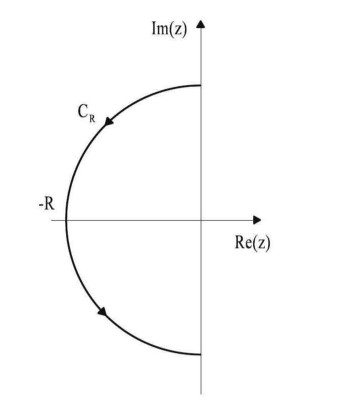
\includegraphics[width=4cm]{images/bonfa_12}
      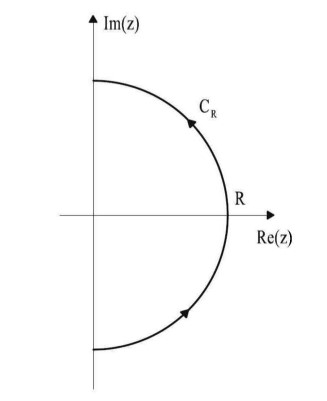
\includegraphics[width=4cm]{images/bonfa_13}
    \end{center}
    \end{figure}
\end{itemize}


\chapter{Spazi di Banach e Spazi di Hilbert}

Addentriamoci nell'\textit{Analisi funzionale} parlando di \textbf{spazi funzionali}.

\section{Spazi vettoriali e norme}

Iniziamo con un elenco delle nozioni basilari dell'algebra lineare.

\begin{defn}[Spazio vettoriale]
Sia $\KK$ il campo dei reali o dei complessi. Gli elementi di $\KK$ verranno detti scalari. Uno spazio vettoriale (o lineare) sul campo $\KK$ è un insieme non vuoto $X$ tale che:
\begin{enumerate}
    \item [(i)] per ogni coppia di elementi $x,y\in X$ esista un terzo elemento di $X$ che indicheremo con $x+y$
    \item [(ii)] per ogni $x\in X$ e $\lambda \in \KK$ esista un elemento di $X$ che indicheremo con $\lambda x$
\end{enumerate}
Tali operazioni di sommma e prodotto devono soddisfare le seguenti proprietà:
\begin{enumerate}
    \item [$\diamond$] per ogni $x,y,z\in X$ si ha $(x+y)+z=x+(y+z)$
    \item [$\diamond$] per ogni $x\in X$ esiste l'elemento nullo $0\in X$ tale che $0+x=x+0=x$
    \item [$\diamond$] per ogni $x\in X$ esiste l'elemento opposto $-x\in X$ tale che $x+(-x)=(-x+x)=0$
    \item [$\diamond$] per ogni $x,y\in X$ si ha $x+y=y+x$
    \item [$\diamond$] per ogni $x,y\in X$ e per ogni $\lambda\in\KK$ si ha $\lambda(x+y)=\lambda x+\lambda y$
    \item [$\diamond$] per ogni $x\in X$ e per ogni $\lambda,\mu\in\KK$ si ha $(\lambda+\mu)x=\lambda x +\mu x$
    \item [$\diamond$] per ogni $x\in X$ e per ogni $\lambda,\mu\in\KK$ si ha $(\lambda \mu)x=\lambda(\mu x)$
    \item [$\diamond$] per ogni $x\in X$ si ha $1x=x$
\end{enumerate}
\end{defn}

\begin{defn}[Sottospazio vettoriale]
Sia $X$ uno spazio vettoriale. Un sottoinsieme non vuoto $Y$ di $X$ si dice sottospazio vettoriale di $X$ se:
\begin{enumerate}
    \item [(i)] per ogni $x,y\in Y$ si ha $x+y\in Y$
    \item [(ii)] per ogni $x\in Y$ e per ogni $\lambda\in\KK$ si ha $\lambda x\in Y$
\end{enumerate}
\end{defn}
In altre parole $Y$ è a sua volta uno spazio vettoriale con le operazioni di somma e prodotto indotte da $X$ stesso.

\begin{defn}[Combinazione lineare]
Sia $X$ uno spazio vettoriale. Dati $n$ vettori $x_1,\dots,x_n\in X$ si chiama combinazione lineare di $x_1,\dots,x_n$ a coefficienti $\lambda_1,\dots,\lambda_n\in\KK$ la seguente somma
\begin{equation*}
\sum_{k=1}^n \lambda_kx_k
\end{equation*}
\end{defn}

\begin{defn}
Sia $X$ uno spazio vettoriale. I vettori $x_1,\dots,x_n\in X$ si dicono linearmente indipendenti se dati $\lambda_1,\dots,\lambda_n\in\KK$ tali che
\begin{equation*}
\sum_{k=1}^n \lambda_kx_k=0
\end{equation*}
si ha necessariamente che $\lambda_1=\cdots=\lambda_n=0$.
\end{defn}

\begin{defn}
Sia $X$ uno spazio vettoriale. Dati $n$ vettori $x_1,\dots,x_n\in X$ si dice che essi generano $X$ se per ogni $x\in X$ esistono $\lambda_1,\dots,\lambda_n\in\KK$ tali che
\begin{equation*}
x=\sum_{k=1}^n \lambda_kx_k
\end{equation*}
In tal caso si scrive $X=\text{span}\{x_1,\dots,x_n\}$. 

Se inoltre i vettori $x_1,\dots,x_n$ sono linearmente indipendenti allora si dice che l'insieme $\{x_1,\dots,x_n\}$ forma una base di $X$.
\end{defn}

\begin{defn}[Dimensione]
Sia $X$ uno spazio vettoriale che ammette una base di $n$ vettori. Allora si dice che $X$ ha dimensione $n$, e si pone $\dim X=n$. Se $X$ non ammette alcuna base formata da un numero finito di vettori, allora $\dim X=\infty$.
\end{defn}

\begin{thm}
La dimensione di uno spazio vettoriale non dipende dalla base scelta.
\end{thm}

\textit{Esempio.}

Consideriamo lo spazio $\KK$ delle $n$-uple ordinate di numeri reali o complessi. Definendo la somma di vettori come
$$
(x_1,\ddots,x_n)+(y_1,\dots,y_n):=(x_1+y_1,\dots,x_n+y_n)
$$
e il prodotto tra scalare e vettore come
$$
\lambda(x_1,\dots,x_n):=(\lambda x_1,\dots, \lambda x_n)
$$
si ottiene lo spazio vettoriale $\KK^n$ su $\KK$ e risulta $\dim \KK^n=n$. Si osservi che lo spazio vettoriale $\CC^n$ su $\CC$ può anche essere considerato come spazio vettoriale sul campo $\RR$, ma in questo caso $\dim \CC^n=2n$. 

\begin{defn}
[Norma]
Sia $X$ uno spazio vettoriale (qualsiasi, ovvero sia reale che complesso, sia di dimensione finita che infinita). Si dice norma un'applicazione $ \Vert \cdot \Vert : X\rightarrow [0, + \infty)$ che verifica
\begin{itemize}
\item $ \Vert x \Vert = 0\iff x = 0$ (annullamento)
\item $ \Vert \lambda x \Vert = | \lambda |\, \Vert x \Vert $ (omogeneità)
\item $ \Vert x + y \Vert \leq \Vert x \Vert + \Vert y \Vert $ (disuguaglianza triangolare)
\end{itemize}
$\forall \lambda \in \RR$, $\forall x, y\in X$
\end{defn}

\textit{Esempio.}\\
Dato lo spazio vettoriale $\RR^n$ (dim finita) l'applicazione $ \Vert \cdot \Vert : \RR^{n}\rightarrow [0, + \infty)$, $1 \leq p < + \infty $, definita da
\begin{equation*}
\Vert x \Vert_{p} = \left(\sum_{k=1}^n|x_k|^p\right)^{1/p}
\end{equation*}
è la norma $p$. Si noti che per $n=1$ coincide con il valore assoluto, per $p=2$ si ottiene la norma euclidea
\begin{equation*}
\Vert x \Vert_{2} = \sqrt{\sum_{k=1}^n x_k^2}
\end{equation*}
mentre per $p=\infty$ la norma infinito
\begin{equation*}
\Vert x \Vert_{\infty} = \max_k |x_k|
\end{equation*}

\textit{Esempio.}\\
Dato lo spazio vettoriale delle funzioni $\Cc^0\left([a,b]\right)$ (dim infinita), $a,b\in\RR$, si definisce norma $p$, $1 \leq p < + \infty $, la funzione
\begin{equation*}
\Vert f \Vert_{p}=\int_a^b |f(x)|^p \dx
\end{equation*}
In particolare per $p=\infty$ si ottiene la norma infinito o uniforme
\begin{equation*}
\Vert f \Vert_{\infty}=\max_{x\in[a,b]}|f(x)|
\end{equation*}

\begin{defn}
[Spazio normato]
Uno spazio vettoriale dotato di norma si dice spazio normato.
\end{defn}

\begin{defn}
[Metrica]
La funzione 
\begin{align*}
d: X\times X&\rightarrow [0, + \infty) \\
(x,y)&\mapsto d(x,y)=\Vert x-y\Vert
\end{align*}
è detta metrica, o distanza, indotta dalla norma.
\end{defn}
Dunque la norma misura un singolo elemente, la metrica misura la distanza fra due elementi dello spazio.

\begin{rem}
La distanza rispetta le seguenti proprietà:
\begin{enumerate}
    \item [(i)] $d(x,y)=0\ \Leftrightarrow\ x=y$
    \item [(ii)] $d(x,y)=d(y,x)$
    \item [(iii)] $d(x,z)\leq d(x,y)+d(y,z)$
\end{enumerate}
pertanto possiamo intuire che essa può essere introdotta su qualsiasi insieme, non necessariamente su uno spazio vettoriale (al contrario della norma, che ha senso solo su uno spazio vettoriale); inoltre possiamo introdurre una distanza su uno spazio vettoriale che non induce alcuna norma.

Capiamo quindi che il concetto di metrica è molto più generale del concetto di norma, ma per quanto verrà fatto in questo corso i due oggetti coincideranno.
\end{rem}

\begin{defn}
[Spazio metrico]
Uno spazio normato dotato di metrica si dice spazio metrico.
\end{defn}

\begin{thm}
Uno spazio normato è uno spazio metrico.
\end{thm}

È pertanto possibile introdurre sugli spazi normati tutte nozioni di carattere topologico quali ad esempio i concetti di insieme aperto e chiuso, contiinuità di funzioni, convergenza di successioni, etc. Riportiamo qui sotto la definizione di coonvergenza di una successione.

\begin{defn}[Successione convergente]
Sia $X$ uno spazio vettoriale normato. Una successione $\{x_n\}\subset X$ si dice convergente a $x\in X$ se $d(x_n,x)=\Vert x_n-x\Vert\to 0$ per $n\to\infty$.
\end{defn}

\newpage

\section{Spazi di Banach}

La nozione di completezza di uno spazio è legata al comportamento di particolari successioni che definiamo come segue:

\begin{defn}
[Successione di Cauchy]
Sia $X$ uno spazio normato. Una successione $\{x_{n}\}\subset X$ è di Cauchy se
\begin{equation*}
\forall \varepsilon > 0\ \ \exists N\in\NN\ \ \text{ t.c. }\ \ \Vert x_{n} - x_{m} \Vert < \varepsilon\ \ \forall n,m>N
\end{equation*}
\end{defn}
In altre parole le successioni di Cauchy ``non divergono nè oscillano''. Infatti le successioni convergenti sono successioni di Cauchy. Tuttavia, il viceversa non vale, ovvero possono esistere successioni di Cauchy che non convergono, ma che nè divergono nè oscillano. Pertanto ha senso la seguente definizione:
\begin{defn}
[Spazio completo]
Uno spazio normato si dice completo se ogni successione di Cauchy è convergente.
\end{defn}

\begin{defn}
[Spazio di Banach]
Uno spazio normato si dice di Banach se è completo rispetto alla metrica indotta dalla norma.
\end{defn}

\begin{rem}
Uno spazio di Banach può avere dimensione sia finita che infinita, anzi in questo capitolo è proprio quest'ultimo caso che ci interessa: vogliamo estendere i concetti di algebra visti nei precedenti corsi al caso di spazi vettoriali $\infty$-dimensionali. 

Infatti sappiamo che uno spazio vettoriale a dimensione finita è banalmente completo, ovvero di Banach.
\end{rem}

\textit{Esempio.}\\
L'insieme dei numeri razionali $\QQ$ non è completo.

Per dimostrare tale affermazione basta dimostrare che una successione di Cauchy contenuta in $\QQ$ non converge in $\QQ$: tale successione di numeri razionali è $a_n=\left(1+\frac{1}{n}\right)^n$, che converge a $e\notin \QQ$.

\textit{Esempio.}\\
Riprendiamo lo spazio $X$ delle funzioni continue su $[a,b]$, con $a=0$ e $b=2$ per comodità, e le due norme 
\begin{align*}
&\Vert f \Vert_\infty =\max_{x\in[0,2]} |f(x)| &\text{norma infinita} \\
&\Vert f \Vert_1 =\int_0^2 |f(x)| \dx &\text{norma infinita}
\end{align*}
Allora $\left(X,\Vert f \Vert_\infty\right)$ è uno spazio di Banach, mentre $\left(X,\Vert f \Vert_1\right)$ non è completo (in realtà non è completo per ogni altro $1\leq p<\infty)$.

Per dimostrare ciò, consideriamo la seguente successione
\fg{0.5}{bonfa_5}
che, per inciso, per la norma infinito non è di Cauchy, ma lo è per la norma 1. 

\newpage

Per la convergenza abbiamo
\begin{align*}
\Vert f_n-f_m \Vert&=\int_0^2|f_n-f_m|\dx = \\
&=\int_0^1 |f_n-f_m|\dx \qquad \{\text{perché da 1 a 2 coincidono} \}\ = \\
&=\int_{1-1/m}^1|f_n-f_m|\dx \qquad \{\text{perché gli indici sono elevati} \}\ = \\
&\leq \frac{1}{m}
\end{align*}
Dunque $f_n$ funzione continua in $[a,b]$ converge alla funzione
\begin{equation*}
f(x)=\begin{cases}
0 & x<1 \\
1 & x\geq 1
\end{cases}
\end{equation*}
che non è continua, e quindi non converge in $X$.

Torniamo a noi, introducendo il seguente concetto
\begin{defn}[Norme equivalenti]
Sia $X$ uno spazio vettoriale. Due norme $\Vert\cdot\Vert_1$ e $\Vert\cdot\Vert_2$ si dicono equivalenti se
\begin{equation*}
\exists \alpha,\beta>0\ \ \text{t.c.}\ \ \alpha\Vert x\Vert_1\leq \Vert x\Vert_2 \leq \beta\Vert x\Vert_1\ \ \forall x\in X
\end{equation*}
\end{defn}

Pertanto ciascuna norma può maggiorare l'altra, e anzi si ``controllano'' a vicenda: $\Vert\cdot\Vert_1\to 0\Leftrightarrow\Vert\cdot\Vert_2\to 0$.

Piccola chicca: negli spazi di dimensione finita tutte le norme sono equivalenti.

\section{Operatori lineari}

In questo paragrafo studiamo gli operatori lineari tra due spazi di Banach.

\begin{defn}
Un operatore lineare tra due spazi di Banach $X_1$ e $X_2$ (sul campo $\KK$) è una funzione $L:X_1\to X_2$ tale che:
\begin{enumerate}
    \item [$\diamond$] $L(x+y)=Lx+Ly$ per ogni $x,y\in X_1$
    \item [$\diamond$] $L(\lambda x)=\lambda L(x)$ per ogni $x\in X_1$, per ogni $\lambda\in\KK$
\end{enumerate}
\end{defn}

Da qui in poi indicheremo con $Lx\in X_2$ l'immagine di $x\in X_1$, anzichè $L(x)$. 

\begin{defn}[Operatore continuo]
Siano $X_1$ e $X_2$ due spazi di Banach. L'operatore lineare $L:X_1\to X_2$ è detto continuo se per ogni successione $\{x_n \}\subset X_1$ tale che $x_n\to x$ si ha $Lx_n\to Lx$.
\end{defn}

\begin{defn}[Operatore limitato]
Siano $X_1$ e $X_2$ due spazi di Banach. L'operatore lineare $L:X_1\to X_2$ è detto limitato se esiste una costante $C>0$ tale che
\begin{equation*}
\Vert Lx\Vert_2\leq C\Vert x \Vert_1 \qquad \forall x \in X_1
\end{equation*}
\end{defn}

Da qui in poi daremo per scontato che $x\in X_1$ e $Lx\in X_2$, perciò ometteremo il pedice delle norme.

\begin{rem}
La relazione che garantisce la limitatezza di un operatore lineare stabilisce che una sfera di raggio $R$ in $X_1$ viene espansa in una sfera di raggio $CR$ in $X_2$ (se $C<1$ viene contratta).
\end{rem}

\begin{thm}
Siano $X_1$ e $X_2$ due spazi di Banach. L'operatore lineare $L:X_1\to X_2$ è limitato se e solo se è continuo.
\end{thm}

\begin{proof}\leavevmode
\begin{enumerate}
    \item [($\Rightarrow$)] $L$ è limitato, dunque $\Vert Lx\Vert\leq C\Vert x \Vert$. Per dimostrare che questo implica la continuità dobbiamo verificare che 
    \begin{equation*}
    x_n \to x \Rightarrow Lx_n\to Lx
    \end{equation*}
    Questo equivale a dire che
    \begin{equation*}
    \Vert x_n - x \Vert \to 0 \Rightarrow \Vert Lx_n- Lx\Vert \to 0
    \end{equation*}
    Ora possiamo sfruttare la definizione di operatore limitato
    \begin{equation*}
    \Vert Lx_n- Lx\Vert=\Vert L(x_n-x)\Vert \leq C \underbrace{\Vert x_n - x \Vert}_{\to 0}\to 0
    \end{equation*}

    \item [($\Leftarrow$)] $L$ è continuo, quindi in particolare è continuo anche in $x=0$, cioè
    \begin{equation*}
    \forall \varepsilon>0\ \ \exists \delta>0\ \ \text{t.c.}\ \ \Vert Lx\Vert<\varepsilon\ \ \forall x\ :\ \Vert x\Vert <\delta
    \end{equation*}
    Ciò è vero $\forall \varepsilon>0$. Prendiamo allora $\varepsilon=1$ e riscriviamo la definizione di continuità
    \begin{equation*}
    \exists \delta>0\ \ \text{t.c.}\ \ \Vert Lx\Vert\leq 1\ \ \forall x\ :\ \Vert x\Vert \leq \delta
    \end{equation*}
    Si noti che prendere gli uguali ha il suo senso, ma se vuoi essere pignolo basta che si fissi $\varepsilon=1^+$.

    A questo punto prendiamo $y\in X_1$ non nullo e riscriviamolo in
    \begin{equation*}
    y=\frac{\delta}{\delta}\,\frac{\Vert y \Vert}{\Vert y \Vert}\, y=\frac{\delta\, y}{\Vert y \Vert}\,\frac{\Vert y \Vert}{\delta}
    \end{equation*}
    in modo tale da poter osservare che il vettore 
    \begin{equation*}
    \frac{\delta\, y}{\Vert y \Vert}\ \text{ ha norma uguale a }\delta
    \end{equation*}
    Ci siamo:
    \begin{equation*}
    \Vert Ly\Vert =\left\| L \left(\frac{\delta\, y}{\Vert y \Vert}\,\frac{\Vert y \Vert}{\delta}\right)\right\|=\frac{\Vert y \Vert}{\delta}\ \underbrace{\left\| L\frac{\delta\, y}{\Vert y \Vert}\right\|}_{\leq 1\text{ per la cont}}\leq \frac{\Vert y \Vert}{\delta}
    \end{equation*}
    e quindi abbiamo dimostrato la limitatezza dell'operatore $\left(C=\dfrac{1}{\delta}\right)$.
\end{enumerate}
\end{proof}

Chicca per il caso finito: ogni operatore lineare è limitato e quindi continuo.

\textit{Esempio.}\\
Si consideri lo spazio delle successioni reali
\begin{equation*}
\ell^1=\left\{ \{c_n\}\subset \RR \ :\ \sum_{n=0}^{\infty}|c_n|<\infty\right\}
\end{equation*}
Si dimostra banalmente (per gli spazi $\ell^p$ non lo è per niente) che è uno spazio vettoriale, cioè $x,y\in\ell^1\Rightarrow x+y\in\ell^1$. \\
Introducendo la norma
\begin{equation*}
\Vert x \Vert =\sum_{n=0}^\infty |x_n| \qquad \forall x=\{x_n\}\in\ell^1
\end{equation*}
si ha che $\ell^1$ è uno spazio di Banach. La cosa scomoda è che definendo l'operatore lineare $L:\ell^1\to\ell^1$ tale che $\{x_n\}\mapsto L\{x_n\}=\{nx_n\}$ ci si può accorgere che esso non è limitato. Infatti
\begin{equation*}
x=\{0,\dots,0,\underbrace{1}_{\text{pos }k},0,\dots,0\}\ \Rightarrow\ Lx=\{0,\dots,0\,k,0,\dots,0\}
\end{equation*}
che non permette di trovare la costante $C$ della definizione di operatore limitato.

\section{Spazi duali}

Vogliamo ora introdurre il concetto di norma di un operatore lineare limitato.

\begin{defn}
$\mathcal{L}(X_1,X_2)$ è l'insieme degli operatori lineari limitati $L:X_1\to X_2$.
\end{defn}

$\mathcal{L}$ è uno spazio vettoriale (andrebbe dimostrato) che solitamente viene normato con la norma
\begin{equation*}
\Vert L \Vert_\Lc := \sup_{x\in X_1,\,x\neq 0} \frac{\Vert Lx \Vert_{X_2}}{\Vert x\Vert_{X_1}}
\end{equation*}
Usando tale norma si può dimostrare che $\Lc$ è uno spazio di Banach (si è aggiunta la completezza).

Osserviamo due cose che vengono gratis dalla norma appena introdotta:
\begin{enumerate}
    \item [$\triangleright$] Per la limitatezza dell'operatore
    \begin{equation*}
    \Vert L\Vert\leq \sup \frac{C\cancel{\Vert x \Vert}}{\cancel{\Vert x\Vert}}= C \quad \Rightarrow \quad \boxed{\Vert L\Vert\leq C}
    \end{equation*}
    cioè in pratica si è definita la norma di un operatore limitato come il più piccolo $C$ che soddisfi la definizione di limitatezza
    \item [$\triangleright$] Per la definizione della norma di $L$
    \begin{equation*}
    \Vert L \Vert= \sup \frac{\Vert Lx \Vert}{\Vert x\Vert} \quad \Rightarrow \quad \boxed{\Vert Lx \Vert \leq \Vert L \Vert\,\Vert x\Vert}
    \end{equation*}
    che è una \textit{grezza} disuguaglianza di Schwarz (vedi qui sotto).
\end{enumerate}

\begin{defn}[Funzionale]
Sia $X$ uno spazio di Banach. Un operatore lineare e limitato $L:X\to\RR$ è detto funzionale.
\end{defn}

In tal caso, l'immagine di $x\in X$ non sarà più $L(x)$ o $Lx$ ma $\langle L,x \rangle$.

\begin{defn}[Spazio duale]
L'insieme dei funzionali lineari e continui su uno spazio di Banach $X$ prende il nome di spazio duale di $X$, e viene indicato con il simbolo $X'$.
\end{defn}
Nelle definizioni di funzionale e duale $X$ basta che sia uno spazio vettoriale.

\section{Spazi di Hilbert}

Partiamo dalle seguenti definizioni

\begin{defn}
[Prodotto scalare reale]
Sia $X$ uno spazio vettoriale. Si chiama prodotto scalare su $X$ una funzione $(\cdot,\cdot):X\times X\to\RR$ tale che per ogni $x,y,z\in X$ e per ogni $\lambda,\mu\in\RR$ si abbia
\begin{enumerate}
    \item [$\diamond$] $(x,x)\geq 0$ (positività)
    \item [$\diamond$] $(x,x)=0\ \Leftrightarrow\ x=0$ (annullamento)
    \item [$\diamond$] $(x,y)=(y,x)$ (simmetria)
    \item [$\diamond$] $(\mu x+\lambda y,z)=\mu(x,z)+\lambda(y,z)$ (linearità rispetto al primo argomento)
\end{enumerate}
\end{defn}
Sfruttando la proprietà di simmetria si può subito dire che la mappa $(\cdot,\cdot)$ è lineare anche rispetto al secondo argomento: si dice allora che il prodotto scalare è una \underline{forma bilineare simmetrica}.

\begin{defn}
[Prodotto scalare complesso]
Sia $X$ uno spazio vettoriale. Si chiama prodotto scalare su $X$ una funzione $(\cdot,\cdot):X\times X\to\CC$ tale che per ogni $x,y,z\in X$ e per ogni $\lambda,\mu\in\CC$ si abbia
\begin{enumerate}
    \item [$\diamond$] $(x,x)\geq 0$ (positività)
    \item [$\diamond$] $(x,x)=0\ \Leftrightarrow\ x=0$ (annullamento)
    \item [$\diamond$] $(x,y)=\overline{(y,x)}$ (simmetria)
    \item [$\diamond$] $(\mu x+\lambda y,z)=\mu(x,z)+\lambda(y,z)$ (linearità rispetto al primo argomento)
\end{enumerate}
\end{defn}
In tal caso si perde la linearità rispetto al secondo argomento.

Introduciamo ora la
\begin{defn}[Norma indotta dal prodotto scalare]
Sia $X$ uno spazio vettoriale e $(\cdot,\cdot)$ un prodotto scalare su $X$. Chiameremo norma indotta dal prodotto scalare la funzione definita da
\begin{equation*}
\Vert x\Vert =\sqrt{(x,x)} \qquad \forall x \in X
\end{equation*}
\end{defn}
Si può dimostrare che tale funzione è effetivamente una norma: le prime due proprietà sono banali, invece per la disuguaglianza triangolare
\begin{align*}
\Vert x+y \Vert ^2&=\Vert x \Vert^2+(x,y)+(y,x)+\Vert y \Vert^2= \\
&\overset{\underset{\text{SZ}}{}}{\leq} \Vert x \Vert^2+2\Vert x\Vert\,\Vert y\Vert +\Vert y \Vert^2= \\
&=\left(\Vert x\Vert+\Vert y\Vert\right)^2 \qquad \qquad \forall x,y\in X
\end{align*}

Il prodotto scalare e la norma sono quantità legate dal
\begin{thm}[di Schwarz]
Sia $X$ uno spazio vettoriale e $(\cdot,\cdot)$ un prodotto scalare su $X$. Allora per ogni $x,y\in X$ si ha
\begin{equation*}
\boxed{|(x,y)|\leq \Vert x\Vert \cdot \Vert y \Vert}\qquad (\text{SZ})
\end{equation*}
Il segno di uguaglianza vale se e solo se $x,y$ sono linearmente dipendenti.
\end{thm}

\begin{proof}
Prendiamo per comodità uno spazio vettoriale $X$ reale; siano dunque $t\in\RR$ e $x,y\in X$. Consideriamo il prodotto scalare
$$
(x-ty,x-ty)
$$
Per la proprietà di positività del prodotto scalare
$$
(x-ty,x-ty)\geq0
$$
Invece per la linearità rispetto al primo argomento e la simmetria
$$
(x-ty,x-ty)=\underbrace{\Vert x\Vert^2-2t(x,y)+t^2\Vert y\Vert^2}_{\text{polinomio di II grado in }t}
$$
Sappiamo che un polinomio del genere è $\geq 0$ se e solo se il suo discriminante è $\leq 0$, dunque si ottiene
$$
\frac{\Delta}{4}=(x,y)^2-\Vert x\Vert^2 \cdot \Vert y \Vert^2\leq 0
$$
Applicando la radice si ottiene proprio la disuguaglianza di Schwarz.
\end{proof}

Inoltre vale anche la
\begin{thm}[Identità del parallelogramma]
Sia $X$ uno spazio vettoriale e $(\cdot,\cdot)$ un prodotto scalare su $X$. Allora per ogni $x,y\in X$ si ha
\begin{equation*}
\left\|\frac{x+y}{2}\right\|^2+\left\|\frac{x-y}{2}\right\|^2=\frac{\Vert x\Vert^2 + \Vert y \Vert^2}{2}
\end{equation*}
\end{thm}

Siamo pronti per parlare di spazi di Hilbert.

\begin{defn}
[Spazio di Hilbert]
Uno spazio vettoriale dotato di prodotto scalare, che sia completo rispetto alla norma indotta dal prodotto scalare, è detto spazio di Hilbert.
\end{defn}
Quindi uno spazio di Hilbert non è altro che uno spazio vettoriale per il quale un prodotto scalare genera una norma che lo fa diventare uno spazio di Banach.

\textit{Esempio.} 
$\RR^n$ è uno spazio di Hilbert rispetto al prodotto scalare
\begin{equation*}
(x,y)=\sum_k x_k\, y_k
\end{equation*}

\textit{Esempio.} 
$\CC^n$ è uno spazio di Hilbert rispetto al prodotto scalare
\begin{equation*}
(x,y)=\sum_k x_k\, \overline{y_k}
\end{equation*}

Questi erano due esempi di spazi di Hilbert a dimensione finita. Ora parliamo, in maniera decisamente più approfondita, di uno spazio di Hilbert a dimensione infinita.

\begin{defn}[Spazio delle successioni a quadrato sommabili]
Si definisce
\begin{equation*}
\ell^{2} = \left\{\{a_{n}\} \subset \RR\ :\ \sum\limits^{\infty}_{n = 1} a_{n}^{2} < + \infty \right\}
\end{equation*}
lo spazio delle successioni a quadrato sommabili.
\end{defn}
Come dicevamo prima, $\ell^2$ è uno spazio vettoriale (però stavolta dimostrare che $x,y\in\ell^2\Rightarrow x+y\in\ell^2$ non è per niente banale).

Su tale spazio si introducono la norma
\begin{equation*}
\Vert x\Vert^2=\sum_{k=1}^\infty x_k^2
\end{equation*}
e il  prodotto scalare
\begin{equation*}
(x,y)=\sum_{k=1}^\infty x_k\,y_k
\end{equation*}

Da qui capiamo chiaramente che lo spazio $\ell^2$ è la più naturale estensione dello spazio $\RR^n$. Infatti
\begin{align*}
\dim\RR^n=n \quad &\longrightarrow \quad \dim\ell^2=\infty \\
\text{vettori} \quad &\longrightarrow \quad \text{successioni} \\
\Vert x\Vert^2_{\RR^n}=\sum_{k=1}^n x_k^2 \quad &\longrightarrow \quad \Vert x\Vert^2_{\ell^2}=\sum_{k=1}^\infty x_k^2 \\
(x,y)_{\RR^n}=\sum_{k=1}^n x_k\, y_k \quad &\longrightarrow \quad (x,y)_{\ell^2}=\sum_{k=1}^\infty x_k\, y_k
\end{align*}
Detto terra terra: $\RR^\infty\simeq\ell^2$.

\begin{thm}
$\ell^2$ è uno spazio di Hilbert.
\end{thm}

\newpage


\section{Proiezioni ortoginali in uno spazio di Hilbert}

\begin{defn}[Vettori ortogonali]
Sia $X$ spazio vettoriale. Due vettori $x,y\in X$ si dicono ortogonali se e solo se $(x,y)=0$.
\end{defn}

\begin{defn}
[Insieme convesso]
Sia $X$ spazio vettoriale. $C\subset X$ si dice convesso se $\forall x, y\in C$ e $\forall \lambda \in [0, 1]$ la combinazione convessa $\lambda x + (1 - \lambda) y\in C$.
\end{defn}

Dal punto di vista geometrico: $C$ è convesso se ``non ha rientranze'', ovvero il segmento congiungente $x$ e $y$ è sempre interno a $C$, qualsiasi punti $x,y$ si prendano:

\fg{0.4}{bonfa_14}

Parliamo ora di proiezioni (ortogonali). Dal punto di vista geometrico, la proiezione di un punto $x$ è

\fg{0.3}{bonfa_15}

cioè è una certa mappa $P:X\to X$ tale che $P^2=P$, ovvero se la proiezione di $x$ è $Px$, la proiezione di $Px$ è ancora $Px$.

Vale il

\begin{thm}
[Proiezione su un convesso chiuso]
Sia $H$ uno spazio di Hilbert e $C\subset H$ un convesso chiuso non vuoto. Allora per ogni $x\in H$ esiste un'unica $y\in C$ tale che
\begin{equation*}
\Vert x - y \Vert =\inf_{z\in C} \Vert x-z \Vert
\end{equation*}
cioè che minimizza la distanza di $x$ da $C$; proprio per questo $y$ prende il nome di proiezione di $x$ su $C$ e viene indicata con $P_Cx$. 

Inoltre, se $H$ è uno spazio reale, si ha
\begin{equation*}
(x-y,z-y)\leq 0\qquad \forall z \in C
\end{equation*}
cioè l'angolo $x\widehat{y}z$ è superiore all'angolo retto (al massimo uguale se $z=y$).
\end{thm}

Dal punto di vista geometrico

\fg{0.4}{bonfa_16}

\begin{defn}
[Spazio ortogonale]
Sia $H$ di Hilbert e $M\subset H$ un suo sottospazio vettoriale. Chiamiamo $M^{\perp}$ spazio ortogonale a $M$ il sottospazio vettoriale
\begin{equation*}
M^{\perp} = \{x\in H\ :\ (x, y) = 0\ \ \forall y\in M\}
\end{equation*}
\end{defn}

Dal punto di vista geometrico

\fg{0.4}{bonfa_17}

Enunciamo ora il secondo teorema di proiezione:

\begin{thm}
[Proiezione su un sottospazio chiuso]
Sia $H$ uno spazio di Hilbert e sia $M\subset H$ un suo sottospazio vettoriale chiuso. Valgono i seguenti risultati:

\renewcommand{\theenumi}{\roman{enumi}}
\begin{enumerate}
    \item per ogni $ x\in H$ esiste una proiezione $Px\in M$ tale che 
    $$
    \Vert x - Px \Vert =\inf_{z\in M} \Vert x-z \Vert
    $$
    \item detto $Qx=x-Px$ si ha che $Qx$ è la proiezione di $x$ su $M^{\perp}$ 
    \item vale Pitagora (generalizzato)
    $$
    \Vert x \Vert^{2} = \Vert Px \Vert^{2} + \Vert Qx \Vert^{2}
    $$
    \item le applicazioni $P: H\rightarrow M$ e $Q: H\rightarrow M^{\perp}$ sono lineari
\end{enumerate}
\end{thm}

Grazie a questo possiamo dire che esiste sempre un'unica decomposizione di $x$ in 
\begin{equation*}
\textcolor[rgb]{0.29, 0.56, 0.89}{x} = \textcolor[rgb]{0.82, 0.01, 0.11}{Px}+\textcolor[rgb]{0.49, 0.83, 0.13}{Qx}\qquad \text{con }Px\in M\text{ e }Qx\in M^\perp
\end{equation*}
Dal punto di vista geometrico ciò è ancora più chiaro:

\begin{figure}[htpb]
\centering
\tikzset{every picture/.style = {line width = 0.75pt}} %set default line width to 0.75pt

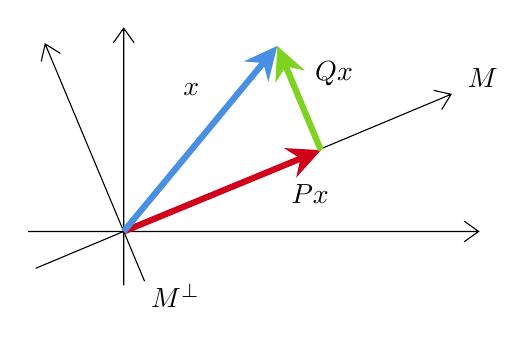
\begin{tikzpicture}[x = 0.75pt, y = 0.75pt, yscale = - 1, xscale = 1]
%uncomment if require: \path (0, 184); %set diagram left start at 0, and has height of 184

%Shape: Axis 2D [id: dp7134109691601231]
\draw (198, 127.91) - - (415, 127.91)(244, 30) - - (244, 153.91) (408, 122.91) - - (415, 127.91) - - (408, 132.91) (239, 37) - - (244, 30) - - (249, 37);
%Shape: Axis 2D [id: dp2976528104012621]
\draw (201.57, 145.68) - - (401.72, 61.83)(206.17, 37.6) - - (254.05, 151.89) (393.33, 59.93) - - (401.72, 61.83) - - (397.2, 69.15) (204.26, 45.99) - - (206.17, 37.6) - - (213.49, 42.13);
%Straight Lines [id: da6603280695196603]
\draw [color = {rgb, 255: red, 208; green, 2; blue, 27}, draw opacity = 1][line width = 2.25] (244, 127.91) - - (334.38, 90.66);
\draw [shift = {(339, 88.75)}, rotate = 517.6] [fill = {rgb, 255: red, 208; green, 2; blue, 27}, fill opacity = 1][line width = 0.08] [draw opacity = 0] (16.07, - 7.72) - - (0, 0) - - (16.07, 7.72) - - (10.67, 0) - - cycle;
%Straight Lines [id: da12421560052711267]
\draw [color = {rgb, 255: red, 74; green, 144; blue, 226}, draw opacity = 1][line width = 2.25] (244, 127.91) - - (314.81, 42.38);
\draw [shift = {(318, 38.53)}, rotate = 489.62] [fill = {rgb, 255: red, 74; green, 144; blue, 226}, fill opacity = 1][line width = 0.08] [draw opacity = 0] (16.07, - 7.72) - - (0, 0) - - (16.07, 7.72) - - (10.67, 0) - - cycle;
%Straight Lines [id: da9584665613249306]
\draw [color = {rgb, 255: red, 126; green, 211; blue, 33}, draw opacity = 1][line width = 2.25] (339, 88.75) - - (319.93, 43.15);
\draw [shift = {(318, 38.53)}, rotate = 427.31] [fill = {rgb, 255: red, 126; green, 211; blue, 33}, fill opacity = 1][line width = 0.08] [draw opacity = 0] (16.07, - 7.72) - - (0, 0) - - (16.07, 7.72) - - (10.67, 0) - - cycle;

% Text Node
\draw (408.5, 48.4) node [anchor = north west][inner sep = 0.75pt] {$M$};
% Text Node
\draw (256, 151.9) node [anchor = north west][inner sep = 0.75pt] {$M^{\perp}$};
% Text Node
\draw (271.5, 55.4) node [anchor = north west][inner sep = 0.75pt] {$x$};
% Text Node
\draw (335, 44.9) node [anchor = north west][inner sep = 0.75pt] {$Qx$};
% Text Node
\draw (323.5, 103.9) node [anchor = north west][inner sep = 0.75pt] {$Px$};
\end{tikzpicture}
\end{figure}
\FloatBarrier

\newpage


\section{Basi hilbertiane e serie di Fourier generalizzata}

\begin{defn}
Sia $H$ uno spazio di Hilbert, $\dim H=+\infty$. Sia $\{e_n\}_{n=1,2,\dots}\subset H$ una successione di vettori di $H$. Si dice che $\{e_n\}$ genera $H$ se $\forall x\in H$ e $\forall\Ec>0$ esiste una successione $\{\lambda_n\}_{n=1,\dots,N}$ tale che
$$
\left\|x-\sum_{n=1}^N\lambda_ne_n \right\|<\Ec
$$
\end{defn}
Ciò significa che è possibile generare uno spazio di dimensione \underline{infinita} con una combinazione lineare \underline{finita} di $\{e_n\}$, attraverso una \textit{tanto buona quanto si vuole} approssimazione.

\begin{rem}
Definendo le somme parziali della serie con $S_N=\sum_{n=1}^N\lambda_ne_n$ si può tradurre la relazione soprastante in 
$$
\lim_{N\to+\infty}S_N=x
$$
dove però è andato perduto il senso di convergenza in norma.
\end{rem}

\begin{defn}
[Base hilbertiana]
Sia $H$ uno spazio di Hilbert, $\dim H=+\infty$. Una successione di vettori $\{e_n\}_{n=1,2,\dots}\subset H$ si dice base hilbertiana, o sistema ortonormale completo, se $\{e_n\}$ genera $H$ ed è ortonormale, ovvero
$$
(e_n,e_m)=\delta_{nm}=
\begin{cases}
0 &m\neq n \\ 1 &m=n
\end{cases} \qquad \qquad \Vert e_n \Vert =1\ \ \forall n
$$
\end{defn}

Osserviamo due cose:
\begin{enumerate}
    \item Non essendo finita, una base hilbertiana non è una base nel senso dell'algebra lineare, ma è la cosa che più le si avvicina in dimensione infinita.
    \item La condizione $\Vert e_n \Vert =1$ è già implicita in $(e_n,e_m)=\delta_{nm}$.
\end{enumerate}

Se avessimo un generico spazio vettoriale $X$ finito potremmo scrivere
$$
x=\sum_{n=1}^Nc_ne_n
$$
e se la base fosse ortonormale potremmo addirittura calcolare i coefficienti della combinazione lineare tramite il prodotto scalare
$$
(x,e_n)=\left(\sum_{n=1}^Nc_ne_n,e_n\right)=\sum_{n=1}^Nc_n(e_n,e_n)=c_n
$$
Con una base hilbertiana vale un qualcosa di \textit{mooolto} simile:
\begin{thm}
\label{teoHNOsepa}
Sia $H$ uno spazio di Hilbert, $\dim H=+\infty$. Sia $\{e_n\}_{n=1,2,\dots}\subset H$ una base hilbertiana. Allora un qualsiasi $x\in H$ si scrive come \textbf{serie di Fourier generalizzata}
\begin{equation*}
\boxed{x = \sum^{+\infty}_{n = 1}(x, e_{n}) e_{n}}
\end{equation*}
I coefficienti $(x,e_n)=:\lambda_n$ della combinazione sono detti \textbf{coefficienti di Fourier} di $x$ rispetto $\{e_n\}$, e, come nel caso finito, sono dati da un prodotto scalare.
\end{thm}

Riprendendo il discorso di inizio pagina, abbiamo che la serie di Fourier generalizzata converge se e solo se
$$
\forall\Ec>0 \quad \exists N\in \NN \quad \text{t.c.}\quad \left\|x-\sum_{n=1}^N(x,e_n)e_n\right\|\leq \Ec
$$

\newpage

\section{Serie di Fourier elementare}

In questo paragrafo si parlerà di funzioni misurabili secondo Lebesgue, cosa che verrà ampiamente approfondita nel prossimo capitolo.

\begin{defn}
Lo spazio delle funzioni a quadrato integrabile è
$$L^2\left([a,b]\right):=\left\{f:[a,b]\to\RR\text{ Lebesgue misurabili t.c. }\displaystyle\int_a^bf^2(x)\dx<+\infty \right\}$$
ed è uno spazio vettoriale.
\end{defn}
Su $L^2$ introduciamo la funzione prodotto scalare
\begin{equation*}
(f,g)=\int_a^bf(x)g(x)\dx
\end{equation*}
e la funzione norma
\begin{equation*}
\Vert f \Vert ^2=\int_a^bf^2(x)\dx=(f,f)
\end{equation*}
in modo tale che $L^2$ sia uno spazio di Hilbert.

Consideriamo ora come spazio di lavoro $L^{2}([ - \pi, \pi])$ e la base
\begin{equation*}
\Bc = \left\{\frac{1}{\sqrt{2\pi}}, \frac{\cos x}{\sqrt{\pi}}, \frac{\sin x}{\sqrt{\pi}}, \frac{\cos2x}{\sqrt{\pi}}, \frac{\sin2x}{\sqrt{\pi}}, \dotsc, \frac{\cos kx}{\sqrt{\pi}}, \frac{\sin kx}{\sqrt{\pi}}, \dotsc  \right\}
\end{equation*}

Si può dimostrare che $\Bc$ è una base hilbertiana secondo il prodotto scalare definito qui sopra.

Allora vale il teorema della serie di Fourier generalizzata, cioè
possiamo costruire ogni funzione $f$ dello spazio di Hilbert $L^2\left([-\pi,\pi]\right)$ tramite la base $\Bc$ come 
\begin{equation*}
\boxed{f(x)=\frac{a_0}{\sqrt{2\pi}}+\sum_{k=1}^{+\infty}\left(a_k\,\frac{\cos kx}{\sqrt{\pi}}+b_k\,\frac{\sin kx}{\sqrt{\pi}}\right)}
\end{equation*}
Questa è la cosiddetta \textbf{serie di Fourier} (elementare) di coefficienti
\begin{equation*}
a_{k} =\left(f,\frac{\cos kx}{\sqrt{\pi}}\right) = \frac{1}{\sqrt{\pi}}\int^{\pi}_{- \pi} f(x)\cos(kx) \dx\qquad
b_{k} = \left(f,\frac{\sin kx}{\sqrt{\pi}}\right) = \frac{1}{\sqrt{\pi}}\int^{\pi}_{- \pi} f(x)\sin(kx) \dx
\end{equation*}

Come per la serie di Fourier generalizzata, anche quella elementare converge se e solo se
$$
\forall\Ec>0 \quad \exists N\in \NN \quad \text{t.c.}\quad \left\|f(x)-\left[\frac{a_0}{\sqrt{2\pi}}+\sum_{k=1}^{+\infty}\left(a_k\,\frac{\cos kx}{\sqrt{\pi}}+b_k\,\frac{\sin kx}{\sqrt{\pi}}\right)\right]\right\|\leq \Ec
$$

Per concludere, è bene notare che con una piccola modifica alla base
\begin{equation*}
\Bc = \left\{\frac{1}{\sqrt{2}}, \cos x, \sin x, \cos 2x, \sin 2x, \dotsc,\cos kx,\sin kx,\dotsc \right\}
\end{equation*}
e al prodotto scalare
\begin{equation*}
(f,g):=\frac{1}{\pi}\int_{-\pi}^\pi f(x)g(x)\dx \qquad \Vert f\Vert^2=\frac{1}{\pi}\int_{-\pi}^\pi f^2(x)\dx
\end{equation*}
si ottiene
\begin{gather*}
\boxed{f(x)=\frac{a_0}{2}+\sum_{k=1}^{+\infty}\left(a_k\cos kx+b_k\sin kx\right)} \\
a_{k} = (f, \cos kx) = \frac{1}{\pi}\int^{\pi}_{- \pi} f(x)\cos(kx) \dx\qquad
b_{k} = (f, \sin kx) = \frac{1}{\pi}\int^{\pi}_{- \pi} f(x)\sin(kx) \dx
\end{gather*}

\newpage

\section{Spazi separabili}

In questa sezione cercheremo di capire se, dato uno spazio di Hilbert generico, esiste una base hilbertiana. Per fare ciò riprendiamo le nozioni di numerabilità e di densità:

\begin{defn}[Insieme numerabile]
Si dice che l'insieme $A$ è numerabile se può essere messo in corrispondenza biunivoca con $\NN$.
\end{defn}
In pratica significa che possiamo \textit{mettere in fila} i suoi elementi:$A=\{a_1,a_2,a_3,\dots\}$.
\begin{defn}[Spazio denso]
Sia $X$ uno spazio normato e siano $A\subseteq B\subseteq X$. Si dice che $A$ è denso in $B$ se $\overline{A}=B$.
\end{defn}
In pratica significa che possiamo sempre costruire una successione in $V$ che approssima, nel senso della norma, lo spazio $H$.
\begin{exa}
$\RR$ non è numerabile. $\QQ$ è denso in $\RR$.
\end{exa}

Siamo pronti:

\begin{defn}[Spazio separabile]
Uno spazio $H$ di Hilbert si dice separabile se ammette un sottoinsieme denso e numerabile, ovvero se $\exists\,V\subset H$ numerabile tale che $\overline{V}=H$.
\end{defn}

\begin{thm}
Uno spazio $H$ di Hilbert, $\dim H=+\infty$, ammette una base hilbertiana se e solo se $H$ è separabile.
\end{thm}

\begin{proof}\leavevmode
\begin{enumerate}
    \item [($\Rightarrow$)] Sia $\{e_n\}$ la base hilbertiana di $H$. Allora la somma parziale $S_N$ è numerabile e approssima nel senso della norma $x\in H$, per cui $H$ è separabile.
    \item [($\Leftarrow$)] Sia $V\subset H$ denso e numerabile. Allora è possibile costruire una base hilbertiana di $H$ usando l'\textbf{algoritmo di ortogonalizzazione di Gram-Schmidt}:
    \begin{align*}
    V&=\left\{x_1,x_2,x_3,\dots \right\} \\
    e_1&=\frac{x_1}{\Vert x_1 \Vert} \\
    e_2&=\frac{x_2-(x_2,e_1)e_1}{\Vert x_2-(x_2,e_1)e_1 \Vert} \\
    e_3&=\frac{x_3-(x_3,e_1)e_1-(x_3,e_2)e_2}{\Vert x_3-(x_3,e_1)e_1-(x_3,e_2)e_2 \Vert} \\
    &\ \vdots
    \end{align*}
    Infatti i vettori $e_n$ sono ortogonali tra loro e hanno norma unitaria per costruzione; inoltre, essendo $V$ denso, generano $H$.
\end{enumerate}
\end{proof}

\newpage

\section{Serie di Fourier generalizzate su spazi separabili}

Ora riprendiamo a parlare di serie di Fourier generalizzate.

Grazie alla nozione di spazio di Hilbert separabile possiamo re-interpretare il teorema (\ref{teoHNOsepa}): è possibile sostituire all'ipotesi di esistenza della base hilbertiana $\{e_n\}$ la separabilità dello spazio di Hilbert considerato.

In ogni caso, una volta che sappiamo che esiste $\{e_n\}$ (che sia diretta conseguenza della separabilità oppure un'ipotesi) ha senso la seguente
$$
\Vert x\Vert^2=\sum_{n=1}^{+\infty} (x,e_n)^2 \qquad\qquad  \textbf{identità di Parseval}
$$
dove si ricorda che $(x,e_n):=\lambda_n$ sono i coefficienti di Fourier di $x$ rispetto la base $\{e_n\}$. Tale identità è banalmente verificabile:
\begin{align*}
\Vert x \Vert^2&=(x,x)=\left(\sum_{n=1}^{+\infty}(x,e_n)e_n,\sum_{k=1}^{+\infty}(x,e_k)e_k\right)=\\
&=\sum_{n=1}^{+\infty}\sum_{k=1}^{+\infty} (x,e_n)(x,e_k)\underbrace{(e_n,e_k)}_{\delta_{nk}}=\sum_{n=1}^{+\infty} (x,e_n)^2
\end{align*}

L'identità di Parseval permette di dire che la successione $\{\lambda_n\}$ dei coefficienti di Fourier è una successione a quadrato sommabile, ovvero $\{\lambda_n\}\subset \ell^2$ (se si parla di serie di Fourier elementare si ha $\{a_n\},\ \{b_n\}\in\ell^2$).

In realtà Parseval suggerisce qualcosa in più: è possibile definire un'applicazione $L:H\to\ell^2$ che associa ad ogni $x\in H$ la successione $\lambda=\{\lambda_n\}=\{(x,e_n)\}\subset\ell^2$ dei suoi coefficienti di Fourier rispetto alla base $\{e_n\}$; tale applicazione è ovviamente \underline{lineare}
$$
(ax+by,e_n)=a(x,e_n)+b(y,e_n)
$$
\underline{isometrica} (stessa metrica su dominio e codominio)
$$
\Vert Lx \Vert_{\ell^2}=\Vert \lambda \Vert_{\ell^2}=\left(\sum_{n=1}^{+\infty}\lambda_n^2\right)^{1/2} =\Vert x \Vert_H
$$
e di conseguenza anche \underline{iniettiva} e \underline{continua}. 

Tutto questo, in \textit{matematichese}, si traduce in
\begin{thm}
Sia $H$ uno spazio di Hilbert separabile di dimensione infinita. Allora $H$ è isomorfo e isometrico allo spazio $\ell^2$, cioè esiste un \textbf{isomorfismo isometrico}
\begin{align*}
L:H&\to\ell^2 \\
x&\mapsto Lx=\{(x,e_n)\}
\end{align*}
\end{thm} 

\begin{proof}
Per dimostrare l'asserto dobbiamo dimostrare che $H$ e $\ell^2$ sono isometrici, cioè sono dotati della stessa metrica, e isomorfi, cioè $L$ è una mappa lineare continua e biunivoca.

Ma che i due spazi sono isometrici
\begin{equation*}
\Vert Lx \Vert_{\ell^2}=\Vert x \Vert_H \qquad \forall x\in H
\end{equation*}
e che $L$ è lineare continua e iniettiva l'avevamo già dedotto dall'identità di Parseval.

Dunque l'unica cosa che veramente viene aggiunta da questo teorema è la \underline{suriettività} di $L$: per dimostrare quest'ultima bisogna prendere $a=(a_1,a_2,\dots)\in\ell^2$ e verificare che $Lx=a$. 

Consideriamo allora la somma parziale
$$
x_n:=\sum_{k=1}^na_ke_k
$$
Sappiamo due cose: che $\sum_{k=1}^\infty a_k^2$ converge (per definizione di $\ell^2$) e che gli $e_k$ sono ortonormali (per definizione di base hilbertiana). Da ciò si deduce che per ogni $\Ec>0$ esiste $N\in \NN$ tale che per ogni $n>m>N$
$$
\Vert x_n-x_m\Vert_H^2=\left\|\sum_{k=m+1}^n a_ke_k\right\|^2=\sum_{k=m+1}^n a_k^2<\Ec
$$
Pertanto la successione $\{x_n\}$ è di Cauchy in $H$ ed essendo quest'ultimo completo esiste $x\in H$ tale che $x_n\to x$. Si verifica immediatamente che i coefficienti di Fourier di $x$ coincidono con gli $a_k$ e quindi $Lx=a$: $L$ è suriettiva.
\end{proof}

\begin{rem}
Tale teorema è l'estensione infinito-dimensionale al teorema che mette in corrispondenza un insieme qualsiasi di dimensione $n$ a $\RR^n$.
\end{rem}


\section{Convergenza, continuità e derivabilità della serie di Fourier elementare}

Studiamo in maniera più approfondita lo spazio di Hilbert separabile $L^2([-\pi,\pi])$ con il prodotto scalare definito da
\begin{equation*}
(f,g)_{L^2}:=\frac{1}{\pi} \int_{-\pi}^\pi fg\qquad \forall f,g\in L^2([-\pi,\pi])
\end{equation*}
e con la norma indotta
\begin{equation*}
\Vert f\Vert_{L^2}^2=\frac{1}{\pi} \int_{-\pi}^\pi f^2\qquad \forall f\in L^2([-\pi,\pi])
\end{equation*}
Consideriamo poi l'insieme (numerabile) di funzioni
\begin{equation*}
\Bc = \left\{\frac{1}{\sqrt{2}}, \cos x, \sin x, \cos 2x, \sin 2x, \dotsc,\cos kx,\sin kx,\dotsc \right\}
\end{equation*}
Si può dimostrare che tale base è hilbertiana in $L^2([-\pi,\pi])$ rispetto al prodotto scalare sopra definito, perciò data una qualunque funzione $f\in L^2([-\pi,\pi])$ è sempre possibile determinare due successioni reali $\{a_n\}$ e $\{b_n\}$ tali che
\begin{equation*}
\boxed{f(x)=\frac{a_0}{2}+\sum_{k=1}^{+\infty}\left(a_k\cos kx+b_k\sin kx\right)}
\end{equation*}
dove
\begin{align*}
a_{k} &= (f, \cos kx) = \frac{1}{\pi}\int^{\pi}_{- \pi} f(x)\cos(kx) \dx\\
b_{k} &= (f, \sin kx) = \frac{1}{\pi}\int^{\pi}_{- \pi} f(x)\sin(kx) \dx
\end{align*}
Analogamente a quanto avevamo già detto, la serie di Fourier elementare converge in $L^2$ se e solo se 
$$
\forall\Ec>0 \quad \exists N\in \NN \quad \text{t.c.}\quad \left\|f(x)-\left[\frac{a_0}{2}+\sum_{k=1}^{+\infty}\left(a_k\cos kx+b_k\sin kx\right)\right]\right\|\leq \Ec
$$
il che equivale a dire che $\{S_N\}$ \textbf{converge in media quadratica} a $f$
\begin{equation*}
\lim\limits_{N\rightarrow + \infty}\left[\int^{\pi}_{- \pi}\left[f(x) - S_{N}(x)\right]^{2} \dx\right] = 0 \qquad \text{con}\qquad S_{N}(x) = \frac{a_{0}}{2} + \sum\limits^{N}_{n = 1}\left(a_n\cos nx+b_n\sin nx\right)
\end{equation*}
Inoltre, l'identità di Parseval diventa 
$$
\Vert f \Vert_{L^2}^2=\pi\left\{\frac{a_0^2}{2}+\sum_{k=1}^{+\infty}\left(a_k^2+b_k^2\right)\right\}
$$
che sembra un po' l'estensione infinito-dimensionale del teorema di Pitagora.

\begin{rem}
Quanto sopra descritto è possibile solamente nel caso in cui la funzione $f\in L^2$ sia periodica di periodo $2\pi$, anche si può chiaramente generalizzare il risultato a periodi generici $T$
\begin{equation*}
f(x) = \frac{a_{0}}{2} + \sum\limits^{\infty}_{n = 1}\left[a_{n}\cos\left(\frac{2n\pi}{T} x\right) + b_{n}\sin\left(\frac{2n\pi}{T} x\right)\right] \qquad \forall f\in L^{2}\left(\left[ - \frac{T}{2}, \frac{T}{2}\right]\right)
\end{equation*}
con prodotto scalare
\begin{equation*}
(f, g) = \frac{2}{T}\int^{T/2}_{- T/2} f(x) g(x) \dx
\end{equation*}
e quindi
\begin{align*}
a_{n} &= \frac{2}{T}\int^{T/2}_{- T/2} f(x)\cos\left(\frac{2n\pi}{T} x\right) \dx \\
b_{n} &= \frac{2}{T}\int^{T/2}_{- T/2} f(x)\sin\left(\frac{2n\pi}{T} x\right) \dx
\end{align*}
Osserviamo però che il calcolo dei coefficenti $a_,b_n$ è possibile nella sola ipotesi in cui $f$ sia solamente integrabile, ovvero $f\in L^1$; tuttavia in questo spazio vengono a mancare sia l'identità di Parseval che particolari proprietà di convergenza (calma, ora le vediamo), che sono invece presenti nello spazio più piccolo $L^2$.
\end{rem}

\subsection{Sulla continuità}

Vediamo ora altri tipi di convergenza delle serie di Fourier.

\begin{thm}[Criterio di Dirichlet]
Se $a_n,b_n\downarrow0$, cioè le successioni decrescono monotamente a 0 e sono positive, allora la serie di Fourier $f(x)$ converge puntualmente in $[-\pi,\pi]$.
\end{thm}

\begin{thm}[Criterio di Weierstrass]
Se $\displaystyle\sum_{k=1}^{+\infty}\left(|a_k|+|b_k|\right)<+\infty$ allora la serie di Fourier $f(x)$ converge uniformemente in $[-\pi,\pi]$.
\end{thm}
\begin{proof}
Posto 
$$
c_k=\sup_{x\in[-\pi,\pi]} |a_k\cos kx+b_k\sin kx|
$$
si ha
$$
\sum_{k=1}^{+\infty} c_k \leq \sum_{k=1}^{+\infty} |a_k+b_k| \leq \sum_{k=1}^{+\infty}\left(|a_k|+|b_k|\right)<+\infty 
$$
e quindi la serie di Fourier converge uniformemente.
\end{proof}

\begin{thm}[Continuità]
Se la serie di Fourier $f(x)$ converge uniformemente in $[-\pi,\pi]$ allora $f\in\Cc^0\left([-\pi,\pi]\right)$ e in particolare $f(-\pi)=f(\pi)$; inoltre, per la periodicità della funzione, si ha continuità in tutto $\RR$.
\end{thm}

Vi sono tuttavia diversi risultati che garantiscono direttamente la convergenza puntuale senza coinvolgere la convergenza uniforme o il criterio di Dirichlet. Vediamone uno in particolare.

\begin{defn}[Funzione regolare a tratti]
Una funzione $f: [-\pi, \pi]\rightarrow \RR$ si dice regolare a tratti se $f$ è limitata in $[-\pi, \pi]$ e l'intervallo si può scomporre in un numero finito di sottointervalli su ciascuno dei quali $f$ è continua e derivabile; inoltre agli estremi di ogni sottointervallo, esistono finiti i limiti sia di $f$ che di $f'$.
\end{defn}

Tale classe di funzioni è molto ampia, perché ci possono essere dei punti angolosi e persino delle discontinuità di tipo salto; sono però escluse funzioni con asintoti verticali o punti a tangenza verticale.

\begin{thm}
[Convergenza puntuale per funzioni regolari a tratti]
Sia $f: [ - \pi, \pi]\rightarrow \RR$ regolare a tratti. Allora la serie di Fourier associata a $f$ converge in ogni punto $x_0\in [ - \pi, \pi]$ alla media dei limiti destro e sinistro:
$$
f(x_0)=\frac{a_0}{2}+\sum_{n=1}^{+\infty}\left(a_n\cos nx_0+b_n\sin nx_0\right)=\frac{f(x_0^+)+f(x_0^-)}{2}
$$
In particolare, se $f$ è continua in $x_0$, allora la serie di Fourier converge a $f(x_0)$.
\end{thm}

\subsection{Sulla derivazione}

Osserviamo che derivando la serie di Fourier si ottiene
\begin{equation*}
f'(x) = \sum\limits^{\infty}_{n = 1}a_nn(-\sin nx)+b_nn\cos nx
\end{equation*}
che converge uniformemente, e quindi $f\in\Cc^1(\RR)$, se
\begin{equation*}
\sum\limits^{\infty}_{n = 1} n(| a_{n}| + | b_{n}|) < \infty
\end{equation*} 
Iterando il ragionamento otteniamo il seguente
\begin{thm}[Derivabilità]
$f\in\Cc^k(\RR)$ se
\begin{equation*}
\sum\limits^{\infty}_{n = 1} n^{k}(| a_{n}| + | b_{n}|) < \infty
\end{equation*}
\end{thm}

Ad ogni derivazione la serie diventa ``meno infinitesima'' a causa della moltiplicazione per $n$; questo significa che ad una maggiore velocità di decadimento dei coefficienti corrisponde una maggiore regolarità della serie.

\begin{exa}
La serie trigonometrica
$$
\sum_{n=1}^{+\infty}\left(\frac{\cos nx}{n^2}+\frac{\sin nx}{n^2}\right)
$$
converge uniformemente. Derivando tale serie otteniamo
$$
\sum_{n=1}^{+\infty}\left(\frac{\cos nx}{n}-\frac{\sin nx}{n}\right)
$$
e ci accorgiamo che la situazione è ``peggiorata''.
\end{exa}
Possiamo concludere che, a differenza delle serie di potenze, le serie di Fourier possono perdere la convergenza dopo una derivazione; questo però non è del tutto a loro sfavore: infatti non ha senso usare una serie di potenze per approssimare una funzione che non è $\Cc^{\infty}$, ma ha perfettamente senso farlo con una serie di Fourier.

Concludiamo con 
\begin{thm}
Se i coefficienti della serie di Fourier decrescono esponenzialmente, ovvero 
$$
|a_k|+|b_k|\leq c_1e^{-c_2k} \qquad \qquad c_1,c_2>0
$$
allora $f\in\Cc^\infty$.
\end{thm}

\subsection{Forma esponenziale delle serie di Fourier}

La ben nota formula di Eulero per l'esponenziale di un immaginario puro, $e^{i\theta}=\cos\theta+i\sin\theta$, suggerisce di scrivere una serie di Fourier utilizzando gli esponenziali.

Ricaviamo
\begin{equation*}
\cos(nx) = \frac{e^{inx} + e^{- inx}}{2}\qquad \qquad \sin(nx) = \frac{e^{inx} - e^{- inx}}{2i}
\end{equation*}
e dunque ponendo
\begin{equation*}
c_n=\frac{a_n-ib_n}{2}\qquad \qquad c_{-n}=\frac{a_n+ib_n}{2}=\overline{c_n}
\end{equation*}
si ottiene la \textbf{forma esponenziale} della serie di Fourier
\begin{equation*}
\boxed{f(x) = \sum\limits_{n\in\ZZ} c_{n} e^{inx}}
\end{equation*}
dove l'uguaglianza è da intendersi come convergenza in $L^2$ delle somme parziali rispetto alla norma indotta dal prodotto scalare
$$
(f, g) = \frac{1}{2\pi}\int^{\pi}_{- \pi} f(x)\,\overline{g(x)} \dx
$$
Come per la serie di seni e coseni, i coefficienti di Fourier si calcolano con il prodotto scalare
\begin{align*}
c_{n} &=\frac{a_n-ib_n}{2}=\frac{1}{2\pi}\int^{\pi}_{- \pi} f(x)\, e^{- inx} \dx \\
c_{-n} &=\frac{a_n+ib_n}{2} =\frac{1}{2\pi}\int^{\pi}_{- \pi} f(x)\, e^{ inx} \dx
\end{align*}
dove si è presa la base ortonormale (si può dimostrare che è anche hilbertiana)
$$
\left\{\frac{e^{inx}}{\sqrt{2\pi}}  \right\}_{n\in\ZZ}
$$
Inoltre, si ha $a_n=c_n+c_{-n}$ e $b_n=i(c_n-c_{-n})$ e l'identità di Parseval assomiglia sempre di più al teorema di Pitagora:
$$
\frac{1}{2\pi}\int^{\pi}_{- \pi} f^2(x) \dx =\sum_{n\in\ZZ} c_n^2
$$
\begin{rem}
Esistono tante altre basi ortonormali (hilbertiane) che permettono di riscrivere a piacere la serie di Fourier elementare: la base di Legendre, Chebychev, Bessel, ecc. Ecco che capiamo perché si è voluto generalizzare il concetto di serie di Fourier elementare con il concetto di serie di Fourier generalizzata!
\end{rem}


\chapter{Integrale di Lebesgue e spazi \texorpdfstring{$L^p$}{C}}

La teoria dell'integrazione di Lebesgue è un importante strumento nelle applicazioni ed è quindi necessario averne una buona conoscenza. In questo capitolo richiameremo le definizioni di base e i principali risultati.\\
Se confrontata con la più intuitiva teoria dell'integrazione secondo Riemann, la teoria dell'integrazione secondo Lebesgue introduce una più ampia classe di funzioni integrabili; tale ampliamento del concetto di integrabilità fa sì che lo spazio $L^1$ delle funzioni integrabili secondo Lebesgue acquisisca la struttura di spazio di Banach, che può essere estesa in genere a tutti gli spazi $L^p$.

\section{Integrale di Riemann (accenni)}

Ricordiamo dal corso di AN1 che, dette 
\begin{align*}
S(\Pc)&=\text{somma superiore}\\
s(\Pc)&=\text{somma inferiore}
\end{align*}
e
\begin{align*}
S&=\inf_{\Pc}S(\Pc) \\
s&=\sup_{\Pc}s(\Pc)
\end{align*}
la funzione $f:[a,b]\to\RR$ è Riemann-integrabile se e solo se $s=S$, e in particolare l'integrale definito di Riemann di $f$ in $x$ è
\begin{equation*}
s=S=:\int_{a}^{b}f(x)\dx
\end{equation*}
Come possiamo vedere, la definizione di integrale di Riemann è molto semplice e intuitiva. In pratica, si tratta di approssimare una funzione limitata con due funzioni ``a gradini'' che forniscono due approssimazioni, una per eccesso e una per difetto; se riusciamo ad avere due stime che differiscono per quantità arbitrariamente piccole diremo che la funzione è integrabile secondo Riemann.

A causa della sua semplicità, il rischio che si corre è quello di non riuscire a integrare funzioni ``strane''. Si consideri per esempio la funzione di Dirichlet $f$ definita nell'intervallo $[0,1]$ da
\begin{equation*}
f(x):=\begin{cases}
1 &x\in[0,1]\cap\QQ \\
0 &x\in[0,1]\setminus\QQ
\end{cases}
\end{equation*}
Per qualunque suddivisione di $[0,1]$ risulta $S=1$ e $s=0$ quindi $f$ non è integrabile secondo Riemann.

Non ci occupiamo qui di elencare le proprietà dell'integrale di Riemann, e passiamo direttamente a definire l'integrale di Lebesgue.

\section{Integrale di Lebesgue}

\subsection{Misura di Lebesgue}
Chiamiamo \textbf{plurirettangolo} (o plurintervallo) l'unione $P$ di un numero finito di intervalli $[a_i,b_i]$
\begin{equation*}
P\subset \RR^{n}, \ \ P = [a_{1}, b_{1}] \times \dotsc \times [a_{n}, b_{n}]
\end{equation*}
La \textbf{misura} del plurirettangolo viene definita come
\begin{equation*}
|P| = (b_{1} - a_{1}) \dotsc (b_{n} - a_{n})
\end{equation*}

\begin{defn}
Sia $A$ un aperto limitato non vuoto di $\RR^n$; la misura di $A$ è l'estremo superiore delle misure dei plurirettangoli contenuti in $A$:
\begin{equation*}
|A| := \sup \left\{|P|, P\in \text{plurirettangoli}, P\subset A\right\}
\end{equation*}
\end{defn}

\begin{defn}
Sia $C$ un chiuso limitato non vuoto di $\RR^n$; la misura di $C$ è l'estremo inferiore delle misure dei plurirettangoli contenuti in $C$:
\begin{equation*}
| C| := \inf\left\{| P|, P\in \text{plurirettangoli}, P\supset C\right\}
\end{equation*}
\end{defn}

Possiamo ora considerare un generico insieme di $\RR^n$:
\begin{defn}
Sia $E$ un insieme limitato di $\RR^n$. Si definiscono
\begin{itemize}
\item \textbf{misura esterna} di $E$, $| E|^{*} := \inf\left\{| A|, A\ \text{aperto}, A\supseteq E\right\}$
\item \textbf{misura interna} di $E$, $| E|_{*} := \sup \left\{| C|, C\ \text{chiuso}, C\subseteq E\right\}$
\end{itemize}
\end{defn}

\begin{rem}
Se $E$ è aperto o chiuso si ha ovviamente $| E|^{*}=|E|=| E|_{*}$. Inoltre per ogni insieme $E$ limitato risulta $| E|^{*}\geq | E|_{*}$.
\end{rem}

\begin{defn}
\label{Leb_limitato}
Un insieme $E$ si dice misurabile secondo Lebesgue se $| E|^{*} = | E|_{*}$.
\end{defn}
Questo concetto di misurabilità è stato introdotto soltanto per insiemi limitati; tuttavia, nelle applicazioni può essere utile estendere la nozione di misurabilità a insiemi illimitati. A tale scopo, dopo aver osservato che l'intersezione di due insiemi (limitati) misurabili è misurabile, diamo la seguente
\begin{defn}
\label{Leb_illimitato}
Un insieme $E\subseteq\RR^n$ (anche illimitato) è \textbf{misurabile secondo Lebesgue} se per ogni $r>0$ l'insieme $E\cap B_{r}$ è misurabile secondo la definizione (\ref{Leb_limitato}), con $B_r:=\{x\in\RR^n\ :\ |x|<r \}$. In tal caso si definisce
$$
| E| : = \lim\limits_{r\rightarrow + \infty}| E\cap B_{r}| \in[0,+\infty]
$$
\end{defn}
\begin{rem}
Scegliendo $r>0$ abbastanza grande (in modo che $E\cap B_{r}=E$) si deduce che gli insiemi misurabili secondo la definzione (\ref{Leb_limitato}) sono misurabili anche secondo la definizone (\ref{Leb_illimitato}). Abbiamo quindi esteso corretamente il concetto di misurabilità secondo Lebesgue.
\end{rem}
Da ora in poi con misurabilità secondo Lebesgue si intenderà la nozione intodotta dalla definizone (\ref{Leb_illimitato}).

\newpage

\begin{thm}
Sia $\{E_i\}$ una successione di insiemi misurabili di $\RR^n$. Allora l'insieme 
$$
E:=\bigcup_{i=1}^\infty E_i
$$ 
è misurabile e vale la seguente disuguaglianza (subadditività numerabile della misura)
$$
|E|\leq \sum_{i=1}^\infty |E_i|
$$
In particolare, se $E_i\cap E_j=\varnothing$ per ogni $i\neq j$ allora vale l'uguale nella formula (additività numerabile della misura). Inoltre, se supponiamo che la successione $\{E_i\}$ sia non decrescente rispetto all'inclusione, cioè $E_1\subseteq E_2\subseteq\dots$, allora
$$
|E|=\lim_{i\to\infty}|E_i|
$$ 
\end{thm}
\begin{rem}
Usando tale teorema si può dimostare un asserto analogo anche per $\displaystyle\bigcap_{i=1}^\infty E_i$.
\end{rem}
Per comprendere l'importanza di tale teorema si osservi che un insieme formato da un'infinità numerabile di punti ha misura nulla!

All'atto pratico, quasi tutti gli insiemi sono misurabili; quelli non misurabili sono casi piuttosto ``patologici'' (un celebre esempio è quello dovuto a \textit{Vitali}).

\subsection{Funzioni misurabili}

\begin{defn}
Una funzione $f: A\subset \RR^{n}\rightarrow \RR$ è \textbf{misurabile} se per ogni $c\in\RR$ l'insieme
\begin{equation*}
\{x\in A\ :\ f(x) < c\}
\end{equation*}
è misurabile secondo Lebesgue.
\end{defn}

\begin{defn}
Sia $A\subseteq\RR^n$ misurabile e siano $f,g:A\to\RR$ misurabili. Si dice che $f$ è uguale a $g$ \textbf{quasi ovunque} in $A$ se
$$
|\{x\in A\ :\ f(x)\neq g(x)\}|=0
$$
Si dice inoltre che una certa proprietà vale quasi ovunque in $x$ se l'insieme degli $x\in A$ per i quali tale proprietà non vale è un insieme di misura nulla.
\end{defn}

Accenniamo solamente al fatto che da qui possiamo andare a definire le somme inferiori $s$ e superiori $S$ ``alla Lebesgue'' di $f$. Ma quello che ci interessa davvero è il concetto di integrale.

\newpage

\subsection{Integrale di Lebesgue}

Procediamo per passi successivi:
\begin{enumerate}
    \item [(i)] Funzioni misurabili e limitate su insiemi di misura finita.

    \begin{defn}
    Sia $A\subset\RR^n$ di misura finita e $f:A\to\RR$ misurabile e limitata. Allora
    $$
    \sup s = \inf S =:\int_A f(x) \dx
    $$
    viene detto integrale di Lebesgue di $f$ su $A$.
    \end{defn}

    \item [(ii)] Funzioni misurabili nonnegative (non necessariamente limitate) su insiemi di misura finita.

    Sia $A\subseteq\RR^n$ di misura finita e $f:A\to\RR$ misurabile e nonnegativa. Per ogni $\lambda>0$ definiamo
    $$
    f_\lambda(x):=\begin{cases}
    f(x) &f(x)\leq\lambda \\
    \lambda &f(x)>\lambda
    \end{cases}
    $$
    Notiamo che esiste $\int_A f_\lambda(x)\dx$ e che è una funzione crescente di $\lambda$; esiste quindi il limite per $\lambda\to\infty$. Se tale limite è infinito diremo che $f$ non è integrabile su $A$ e scriveremo
    $$
    \int_A f(x)\dx=+\infty
    $$
    Se invece tale limite è finito diremo che $f$ è integrabile su $A$ e porremo
    $$
    \int_A f(x)\dx=\lim_{\lambda\to\infty}\int_A f_\lambda(x) \dx
    $$
    \item [(iii)] Funzioni misurabili nonnegative (non necessariamente limitate) su insiemi misurabili (non necessariamente di misura finita).

    Se per ogni $r>0$ la funzione $f$ è integrabile sull'insieme $A_r=A\cap B_r$ possiamo dire che la funzione $r\mapsto\int_{A_r}f(x)\dx$ è crescente e quindi ammette limite per $r\to\infty$. Se tale limite è infinito diremo che $f$ non è integrabile su $A$ e scriveremo
    $$
    \int_A f(x)\dx=+\infty
    $$
    Se invece tale limite è finito diremo che $f$ è integrabile su $A$ e porremo
    $$
    \int_A f(x)\dx=\lim_{r\to\infty}\int_{A_r} f(x) \dx
    $$

    \item [(iv)] Funzioni misurabili di segno qualunque su insiemi misurabili qualunque.

    \begin{defn}
    Sia $A\subseteq \RR^n$ un insieme misurabile secondo Lebesgue. Si dice che una funzione misurabile $f:A\to\RR$ è integrabile secondo Lebesgue se le funzioni (nonnegative) $f^+:=\max\{f,0\}$ e $f^-:=\min\{f,0\}$ sono integrabili secondo Lebesgue, e si pone
    $$
    \int_A f(x)\dx:=\int_A f^+(x)\dx+\int_A f^-(x)\dx
    $$
    La classe delle funzioni Lebesgue-integrabili su $A$ sarà indicata con $L^1(A)$.
    \end{defn}

    Vale il seguente criterio di integrabilità:
    $$
    f\text{ è integrabile su }A\ \Leftrightarrow\ f^+,f^-\text{ sono integrabili su }A\ \Leftrightarrow\ |f|\text{ è integrabile su }A
    $$
    
\end{enumerate}

Per esempio, la funzione di Dirichlet non è integrabile su $[0,1]$ secondo Riemann, ma il suo integrale di Lebesgue esiste e vale $0$.

\newpage

\subsection{Proprietà dell'integrale di Lebesgue}

Ciò che rende la teoria dell'integrazione di Lebesgue fruttosa è il fatto che l'insieme $L^1$ sia ricco di proprietà.

\begin{thm}
Sia $A\subseteq\RR^n$ un insieme misurabile secondo Lebesgue. Allora valgono le seguenti proprietà: 
\begin{itemize}
    \item \textit{Omogeneità.} Se $f\in L^1(A)$ e $c\in\RR$ allora $cf\in L^1(A)$ e 
    $$
    \int_A cf = c\int_A f
    $$

    \item \textit{Additività rispetto alla funzione integranda.} Se $f,g\in L^1(A)$ anche $f+g\in L^1(A)$ e 
    $$
    \int_A f+g=\int_A f+\int_A g
    $$

    \item \textit{Monotonia.}
    \begin{itemize}
        \item Se $f,g\in L^1(A)$ e $f\leq g$ allora $\int_A f\leq \int_A g$.
        \item Per ogni $f\in L^1(A)$ vale $\left|\int_A f \right|\leq \int_A |f|$.
        \item Se $|f|\leq g$ e $g\in L^1(A)$ allora anche $f\in L^1(A)$.
    \end{itemize}

    \item \textit{Additività numerabile rispetto al dominio di integrazione.} Se $f\in L^1(A)$ e $A$ è unione numerabile di insiemi $A_k$ disgiunti a due a due, allora 
    $$
    \int_A f =\sum_{k=1}^{\infty}\int_{A_k} f
    $$

    \item \textit{Insiemi di misura nulla.} Sia $f\in L^1(A)$
    \begin{itemize}
        \item Se $|A|=0$ allora $\int_A f=0$.
        \item Se $g=f$ q.o. in $A$, anche $g\in L^1(A)$ e $\int_A f=\int_A g$.
        \item Se $f\geq 0$ e $\int_A f=0$ allora $f=0$ q.o. in $A$.    
    \end{itemize}
\end{itemize}
\end{thm}

\begin{thm}[Fubini]$\\$
Sia $A\subseteq\RR^{n+m}$ un insieme misurabile tale che $A=A_1\times A_2$ con $A_1\in\RR^n$ e $A_2\in\RR^m$. Sia $f\in L^{1}(A)$ e prendiamo $x\in A_1$ e $y\in A_2$. Allora
\begin{equation*}
\int_A f(x,y) \dxy = \int_{A_1}\left[\int_{A_2} f(x, y) \dy\right] \dx
\end{equation*}
\end{thm}

\begin{thm}[Convergenza Monotona]$\\$
Sia $f_{n} : A\rightarrow [0, + \infty)$ una successione di funzioni misurabili tale che $f_n(x)\to f(x)$ q.o. in $x$ (convergenza puntuale) e $f_{n+1}(x) \geq f_{n}(x)$ q.o. in $x$ e $\forall n$ (monotona crescente). Allora
\begin{equation*}
\lim\limits_{n\rightarrow \infty}\int_{A} f_{n}(x) \dx = \int_{A}\lim\limits_{n\rightarrow +\infty} f_{n}(x) \dx = \int_{A} f(x) \dx
\end{equation*}
\end{thm}

\begin{thm}[Convergenza Dominata]$\\$
Sia $f_{n} : A\rightarrow \CC$ una successione di funzioni misurabili tale che $f_n(x)\to f(x)$ q.o. in $x$ (convergenza puntuale). Se $\exists g\in L^{1}(A)$ tale che $|f_{n}(x)|\leq g(x)$ q.o. in $x$ e $\forall n$ (esistenza di una dominante), allora $f\in L^1(A)$ e
\begin{equation*}
\lim\limits_{n\rightarrow  \infty}\int_{A} f_{n}(x) \dx = \int_{A}\lim\limits_{n\rightarrow  \infty} f_{n}(x) \dx = \int_{A} f(x) \dx
\end{equation*}
\end{thm}


\section{Spazi \texorpdfstring{$L^p$}{C}}

\begin{defn}
Sia $A\subset \RR^{n}$ misurabile. Sia $1 \leq p < \infty $. Poniamo
\begin{equation*}
L^{p}(A) = \left\{f: A\rightarrow \RR\text{ Lebesgue-misurabili t.c. }\int_{A}| f(x)|^{p} \dx < \infty \right\}
\end{equation*}
e inoltre definiamo la norma $p$
$$
\Vert f \Vert_p:= \left(\int_{A}|f(x)|^{p} \dx\right)^{1/p}
$$
per ogni $f\in L^p(A)$.
\end{defn}

Il caso $p=\infty$ merita una trattazione a parte.

\begin{defn}
Sia $A\subseteq\RR^n$ un insieme misurabile. Per ogni funzione $f:A\to\RR$ misurabile definiamo l'\textbf{estremo superiore essenziale} di $f$ su $A$ come
$$
\esssup_{x\in A} f(x):=\inf\left\{ \alpha\in\RR\ :\ \left|f^{-1}(\alpha,+\infty) \right|=0 \right\}
$$
dove con $\left|f^{-1}(\alpha,+\infty) \right|$ si intende la misura della controimmagine di $f(\alpha,+\infty)$.
\end{defn}
In pratica si è rivisitato il concetto di estremo superiore in modo tale che non vengano considerati punti a misura nulla. Per intenderci:
\fg{0.4}{bonfa_18}

\begin{defn}
Sia
\begin{equation*}
L^{\infty}(A) = \left\{f: A\rightarrow \RR\text{ Lebesgue-misurabili t.c. }\esssup_{x\in A} |f(x)|<+ \infty \right\}
\end{equation*}
con norma infinito
\begin{equation*}
\Vert f \Vert_{\infty} := \esssup_{x\in A} |f(x)|
\end{equation*}
per ogni $f\in L^\infty(A)$.
\end{defn}

Osserviamo che $\forall p\in[1,+\infty]$ si ha che:
\begin{enumerate}
    \item [$\triangleright$] $L^p$ è uno spazio lineare.

    \item [$\triangleright$] La norma $p$ è a tutti gli effetti una norma ben definita su $L^p$.

    \item [$\triangleright$] $L^p$ dotato di norma $p$ è uno spazio vettoriale completo (di Banach).

    \item [$\triangleright$] In particolare, lo spazio $L^2$ non solo è di Banach, ma è anche di Hilbert rispetto al prodotto scalare
    $$
    (f,g)_{L^2}:=\int_A f(x) g(x)\dx
    $$

    \item [$\triangleright$] $L^p$ è uno spazio separabile tranne per $p=+\infty$.
\end{enumerate}

\begin{defn}
Siano $x,y\in\RR$ e $t\in[0,1]$. Diremo che
$$
tx+(1-t)y
$$
è una combinazione lineare convessa.

Inoltre, diremo che $f$ è convessa se
$$
f(tx+(1-t)y)\leq t f(x)+(1-t)f(y)
$$
mentre diremo che è concava se
$$
f(tx+(1-t)y)\geq t f(x)+(1-t)f(y)
$$
\end{defn}

\begin{thm}
La funzione logaritmo è concava.
\end{thm}

\begin{rem}
Dal punto di vista geometrico, una funzione è concava se comunque si scelgano le ascisse $x,y$ il segmento congiungente i punti $(x,f(x)),(y,f(y))$ sottosta al grafico della funzione.

\end{rem}

\begin{figure}[!htbp]
\centering
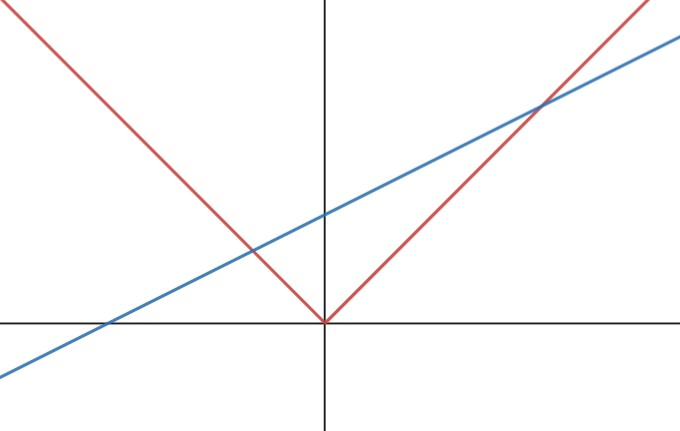
\includegraphics[width=0.3\linewidth]{bonfa_19} $\quad$
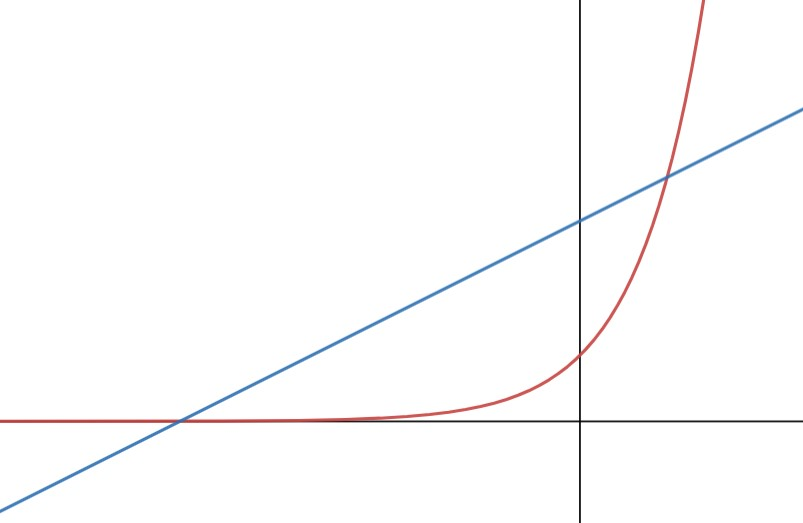
\includegraphics[width=0.3\linewidth]{bonfa_20}
\caption{Funzione modulo (convessa) a sinistra e logaritmo (concava) a destra}
\end{figure}
\FloatBarrier


\begin{defn}
Due numeri $p, q \geq 1$ sono \textbf{esponenti coniugati} se $\dfrac{1}{p} + \dfrac{1}{q} = 1$, con la convenzione che $\dfrac{1}{\infty}=0$.
\end{defn}

\begin{rem}
Prendendo due esponenti coniugati la concavità della funzione logaritmo può essere espressa come
$$
\log\left(\frac{x}{p}+\frac{y}{q}\right)\geq \frac{\log x}{p}+\frac{\log y}{q}
$$
\end{rem}

\begin{thm}[Disuguaglianza di Young]$\\$
Siano $p, q$ esponenti coniugati. Allora $\forall a, b > 0$ vale
\begin{equation*}
ab\leq\frac{a^{p}}{p} + \frac{b^{q}}{q}
\end{equation*}
\end{thm}

\begin{proof}
La dimostrazione si basa sulle proprietà del logaritmo:
$$
\log(ab)=\log(a)+\log(b)=\frac{\log a^p}{p}+\frac{\log b^q}{q}\leq \log\left(\frac{a^p}{p}+\frac{b^q}{q}\right)
$$
Dato che il logaritmo è una funzione crescente posso semplificarlo e ottenere così la tesi.
\end{proof}

\begin{thm}[Disuguaglianza di Holder]$\\$
Sia $A\subseteq\RR^n$ misurabile e siano $p,q\in[1,+\infty]$ coniugati. Se $f\in L^p(A)$ e $g\in L^q(A)$ allora $fg\in L^1(A)$ e
\begin{equation*}
\int_A | f(x) g(x)| \dx=\Vert fg \Vert_1 \leq \Vert f \Vert_{p}\cdot \Vert g \Vert_{q}
\end{equation*}
\end{thm}

\begin{proof}
Dimostriamo prima l'asserto nel caso $p=1$ e $q=\infty$ (la dimostrazione con $q=1$ e $p=\infty$ è del tutto analoga).

Abbiamo $f\in L^1$ e $g\in L^{\infty}$. Per definizione di norma infinito abbiamo 
$$
|g(x)| \leq \Vert g \Vert_{\infty} \qquad\qquad\text{q.o. in }x
$$
e dunque
$$
\int_A |f(x) g(x)| \dx \stackrel{\mathrm{CS}}{\leq} \int_A |f(x)|\cdot|g(x)|\dx\leq \Vert g \Vert_{\infty}\cdot \int_A |f(x)| \dx = \Vert g \Vert_{\infty}\cdot \Vert f \Vert_{1}
$$

Possiamo passare a dimostrare l'asserto per due generici $1<p,q<\infty$. 

Per semplicità consideriamo dapprima due funzioni $\widetilde{f}\in L^p$ e $\widetilde{g}\in L^q$ tali che $\Vert \widetilde{f}\Vert_p=1$ e $\Vert \widetilde{g}\Vert_q=1$. In questo modo per la disuguaglianza di Young si ha
\begin{align*}
\int_A | \widetilde{f}(x) \widetilde{g}(x)| \dx&\leq \int_A \left(\frac{|\widetilde{f}(x)|^p}{p}+\frac{|\widetilde{g}(x)|^q}{q} \right)\dx \\
&=\left(\frac{\Vert \widetilde{f}\Vert_p^p}{p}+\frac{\Vert \widetilde{g}\Vert_q^q}{q}\right) \\
&=\frac{1}{p}+\frac{1}{q} \\
&=1\left(=\Vert \widetilde{f}\Vert_p\cdot \Vert \widetilde{g}\Vert_q\right)
\end{align*} 

Ma allora il caso generale (con norme non necessariamente unitarie) è banale da verificare:
\begin{gather*}
f(x)=\frac{f(x)}{\Vert f \Vert_{p}} \cdot \Vert f \Vert_{p} = \widetilde{f}(x)\cdot \Vert f \Vert_{p} \\
g(x)=\frac{g(x)}{\Vert g \Vert_{q}} \cdot \Vert g \Vert_{q} = \widetilde{g}(x)\cdot \Vert g \Vert_{q} \\
\Longrightarrow \int_A | f(x) g(x)| \dx \stackrel{\mathrm{CS}}{\leq}\Vert f \Vert_{p}\cdot \Vert g \Vert_{q} \cdot \int_A | \widetilde{f}(x) \widetilde{g}(x)| \dx \leq \Vert f \Vert_{p}\cdot \Vert g \Vert_{q}
\end{gather*}
\end{proof}

Conseguenze della disuguaglianza di Holder:
\begin{itemize}
    \item Se $A\subset\RR^n$ è un insieme di \underline{misura finita} e $1\leq p<q\leq+\infty$ allora vale l'inclusione $L^q(A)\subset L^p(A)$ e inoltre
    $$
    \Vert f \Vert_p\leq |A|^{\frac{1}{p}-\frac{1}{q}}\Vert f\Vert_q \qquad \qquad \forall f\in L^q(A) 
    $$
    \begin{rem}
    L'ipotesi di misura finita è indispensabile: infatti se ad esempio $f\equiv 1$ abbiamo $f\in L^\infty(\RR)$ ma $f\notin L^p(\RR)$ per ogni $1\leq p<\infty$.
    \end{rem}

    \item Se $A\subset\RR^n$ è un insieme di misura finita allora per ogni funzione misurabile $f$ si ha
    $$
    \lim_{p\to\infty}\Vert f\Vert_p=\Vert f\Vert_{\infty}
    $$

    \item Permette di dimostrare che $L^2$ è uno spazio di Hilbert (pensandoci, l'unico esponente coniugato con se stesso è proprio $p=2$).
\end{itemize}

\begin{thm}[Disuguaglianza di Minkowski]$\\$
Siano $p \geq 1, f\in L^{p}, g\in L^{p}$. Allora
\begin{equation*}
(f + g) \in L^{p} \ \ \text{e} \ \ \Vert f + g \Vert_{p} \leq \Vert f \Vert_{p} + \Vert g \Vert_{p}
\end{equation*}
\end{thm}
\begin{proof}
\begin{align*}
\Vert f + g \Vert^{p}_{p} & = \int | f(x) + g(x)|^{p} \dx\\
 & = \int | f(x) + g(x)|^{p - 1}| f(x) + g(x)| \dx\\
 & \leq \int \underbrace{| f(x) + g(x)|^{p - 1}}_{A}\underbrace{| f(x)|}_{B} \dx + \int \underbrace{| f(x) + g(x)|^{p - 1}}_{C}\underbrace{| g(x)|}_{D} \dx
\end{align*}
Consideriamo $h(x) = A$
\begin{equation*}
[h(x)]^{q} = [h(x)]^{\frac{p}{p - 1}} = | f(x) + g(x)|^{p}
\end{equation*}
Sappiamo già, per dimostrazione precedente, che $(f + g) \in L^{p}$, allora $h\in L^{q}$. Usiamo la disuguaglianza di Holder su $A\in L^{q}, B\in L^{p}$ e $C\in L^{q}, D\in L^{p}$. Otteniamo
\begin{align*}
\Vert f + g \Vert^{p}_{p} & \leq \Vert f \Vert_{p}\left \Vert \ | f + g|^{p - 1} \ \right \Vert_{q} + \Vert g \Vert_{p}\left \Vert \ | f + g|^{p - 1} \ \right \Vert_{q}
\end{align*}
osserviamo il termine che si presenta due volte
\begin{align*}
\left \Vert \ | f + g|^{p - 1} \ \right \Vert_{q} & = \left(\int | f(x) + g(x)|^{(p - 1) q} \dx\right)^{1/q}\\
 & = \left(\int | f(x) + g(x)|^{p} \dx\right)^{1/q}\\
 & = \left(\Vert f + g \Vert^{p}_{p}\right)^{1/q}\\
 & = \Vert f + g \Vert^{p/q}_{p}\\
 & = \Vert f + g \Vert^{p - 1}_{p}
\end{align*}
allora
\begin{gather*}
\Vert f + g \Vert^{p}_{p} \leq \Vert f \Vert_{p} \Vert f + g \Vert^{p - 1}_{p} + \Vert g \Vert_{p} \Vert f + g \Vert^{p - 1}_{p}\\
\implies \ \ \Vert f + g \Vert_{p} \leq \Vert f \Vert_{p} + \Vert g \Vert_{p}
\end{gather*}
\end{proof}


\chapter{Distribuzioni}

Le distribuzioni non sono altro che una generalizzazione, davvero molto più ampia e flessibile, del concetto di funzioni. C'è sempre un prezzo da pagare, che in questo caso è una maggiore complessità nella definizione. Dunque, prima di arrivare alla definizione di distribuzione dobbiamo fare alcuni passaggi preliminari.

\section{Spazio delle funzioni \texorpdfstring{$\Cc^\infty$}{C}}

Parliamo di funzioni $f\in\Cc^\infty(A)$, con $A\subset\RR$ aperto (si può generalizzare al caso $\RR^n$ in maniera del tutto analoga).

\begin{defn}[Supporto di una funzione]$\\$
Sia $A\subset\RR$ aperto e sia $f\in\Cc^\infty(A)$. Chiamiamo supporto di $f$ e lo indichiamo con
\begin{equation*}
\supp f = \overline{\{x\in A\ :\ f(x) \neq 0\}}
\end{equation*}
la chiusura dell'insieme dei punti dove la funzione non si annulla.
\end{defn}

\begin{defn}
Definiamo
\begin{equation*}
\Dc(A)=\left\{f\in\Cc^\infty\ :\ \supp f \text{ è compatto in }A\right\}
\end{equation*}
\end{defn}
In sostanza, $\Dc(A)$ contiene quelle funzioni regolari su $A$ che si annullano prima di raggiungere il bordo $\partial A$ o prima di raggiungere l'infinito (se $A$ è illimitato): deve quindi valere che $\supp f\subset A$.

\begin{exa}
Fare esempi di funzioni $f\in\Dc$ non è per niente banale, e già questo è indice del fatto che lo spazio $\Dc$ sia uno spazio estremamente ``piccolo'', ovvero contenente poche funzioni.

\begin{equation*}
f(x)=\begin{cases}
e^{\frac{1}{x^2-1}} &|x|<1 \\
0 &\text{altrove}
\end{cases}
\qquad \in \Dc\left((-2,2)\right)
\end{equation*}

\fg{0.5}{esempioFunzioneD}

Tale funzione assomiglia ad una gaussiana, ma fuori $[-1,1]$ si annulla.

Non è banale che sia $C^{\infty}$ nei punti $ - 1, 1$, ma si può dimostrare.

Vediamo un altro esempio:

\begin{equation*}
f(x)=1\notin\Dc(0,1)\text{ perché }\supp f=[0,1]\not\subset A=(0,1)
\end{equation*}

Intuiamo che nessuna funzione elementare può appartenere a $\Dc$.

\end{exa}

Abbiamo quindi capito che solo poche funzioni appartengono allo spazio $\Dc$ proprio perché vengono richieste delle condizioni molto forti; questo però garantisce ottime proprietà. Una tra queste è:

\begin{thm}
\label{teo_denso}
Sia $A\subset \RR^n$ aperto. e sia $p\in[1,\infty)$ ($p=\infty$ escluso!). Allora $\forall p$ lo spazio $\Dc(A)\subset L^p(A)$ ed è ivi denso, e cioè
\begin{equation*}
\forall f\in L^p(A),\ \forall \Ec>0\ \ \exists\varphi_\Ec\in\Dc(A)\ \text{tc}\ \Vert f-\varphi_\Ec\Vert_p<\Ec
\end{equation*}
\end{thm}
Tale teorema afferma che è sempre possibile approssimare (nel senso della norma di $L^p$) una funzione $\phi\in L^p$ con una funzione $f\in\Dc$.


\section{Spazio delle funzioni localmente \texorpdfstring{$L^p$}{C}}

\begin{defn}
Sia $A\subset\RR^n$ aperto e sia $1\leq p\leq\infty$. Si indica con $L^{p}_{\loc}(A)$ lo spazio
\begin{equation*}
L^{p}_{\loc}(A)=\left\{f\in L^p(K)\ \ \forall K\text{ compatto}\subset A\right\}
\end{equation*}
(il pedice ``loc'' sta per locale)
\end{defn}
Tale spazio contiene tutte le funzioni $L^p(A)$ e inoltre anche quelle funzioni non $p$-integrabili in $A$ ma in un $K$ (chiuso) e limitato contenuto in $A$. Dunque le $f\in L^{p}_{\loc}(A)$ sono quelle che hanno un \textit{buon comportamento} all'interno di $A$, ma per le quali non si hanno informazioni vicino a $\partial A$.

\begin{exa}
\begin{equation*}
f(x)=x^{1/3}\in L^1_{\loc}(\RR)\text{ ma }\notin L^1(\RR)
\end{equation*}
\begin{equation*}
f(x)=\frac{1}{x}\in L^1_{\loc}(0,\infty)\text{ ma }\notin L^1(0,\infty)
\end{equation*}
\end{exa}

Pur non essendo possibile definire sullo spazio $L^p_{\loc}$ una norma naturale è tuttavia possibile introdurre una nozione di convergenza, con l'accortezza che, essendo $L^p_{\loc}$ più ``grande'' di $L^p$, la convergenza in $L^p_{\loc}$ sarà più ``debole'' rispetto a quella in $L^p$.

\begin{defn}
Sia $\{f_n\}$ una successione in $L^p_{\loc}$(A), con $p\geq 1$. Si dice che $f_n\xrightarrow[]{L^p_{\loc}(A)}f$ se $f_n\xrightarrow[]{L^p(K)}f$ per ogni $K$ compatto $\subset A$, cioè se
\begin{equation*}
\int_K |f_n-f|^p\,\dx\to 0\qquad \forall K\subset A
\end{equation*}
\end{defn}

\begin{thm}
\label{per_dim_delta}
Sia $A\subset\RR^n$ aperto e sia $f\in L^1_{\loc}(A)$ tale che
\begin{equation*}
\int_A f\varphi=0\qquad \forall \varphi\in\Dc(A)
\end{equation*}
Allora $f=0$ q.o. in $A$.
\end{thm}


\section{Distribuzioni}

Sullo spazio $\Dc(A)$ introduciamo la seguente nozione di convergenza:
\begin{defn}
Siano $A\subset\RR$ aperto, $\{f_n\}\subset\Dc(A)$ e $f\in\Dc(A)$. Si dice che 
\begin{equation}
\label{conv_1_distrib}
f_n\xrightarrow[]{\Dc(A)}f
\end{equation} 
se valgono le seguenti condizioni:
\begin{enumerate}
    \item [(i)] esiste $K\subset A$ compatto tale che $\supp f_n\subset K$ per ogni $n\in\NN$
    \item [(ii)] $f_n^{(\alpha)}\xrightarrow[]{}f^{(\alpha)}$ uniformemente in $A$ per ogni indice $\alpha$.
\end{enumerate}
\end{defn}
Questa convergenza è molto ``forte'', in linea col fatto che $\Dc$ è uno spazio molto ``piccolo''.

A questo punto possiamo definire lo spazio delle distribuzioni.

\begin{defn}[Distribuzione]$\\$
Una distribuzione su $A$ aperto in $\RR$ è un funzionale lineare e continuo su $\Dc(A)$. Quindi lo spazio delle distribuzioni, che viene indicato con $\Dc'(A)$, è il duale di $\Dc(A)$.
\end{defn}

\begin{rem}
È bene sottolineare che il codominio di una distribuzione, in quanto funzionale, è $\RR\,$!!
\end{rem}

Come detto a inizio capitolo, tale definizione risulta molto complessa poiché molto astratta. Cerchiamo di capire come tutto questo possa stare in piedi, soprattutto come generalizzazione del concetto di funzione.

Sia $\Lambda:\Dc(A)\to\RR$ una distribuzione $\in\Dc'(A)$. Allora:
\begin{itemize}
    \item $\Lambda$ è lineare, cioè
    \begin{equation*}
    \Lambda(a_1\varphi_1+a_2\varphi_2)=a_1\Lambda(\varphi_1)+a_2\Lambda(\varphi_2)\qquad \forall \varphi_{1,2}\in\Dc(A),\ \forall a_{1,2}\in\RR
    \end{equation*}
    \item $\Lambda$ è continuo (nel senso di \eqref{conv_1_distrib}), cioè
    \begin{equation}
    \label{conv_2_distrib}
    \Lambda(\varphi_n)\xrightarrow[]{}\Lambda(\varphi)\qquad \forall \{\varphi_n\}\subset\Dc(A)\text{ tc }\varphi_n\xrightarrow[]{\Dc(A)}\varphi
    \end{equation}
    \textbf{N.B.} Il numero reale $\Lambda(\varphi)$ verrà indicato con $(\Lambda,\varphi)$ per motivi che saranno ben chiari più avanti.
    \item Per ogni $u\in L^1_{\loc}$ associamo la distribuzione $\Lambda_u$ definita da
    \begin{equation*}
    \boxed{(\Lambda_u,\varphi):=\int_A u\varphi \qquad \forall \varphi\in\Dc(A)}
    \end{equation*}
    \begin{proof}
    Dobbiamo verificare che la definizione sia ben posta, ovvero che $(\Lambda_u,\varphi)$ sia effettivamente un funzionale lineare e continuo.
    \begin{itemize}
        \item [$\triangleright$] $\varphi\in\Dc(A)$ cioè $\varphi\in\Cc^\infty$ e $\supp\varphi$ è compatto. Detto $K\subset A$ un compatto che contiene $\supp\varphi$, tra le tante cose si ha che $\varphi$ si annulla al di fuori di $K$ e che $\varphi$ ammette massimo finito in $K$. Allora, ricordando che per ipotesi $u\in L^1_{\loc}$ (quindi è integrabile su qualsiasi $K\subset A$ secondo Lebesgue), si ha
        \begin{equation*}
        \int_A |u\varphi|=\int_K |u\varphi| \leq \max|\varphi|\cdot\int_K |u|<+\infty\ \Rightarrow\ \int_A |u\varphi|\text{ è int. secondo Lebesgue}
        \end{equation*}
        e dunque la definizione è quanto meno corretta: $\Lambda_u$ è un funzionale che, applicato a $\varphi$, restituisce un numero reale.
        \item [$\triangleright$] $\Lambda_u$ è lineare poiché
        \begin{equation*}
        (\Lambda_u,a_1\varphi_1+a_2\varphi_2)=\int_A u (a_1\varphi_1+a_2\varphi_2)=a_1(\Lambda_u,\varphi_1)+a_2(\Lambda_u,\varphi_2)
        \end{equation*}
        \item [$\triangleright$] Dobbiamo ora dimostrare la continuità del funzionale, ovvero, come fatto in \eqref{conv_2_distrib}, che
        \begin{equation*}
        \{\varphi_n\}\text{ tc }\varphi_n\xrightarrow[]{\Dc(A)}\varphi\ \Rightarrow\ (\Lambda_u,\varphi_n)\xrightarrow[]{}(\Lambda_u,\varphi)
        \end{equation*}
        Questo può essere inteso come $(\Lambda_u,\varphi_n-\varphi)\xrightarrow[]{}0$ nel vero senso di limite per numeri reali, e dunque la cosa più comoda è dimostrare che $\int_A u(\varphi_n-\varphi)\xrightarrow[]{}0$ andandone a maggiorare il modulo. \\
        Prima di fare ciò ricordiamo le ipotesi di lavoro: $\varphi$ e $\varphi_n$ stanno in $\Dc(A)$ dunque esiste un compatto $K\subset A$ che contiene $\supp\varphi$ e $\supp\varphi_n$ per ogni $n$; $\varphi_n^{(\alpha)}\to\varphi^{(\alpha)}$ uniformemente $\forall n,\alpha$ e quindi in particolare per $\alpha=0$ si ha che $\max|\varphi_n-\varphi|\to 0$; infine, $u\in L^1_{\loc}$ quindi è integrabile in $K$ secondo Lebesgue. \\
        Allora:
        \begin{equation*}
        \int_A |u(\varphi_n-\varphi)|=\int_K |u(\varphi_n-\varphi)|\leq \int_K |u|\cdot |\varphi_n-\varphi|\leq \max|\varphi_n-\varphi|\cdot \int_K |u| \to 0
        \end{equation*}
    \end{itemize}
    \end{proof}
    \item La mappa $u\mapsto\Lambda_u$ è iniettiva (ma non suriettiva), cioè prese $u,v\in L^1_{\loc}$ con $u\neq v$ si ha che anche $\Lambda_u\neq\Lambda_v$. Infatti
    \begin{equation*}
    (u-v,\varphi)=\int_A (u-v)\varphi=0\ \ \ \forall\varphi\in\Dc(A)\quad \Leftrightarrow\quad u=v\ \text{ q.o.}
    \end{equation*}
\end{itemize}

Grazie a questi quattro punti abbiamo capito che ad ogni funzione $u\in L^1_{\loc}(A)$ si può associare un funzionale $\Lambda_u\in\Dc'(A)$ lineare e continuo secondo la definizione di $(\Lambda_u,\varphi)$, con $\varphi\in \Dc(A)$. Abbiamo quindi instaurato la corrispondenza 
\begin{equation*}
u\in L^1_{\loc}\mapsto \Lambda_u\in\Dc'
\end{equation*}
Sappiamo già che lo spazio $L^1_{\loc}$ è molto ``grande'', nel senso che contiene tante funzioni; vogliamo quindi capire se lo spazio delle distribuzioni è ancora più ``grande'', cioè
\begin{equation*}
L^1_{\loc}(A)\overset{\underset{\mathrm{??}}{}}{\subset}\Dc'(A)
\end{equation*}
Per dire questo basta trovare una distribuzione che non appartiene a $L^1_{\loc}$.

\begin{rem}
Da qui in poi, ogni qual volta si vorrà snellire la notazione si identificherà la dualità $(\Lambda_u,\varphi)$ semplicemente con $(u,\varphi)$. Scriveremo dunque ``intendendo $u$ come distribuzione'', sottointendendo il fatto che a ogni $u\in L^1_{\loc}$ sia possibile associare la distribuzione $\Lambda_u$.
\end{rem}

\subsection{La delta di Dirac}

Dato $y\in A\subset\RR$ aperto, si consideri il funzionale $\delta_y\in\Dc'(A)$ definito da
\begin{equation*}
\delta_y:\Dc(A)\to\RR\quad\qquad (\delta_y,\varphi):=\varphi(y)\in\RR
\end{equation*}
La delta di Dirac serve quindi per estrarre il valore di una funzione in un punto, ed è in realtà il punto di partenza per lo sviluppo della teoria delle distribuzioni.

Verifichiamo che tale funzionale sia davvero una distribuzione, cioè che sia lineare e continuo:
\begin{align*}
(\delta_y,a_1\varphi_1+a_2\varphi_2)&\overset{\underset{\mathrm{def}}{}}{=}a_1\varphi_1(y)+a_2\varphi_2(y)=a_1(\delta_y,\varphi_1)+a_2(\delta_y,\varphi_2) \\
(\delta_y,\varphi_n-\varphi)&\overset{\underset{\mathrm{def}}{}}{=}\varphi_n(y)-\varphi(y)\to0\qquad \qquad \text{con }\varphi_n\xrightarrow[]{\Dc}\varphi
\end{align*}

Bene, vogliamo ora dimostrare che non esiste $u\in L^1_{\loc}(A)$ tale che
\begin{equation*}
(\delta_y,\varphi)=\int_A u\varphi\qquad \forall\varphi\in\Dc(A)
\end{equation*}

\begin{proof}
Suppiamo per assurdo che questa $u\in L^1_{\loc}(A)$ esista. Allora, per ogni $\varphi\in\Dc(A)$ tale che $y\notin\supp\varphi$ (e cioè $\varphi(y)=0$) si ha
\begin{equation*}
\int_A u\varphi=(\delta_y,\varphi)=\varphi(y)=0
\end{equation*}
Grazie al teorema (\ref{per_dim_delta}) applicato all'insieme aperto $A\setminus\{y\}$ si conclude che $u=0$ q.o. in $A$. Ma questo porta a dire che
\begin{equation*}
\varphi(y)=(\delta_y,\varphi)=\int_Au\varphi=0\qquad \forall \varphi\in\Dc(A)
\end{equation*}
che è ovviamente assurdo perché le funzioni di $\Dc(A)$ non sono necessariamente nulle in $y$.
\end{proof}

Possiamo quindi affermare con certezza che $\Dc'$ è un'ampia estensione di $L^1_{\loc}$. Questo potevamo anche dedurlo a livello intuitivo dal concetto di dualità: più uno spazio è ``piccolo'' più il suo duale è ``grande''. Infatti, lo spazio $\Dc$ è più ``piccolo'' di $L^1_{\loc}$ e dunque il suo duale, $\Dc'$, sarà conseguentemente più ``grande'' di $L^1_{\loc}$.

\subsection{Convergenza di una distribuzione}

Anche sullo spazio $\Dc'(A)$ è possibile introdurre una convergenza.

\begin{defn}[Convergenza nel senso delle distribuzioni]$\\$
Siano $A\subset\RR$ aperto, $\{\Lambda_n\}\subset\Dc'(A)$ e $\Lambda\in\Dc'(A)$. Si dice che
\begin{equation}
\label{conv_3_distrib}
\Lambda_n\xrightarrow[]{\Dc'(A)}\Lambda
\end{equation}
se
\begin{equation*}
(\Lambda_n,\varphi)\to(\Lambda,\varphi)\qquad \forall\varphi\in\Dc(A)
\end{equation*}
(limite nel senso dei numeri reali!)
\end{defn}
Tale definizione è in perfetta simmetria con la definizione di continuità \eqref{conv_2_distrib}:
\begin{align*}
\varphi_n\xrightarrow[]{\Dc(A)}\varphi\quad&:\quad (\Lambda,\varphi_n)\to(\Lambda,\varphi)\\
\Lambda_n\xrightarrow[]{\Dc'(A)}\Lambda\quad&:\quad(\Lambda_n,\varphi)\to(\Lambda,\varphi)
\end{align*}
Tali definizioni sono una il duale dell'altra, e capiamo quindi perché si preferisce la notazione $(\Lambda,\varphi)$ a $\Lambda(\varphi)$.

\textit{Esempio.} Si consideri la successione $\{u_n\}\in L^1(\RR)$ definita da
\begin{equation*}
u_n(x)=\begin{cases}
n&x\in[0,1/n] \\
0&\text{altrove}
\end{cases}
\end{equation*}
Notiamo subito che 
\begin{equation*}
\Vert u_n\Vert_{L^1}=\int_\RR u_n(x)\dx=1
\end{equation*}
Ma a cosa converge $u_n$ nel senso delle distribuzioni?
\begin{equation*}
(u_n\varphi)=\int_\RR u_n(x)\varphi(x)\dx=\int_0^{1/n} n\varphi(x)\dx
\end{equation*}
Applicando il Teorema della media integrale
\begin{equation*}
\frac{1}{b-a}\int_a^b f(x)\dx=f(x^*) \qquad \text{con }x^*\in[a,b]
\end{equation*}
possiamo dire che
\begin{equation*}
\int_0^{1/n} n\varphi(x)\dx=\frac{1}{1/n-0}\int_0^{1/n}\varphi(x)\dx=\varphi(x_n)\qquad \text{con }x_n\in\left[0,\frac{1}{n}\right]
\end{equation*}
E quindi
\begin{equation*}
(u_n,\varphi)=\varphi(x_n)\xrightarrow[]{n\to+\infty}\varphi(0)\quad\Rightarrow\quad u_n\xrightarrow[]{\Dc'(\RR)}\delta_0
\end{equation*}
Tale esempio mostra come si può interpretare matematicamente la delta di Dirac: è il limite (nel senso delle distribuzioni) di una successione di funzioni di $L^1$ che ``tende a concentrare la massa'' nel centro della delta. Grazie a tale osservazione è banale fornire un altro esempio, quello della \underline{gaussiana}:
\begin{equation*}
u_n=e^{-\frac{x^2}{2\sigma_n}}\xrightarrow[]{\sigma_n\to0}\delta_0
\end{equation*} 


\subsection{Supporto di una distribuzione}

È possibile estendere la nozione di supporto, precedentemente introdotto per le funzioni, anche alle distribuzioni.

\begin{defn}
Sia $A\subset\RR$ aperto e sia $\Lambda\in\Dc'(A)$. Se $\omega$ è un sottoinsieme aperto di $A$ diremo che la distribuzione $\Lambda$ si annulla in $\omega$ se $(\Lambda,\varphi)=0$ per ogni $\varphi\in\Dc(\omega)$.\\
A questo punto ha senso introdurre $\Omega$ definito come l'unione di tutti gli aperti $\omega\subset A$ sui quali $\Lambda$ si annulla:
\begin{equation*}
\Omega:=\bigcup_{\Lambda\text{ nulla}}\omega\qquad\text{ (l'unione di aperti è ancora un'aperto!)}
\end{equation*}
Allora si definisce supporto di $\Lambda$ il complementare di $\Omega$:
\begin{equation*}
\boxed{\supp\Lambda:=\Omega^c}
\end{equation*}
\end{defn}
Facciamo qualche osservazione:
\begin{itemize}
    \item Tale definizione è perfettamente compatibile con la precedente definizione di supporto, nel senso che se $u\in\Cc^0(A)\cap L^1_{\loc}(A)$ allora l'insieme
    \begin{equation*}
    \supp u=\overline{\{x\in A\ :\ u(x)\neq0\}}
    \end{equation*}
    coincide con il supporto della distribuzione associata a $u$.
    \item Tale definizione permette di dare un significato al supporto di una funzione $L^p$. Ricordiamo che gli elementi di $L^p$ non sono funzioni ma classi di equivalenza di funzioni (funzioni uguali q.o.) e quindi l'unica definizione di supporto che ha davvero senso è quella nel senso delle distribuzioni.
    \item  Le delta di Dirac sono distribuzioni a supporto compatto: $\supp\delta_y=\{y\}$.
    \item Anche le funzioni $L^1(\RR^n)$ a supporto compatto sono distribuzioni a supporto compatto.
\end{itemize}

\subsection{Derivata in senso distribuzionale}

Prima di vedere la definizione di derivata cerchiamo di capire il percorso che ha portato ad essa.

Sia $A\subset \RR$ aperto e sia $f\in\Cc^1(A)$. Intendendo $f$ come distribuzione, $\forall\varphi\in\Dc(A)$
\begin{equation*}
(f',\varphi):=\int_Af'(x)\varphi(x)\dx\overset{\underset{\mathrm{pp}}{}}{=}\left[f(x)\varphi(x)\right]_{\partial A}-\int_A f(x)\varphi'(x)\dx\overset{\underset{\varphi\in\Dc}{}}{=}-\int_Af(x)\varphi'(x)\dx=:-(f,\varphi')
\end{equation*}

Se si potesse estendere tale proprietà, dedotta dal Teorema di integrazione per parti e dalla definizione di funzioni $\Cc^\infty$ a supporto compatto, alle distribuzioni potremmo benissimo dare la seguente:

\newpage

\begin{defn}[Derivata di una distribuzione]$\\$
Sia $\Lambda \in \Dc'(A)$ una distribuzione. Definiamo la sua derivata $\Lambda'\in \Dc'(A)$ la distribuzione data da
\begin{equation*}
\boxed{(\Lambda', \varphi) = - (\Lambda, \varphi')}\qquad\forall\varphi\in\Dc(A)
\end{equation*}
\end{defn}
Ora controlliamo che effettivamente tale estensione sia coerente:
\begin{itemize}
\item $\Lambda': \Dc(A)\rightarrow \RR$, ben definita!
\item $(\Lambda', a_{1} \varphi_{1} + a_{2} \varphi_{2}) = a_{1}(\Lambda', \varphi_{1}) + a_{2}(\Lambda', \varphi_{2})$, lineare!
\item $(\Lambda', \varphi_{n})\rightarrow (\Lambda', \varphi)\ \ \forall \varphi_{n}\xrightarrow[]{\Dc(A)} \varphi$, continua!
\end{itemize}

\begin{rem}
Se $u\in L^1_{\loc}$ è derivabile in senso tradizionale allora la sua derivata coincide con quella tradizionale. Viceversa, $u$ potrebbe anche non essere derivabile in senso tradizionale, ma potremo sempre scrivere $u'$ intendendo la derivata in senso distribuzionale, poiché questa esiste sempre (tra poco lo scoprirai).
\end{rem}

\textit{Esempio importante.} Consideriamo la funzione
\begin{equation*}
u(x) =
\begin{cases}
x & x \geq 0\\
0 & x < 0
\end{cases}
\end{equation*}
\fg{0.5}{rampa}
Tale funzione è continua su $\RR$ e perciò $L^1_{\loc}(\RR)$, ma presenta un punto angoloso nell'origine dunque non è derivabile in senso tradizionale. Intendendo $u$ come distribuzione, $\forall\varphi \in \Dc(\RR)$ si ha
\begin{equation*}
(u', \varphi) = - (u, \varphi') = - \int_{\RR} u(x) \varphi'(x) \dx=- \int_0^{+\infty} u(x) \varphi'(x) \dx = - \int^{M}_{0} x\varphi'(x) \dx
\end{equation*}
dove $M$ è il primo valore tale che $\varphi(M)=0$. Integrando ancora per parti si ha
\begin{equation*}
- \int^{M}_{0} x\varphi'(x) \dx =-M\cdot\cancel{\varphi(M)}+\cancel{0}\cdot\varphi(0)+\int^{M}_{0} \varphi (x) \dx = \int^{M}_{0} \varphi (x) \dx=: \int_\RR H(x) \varphi (x) \dx = (H, \varphi)
\end{equation*}
dove $H(x)$ è la \textbf{funzione di Heaviside}
\begin{equation*}
H(x) =
\begin{cases}
1 & x \geq 0\\
0 & x < 0
\end{cases}
\end{equation*}
intesa come distribuzione.

Allora $\boxed{\text{la derivata } u'\text{ di } u\text{ in senso distribuzionale è }H}$.

Sembra che non abbiamo fatto granché se non togliere di mezzo un punto angoloso: spingiamoci oltre e deriviamo la funzione di Heaviside, che non è nemmeno continua.
\begin{align*}
(H', \varphi) & = - (H, \varphi') \ \ \forall \varphi \in \Dc(\RR)\\
 & = - \int_{\RR} H(x) \varphi'(x) \dx = - \int^{+ \infty}_{0} \varphi'(x) \dx\\
 & = \varphi (0) - \lim_{x\rightarrow + \infty} \varphi (x) = \varphi (0) = (\delta_{0}, \varphi)
\end{align*}
Allora $\boxed{\text{la derivata } H'\text{ di } H\text{ in senso distribuzionale è }\delta_0}$.


\section{Funzioni a decrescita rapida e distribuzioni temperate}

Lo spazio delle $\varphi $ è lo spazio delle funzioni test, delle funzioni $C^{\infty}$ a supporto compatto, uno spazio molto stringente. Cerchiamo di allentarlo un po' introducendo un nuovo spazio chiamato \textbf{spazio delle funzioni a decrescita rapida} (o \textbf{spazio di Schwartz}.\footnote{Si noti che si tratta di un matematico differente da quello del teorema sulle derivate seconde, Karl Hermann Amandus Schwarz (1843 - 1921). Qui si parla di Laurent Schwartz (1915 - 2002), medaglia Fields nel 1950.})
\begin{defn}[Spazio delle funzioni a decrescita rapida]$\\$
Diciamo che $f\in \Sc(\RR)$ se 
\begin{equation*}
f\in C^{\infty}\qquad \lim_{x\to\pm\infty}x^nf^{(k)}(x)=0\ \ \forall k, n\in \NN
\end{equation*}
\end{defn}
Esaminando la definizione possiamo capire due cose:
\begin{itemize}
    \item non hanno senso spazi di Schwarz in sottoinsiemi di $\RR$
    \item la seconda condizione, vedi $k=0$, non richiede che $f$ si annulli fuori da un compatto, ma che si annulli più rapidamente di qualsiasi potenza di $x$ (per esempio come la gaussiana $e^{-x^2}$)
\end{itemize}
Dunque questo spazio è ``un pelo'' più grande di $\Dc$:
\begin{equation*}
\Dc(\RR) \subset \Sc(\RR)
\end{equation*}

Come si definisce la convergenza in questo insieme?
\begin{defn}
[Convergenza in $\Sc$]Siano $\{f_{n}\} \subset \Sc(\RR)$ e $f\in\Sc(\RR)$. Diciamo che
\begin{equation}
\label{conv_4_distrib}
f_n\xrightarrow[]{\Sc(\RR)}f
\end{equation}
se $x^{j} f^{(k)}_{n}(x)\xrightarrow{n\rightarrow + \infty} x^{j} f^{(k)}(x)$ uniformemente in $\RR$  $\forall j, k\in \NN$.
\end{defn}
Osserviamo due cose:
\begin{enumerate}
    \item Anche questo non è uno spazio di Banach e non c'è norma.
    \item Se la successione $\{f_n\}$ sta in $\Dc(\RR)$ e converge nel senso di \eqref{conv_1_distrib} allora sta anche in $\Sc(\RR)$ e converge nel senso di \eqref{conv_4_distrib}.
\end{enumerate}

\begin{defn}
[Distribuzione temperata]
Un funzionale $\Lambda : \Sc(\RR)\rightarrow \RR$ lineare e continuo si dice distribuzione temperata, e si scrive $\Lambda\in\Sc'(\RR)$.
\end{defn}
Una distribuzione temperata è anche una distribuzione normale; in altre parole, lo spazio delle distribuzioni temperate $\Sc'(\RR)$ è contenuto in $\Dc'(\RR)$
\begin{equation*}
\Sc'(\RR) \subset \Dc'(\RR)
\end{equation*}
Infatti, se abbiamo due spazi qualsiasi $A\subset B$, i loro duali sono legati da $B'\subset A'$.
\begin{figure}[htpb]
\centering

\tikzset{every picture/.style = {line width = 0.75pt}} %set default line width to 0.75pt

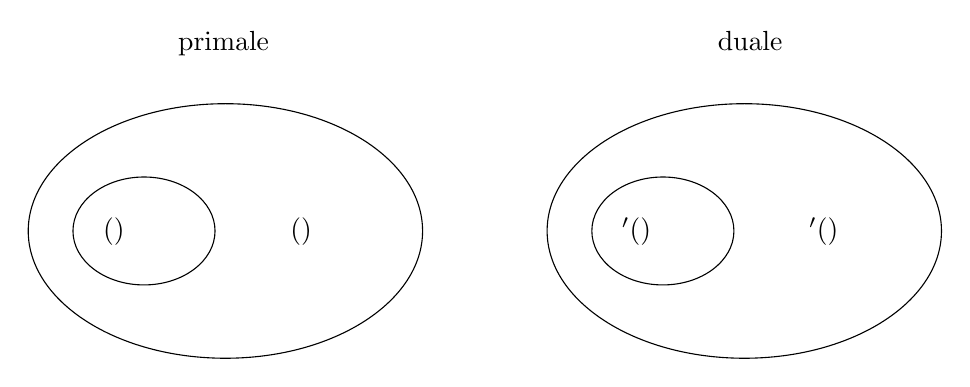
\begin{tikzpicture}[x = 0.75pt, y = 0.75pt, yscale = - 1, xscale = 1]
%uncomment if require: \path (0, 181); %set diagram left start at 0, and has height of 181

%Shape: Ellipse [id: dp7503563455876929]
\draw (80, 108.68) .. controls (80, 74.82) and (122.53, 47.36) .. (175, 47.36) .. controls (227.47, 47.36) and (270, 74.82) .. (270, 108.68) .. controls (270, 142.55) and (227.47, 170) .. (175, 170) .. controls (122.53, 170) and (80, 142.55) .. (80, 108.68) - - cycle;
%Shape: Ellipse [id: dp5108599722199094]
\draw (101.55, 108.68) .. controls (101.55, 94.32) and (116.87, 82.68) .. (135.77, 82.68) .. controls (154.68, 82.68) and (170, 94.32) .. (170, 108.68) .. controls (170, 123.04) and (154.68, 134.68) .. (135.77, 134.68) .. controls (116.87, 134.68) and (101.55, 123.04) .. (101.55, 108.68) - - cycle;
%Shape: Ellipse [id: dp5851131130928555]
\draw (330, 108.68) .. controls (330, 74.82) and (372.53, 47.36) .. (425, 47.36) .. controls (477.47, 47.36) and (520, 74.82) .. (520, 108.68) .. controls (520, 142.55) and (477.47, 170) .. (425, 170) .. controls (372.53, 170) and (330, 142.55) .. (330, 108.68) - - cycle;
%Shape: Ellipse [id: dp4435469561254657]
\draw (351.55, 108.68) .. controls (351.55, 94.32) and (366.87, 82.68) .. (385.77, 82.68) .. controls (404.68, 82.68) and (420, 94.32) .. (420, 108.68) .. controls (420, 123.04) and (404.68, 134.68) .. (385.77, 134.68) .. controls (366.87, 134.68) and (351.55, 123.04) .. (351.55, 108.68) - - cycle;

% Text Node
\draw (205, 101.08) node [anchor = north west][inner sep = 0.75pt] {$\Sc(\RR)$};
% Text Node
\draw (114.77, 101.08) node [anchor = north west][inner sep = 0.75pt] {$\Dc(\RR)$};
% Text Node
\draw (455, 101.08) node [anchor = north west][inner sep = 0.75pt] {$\Dc'(\RR)$};
% Text Node
\draw (364.77, 101.08) node [anchor = north west][inner sep = 0.75pt] {$\Sc'(\RR)$};
% Text Node
\draw (151, 11) node [anchor = north west][inner sep = 0.75pt] [align = left] {primale};
% Text Node
\draw (411, 11) node [anchor = north west][inner sep = 0.75pt] [align = left] {duale};

\end{tikzpicture}
\end{figure}
\FloatBarrier

\begin{exa}
$u(x)=e^x$ è una distribuzione,  ma non è temperata. Invece $\delta_y$ è una distribuzione anche temperata.
\end{exa}

E i concetti di convergenza e derivabilità in $\Sc'$?

\begin{defn}[Convergenza di distribuzioni temperate]$\\$
Siano $\{u_{n}\} \subset \Sc'(\RR)$ e $u\in\Sc'(\RR)$. Diciamo che 
\begin{equation}
u_n\xrightharpoondown[]{\Sc'(\RR)}u
\end{equation}
se per ogni funzione test a decrescita rapida $\varphi \in \Sc(\RR)$, si ha $(u_{n}, \varphi)\rightarrow (u, \varphi)$.
\end{defn}

\begin{defn}[Derivata di distribuzioni temperate]$\\$
Come prima:
\begin{equation*}
(\Lambda',\varphi):=-(\Lambda,\varphi')\qquad \varphi,\varphi'\in\Sc(\RR)
\end{equation*}
\end{defn}

Per concludere: presa una funzione $u\in L^{1}_{\loc}$ è possibile associarle una distribuzione temperata? Valgono questi due risultati.
\begin{thm}
Se $\exists n\in \NN$ tale che $(1 + | x|)^{- n} u(x) \in L^{1}(\RR)$ allora esiste una distribuzione temperata associata $u\in \Sc'(\RR)$.
\end{thm}
\begin{thm}
Se $u\in L^{p}(\RR)$ per un qualsiasi $p\in [1, + \infty]$ allora esiste una distribuzione temperata associata $u\in \Sc'(\RR)$.
\end{thm}


\chapter{La trasformata di Fourier}

La trasformata di Fourier è uno strumento essenziale in molti campi dell'ingegneria, della fisica, della matematica e, più in generale, della ricerca scientifica. Ne tratteremo gli aspetti più teorici e ne descriveremo alcune applicazioni alle equazioni differenziali ordinarie e alle derivate parziali. Tale \textit{trasformata integrale} riveste un ruolo cruciale anche nella teoria degli spazi di Sobolev.


\section{Introduzione}


\begin{defn}
Poniamo
\begin{equation*}
\Cc^{0}_{0}(\RR) = \left\{f:\RR\to\CC\text{ tali che }f\in \Cc^{0}(\RR)\text{ e } \lim_{|x|\rightarrow \infty} f(x) = 0\right\}
\end{equation*}
\end{defn}

Le funzioni in $C^{0}_{0}(\RR)$ sono automaticamente limitate, quindi contenute nello spazio $L^{\infty}(\RR)$ delle funzioni \textit{essenzialmente} limitate:
\begin{equation*}
\Cc_0^0(\RR)\subset L^\infty(\RR)
\end{equation*}

\begin{defn}[Funzione traslata]$\\$
Sia $f\in L^{1}(\RR)$. Per ogni $y\in\RR$ definiamo la funzione traslata
\begin{equation*}
f_{y}(x) = f(x - y)
\end{equation*}
Ovviamente $f_y\in L^1(\RR)$.
\end{defn}

\begin{thm}
\label{per_la_dim_riemann_L}
Sia $f\in L^{1}(\RR)$ e sia $f_y\in L^1(\RR)$ la sua traslata. Allora
\begin{equation*}
\lim\limits_{y\rightarrow 0} \Vert f - f_y \Vert_{L^{1}} = 0
\end{equation*}
\end{thm}


\begin{proof}
Poiché $\Dc(\RR)$ è denso in $L^1(\RR)$ (si veda teorema \ref{teo_denso})
\begin{equation*}
\forall\Ec>0\ \ \exists\varphi\in\Dc(\RR)\text{ tc } \Vert f-\varphi\Vert<\Ec
\end{equation*}
Ovviamente tale risultato vale anche per la traslata
\begin{equation*}
\forall\Ec>0\ \ \exists\varphi_y\in\Dc(\RR)\text{ tc } \Vert f_y-\varphi_y\Vert<\Ec
\end{equation*}
Posto dunque $[a,b]$, con $a\in\RR$ e $b\in\RR$, un generico insieme tale che $\supp\varphi\subset[a,b]$ e $\supp\varphi_y\subset[a,b]$, per l'uniforme continuità di $\varphi$
\begin{equation*}
\forall\Ec>0\ \ \exists\delta>0\text{ tc }|\varphi(x)-\varphi(y)|<\Ec\ \ \forall x,y\text{ tc }|x-y|<\delta
\end{equation*}
che può essere riscritta in
\begin{equation*}
\forall\Ec>0\ \ \exists\delta>0\text{ tc }|\varphi(x)-\varphi(x-y)|<\Ec\ \ \forall y\text{ tc }|y|<\delta
\end{equation*}
Possiamo dunque calcolare $\forall y\text{ tc }|y|<\delta$
\begin{equation*}
\Vert\varphi-\varphi_y\Vert_{L^1}=\int_\RR |\varphi(x)-\varphi_y(x)|\dx=\int_a^b |\varphi(x)-\varphi_y(x)|\dx\leq \Ec(b-a)
\end{equation*}
Ricapitolando, e sottointendendo la norma di $L^1$, abbiamo finora dimostrato che
\begin{equation*}
\forall\Ec>0\ \ \exists\delta>0\text{ tc }\Vert\varphi-\varphi_y\Vert<\Ec(b-a)\ \ \forall y\text{ tc }|y|<\delta
\end{equation*}

Possiamo ora ritornare a $f$:
\begin{align*}
\Vert f - f_y \Vert & = \Vert (f - \varphi) + (\varphi - \varphi_y) + (\varphi_y - f_y) \Vert \\
  &\overset{\underset{\mathrm{tr.}}{}}{\leq} \Vert f - \varphi \Vert + \Vert \varphi - \varphi_y \Vert + \Vert \varphi_y - f_y \Vert \\
 & < \Ec +\Ec(b-a) + \Ec \\
 & =\Ec(b-a+2)
\end{align*}
cioè $ \Vert f - f_y \Vert \to 0$ come volevasi dimostrare.
\end{proof}


\section{Definizione}

\begin{defn}[Trasformata di Fourier]$\\$
Sia $f:\RR\to\CC$ tale che $f\in L^1(\RR)$. Chiamiamo trasformata di Fourier di $f$ la funzione
\begin{equation*}
\hat{f}:\RR\to\CC\qquad\qquad\qquad \hat{f}(z)=\int_\RR e^{-izx}f(x)\dx\qquad x,z\in\RR
\end{equation*}
\end{defn}

\begin{rem}
In alcune trattazioni la definizione di $\hat{f}$ è leggermente diversa: nell'integrale ci può essere $e^{\pm ixz}$ oppure $e^{\pm 2\pi izx}$. La teoria rimane invariata anche se vengono modificate alcune costanti.
\end{rem}

La definizione è ben posta? Certo, infatti 
\begin{equation*}
f\in L^1(\RR) \ \Rightarrow\ \int_\RR |f(x)|\dx<+\infty\ \Rightarrow\ \int_\RR \left| e^{- izx} f(x)\right|\dx<+\infty\ \text{ xk }\left| e^{- izx}\right|=1
\end{equation*}
L'unica cosa che resta da capire è in quale spazio viene trasformato (linearmente) $L^1(\RR)$ da $\hat{f}$. Per rispondere a questa domanda enunciamo il

\begin{thm}[di Riemann-Lebesgue]$\\$ 
Sia $f\in L^{1}(\RR)$. Allora
\begin{equation*}
\boxed{\hat{f} \in C^{0}_{0}(\RR)}\qquad\text{ e }\qquad\boxed{\Vert \hat{f} \Vert_{\infty} \leq \Vert f \Vert_{L^{1}}}
\end{equation*}
\end{thm}

Abbiamo dunque scoperto in che spazio ``vive'' la trasformata di Fourier.

\newpage

\begin{proof}
La dimostrazione si articola in tre punti:
\begin{enumerate}
    \item [$\triangleright$] Continuità: è vero che $z_n\to z\ \Rightarrow\ \hat{f}(z_n)\to\hat{f}(z)$ ??

    Usando il Teorema della convergenza dominata $(\circledast)$ abbiamo banalmente
    \begin{equation*}
    \lim\limits_{n\rightarrow + \infty}\hat{f}(z_n)=\lim\limits_{n\rightarrow + \infty}\int_{\RR} e^{- iz_{n} x} f(x) \dx \overset{\underset{\circledast}{}}{=} \int_{\RR}\lim\limits_{n\rightarrow + \infty} e^{- iz_{n} x} f(x) \dx = \int_{\RR} e^{- izx} f(x) \dx = \hat{f}(z)
    \end{equation*}
    Dobbiamo però verificare se effettivamente le ipotesi di tale teorema sono soddisfatte:
    \begin{equation*}
    \left| e^{- iz_{n} x} f(x)\right|\leq |f(x)|
    \end{equation*}
    Si, sono soddisfatte in quanto $f\in L^1$ (e quindi anche $|f|\in L^1$) e $|f|$ domina l'integranda.


    \item [$\triangleright$] Disuguaglianza delle norme: è vero che $\Vert \hat{f} \Vert_{\infty} \leq \Vert f \Vert_{L^{1}}$ ??

    Usando la proprietà $\displaystyle\left|\int f\right|\leq \int|f|$ possiamo scrivere
    \begin{equation*}
    \left| \hat{f}(z)\right| = \left| \int_{\RR} e^{- ixz} f(x) \dx\right| \leq \int_{\RR}\left| e^{- ixz} f(x)\right| \dx \leq \int_{\RR}| f(x)| \dx = \Vert f \Vert_{L^{1}}
    \end{equation*}
    da cui segue, per la continuità della funzione, la tesi.

    \item [$\triangleright$] Ultimo punto per l'appartenenza a $\Cc_0^0$: è vero che $\lim\limits_{z\to \pm \infty}\hat{f}(z) = 0$ ??

    Ricordiamo che $-1=e^{i\pi}$ e quindi $1=-e^{i\pi}$. Allora
    \begin{equation*}
    \hat{f}(z) = - e^{i\pi}\int_{\RR} e^{- ixz} f(x) \dx = - \int_{\RR} e^{- i(xz - \pi)} f(x) \dx = - \int_{\RR} e^{- iz\left(x - \frac{\pi}{z}\right)} f(x) \dx
    \end{equation*}
    Con il cambio di variabile
    \begin{equation*}
    x' = x - \frac{\pi}{z} \qquad\qquad \dx'=\dx
    \end{equation*}
    otteniamo
    \begin{equation*}
    \hat{f}(z) = - \int_{\RR} e^{- izx'} f\left(x' + \frac{\pi}{z}\right) \dx' = - \int_{\RR} e^{- izx} f\left(x + \frac{\pi}{z}\right) \dx
    \end{equation*}
    dove nell'ultimo passaggio si è ritornati nella variabile $x$ per comodità.

    Scriviamo ora il doppio di $\hat{f}$, prendendo una parte come appena calcolata e l'altra come da definizione:
    \begin{align*}
    2\hat{f}(z) & = \int_{\RR} e^{- ixz} f(x) \dx - \int_{\RR} e^{- izx} f\left(x + \frac{\pi}{z}\right) \dx=\\
     & = \int_{\RR}\left[e^{- ixz} f(x) - e^{- izx} f\left(x + \frac{\pi}{z}\right)\right] \dx=\\
     & = \int_{\RR} e^{- ixz}\left[f(x) - f\left(x + \frac{\pi}{z}\right)\right] \dx
    \end{align*}
    Passiamo al modulo
    \begin{align*}
    2\left| \hat{f}(z)\right| & = \int_{\RR}\left| e^{- ixz}\left[f(x) - f\left(x + \frac{\pi}{z}\right)\right]\right| \dx\\
     & \leq \int_{\RR}\left| f(x) - f\left(x + \frac{\pi}{z}\right)\right| \dx\\
     & = \Vert f - f_{- \pi /z} \Vert_{L^{1}}
    \end{align*}
    Quando $z\rightarrow \pm \infty $ la traslazione $ - \pi /z\rightarrow 0$ per il teorema \ref{per_la_dim_riemann_L} e quindi $\left| \hat{f}(z)\right| \rightarrow 0$ come volevasi dimostrare.
\end{enumerate}
\end{proof}

\textbf{Notazione.} Il teorema di Riemann-Lebesgue suggerisce di introdurre il funzionale
\begin{equation*}
\Fc : L^{1}(\RR)\rightarrow \Cc^{0}_{0}(\RR)
\end{equation*}
lineare e continuo in modo tale da riscrivere la definizione di trasformata di Fourier in
\begin{equation*}
\boxed{\hat{f}(z)=\Fc(f(x),z)=\int_\RR e^{-izx}f(x)\dx}
\end{equation*}


\section{Proprietà}

Possono essere utili le seguenti proprietà.

\begin{thm}
Siano $f,g\in L^1(\RR)$, $\alpha,\beta\in\CC$, e $y\in\RR$. Allora
\renewcommand{\theenumi}{\roman{enumi}}
\begin{enumerate}
    \item linearita
    $$\Fc(\alpha f+\beta g,z)=\alpha\Fc(f,z)+\beta\Fc(g,z)$$
    \item shifting
    $$\Fc(f(x - y), z)=e^{- iyz}\ \Fc(f(x), z)$$
    \item modulazione
    $$\Fc\left(e^{-iyx} f(x), z\right)=\Fc(f(x), z + y)\qquad\text{ oppure }\qquad \Fc\left(e^{iyx} f(x), z\right)=\Fc(f(x), z - y)$$
    \item modulazione
    $$\Fc\left(\cos(z_0x)\,f(x),z\right)=\frac{1}{2}\left[\Fc(f(x),z-z_0)+\Fc(f(x),z+z_0)\right]$$
    \item scaling
    $$\Fc(f(xy),z)=\frac{1}{|y|}\Fc\left(f(x),\frac{z}{y}\right)$$
    \item coniugazione 
    $$\Fc\left(\overline{f(x)}, z\right) = \overline{\hat{f}(- z)}$$
    \item $f$ pari $\implies $ $\hat{f}$ pari
    \item $f$ dispari $\implies $ $\hat{f}$ dispari
    \item $f$ pari e reale $\implies $ $\hat{f}$ pari e reale
    \item $f$ dispari e reale $\implies $ $\hat{f}$ dispari e immaginaria pura
\end{enumerate}
\end{thm}

\begin{proof}$\\$
\renewcommand{\theenumi}{\roman{enumi}}
\begin{enumerate}
\setcounter{enumi}{1}
\item Abbiamo
\begin{align*}
\Fc(f(x - y), z) & = \int_\RR e^{- ixz} f(x - y) \dx= \\
 & = \left\{\text{cambo di var: }x' = x - y\right\}= \\
 & = \int_\RR e^{- i(x'+y)z} f(x') \dx'= \\
 & = e^{- iyz}\int_\RR e^{- ixz} f(x) \dx= \\
 & = e^{- iyz}\ \Fc(f(x), z)
\end{align*}
dove il termine $e^{- iyz}$ prende il nome di cambio di fase.
\item Abbiamo
\begin{equation*}
\Fc\left(e^{-iyx} f(x), z\right)= \int e^{- ixz} e^{-iyx} f(x) \dx= \int e^{- ix(z + y)} f(x) \dx=\Fc(f(x), z + y)
\end{equation*}
e analogamente
\begin{equation*}
\Fc\left(e^{iyx} f(x), z\right) = \int e^{- ixz} e^{iyx} f(x) \dx= \int e^{- ix(z - y)} f(x) \dx = \Fc(f(x), z - y)
\end{equation*}
\end{enumerate}
\end{proof}

Giusto per sbloccarvi dei ricordi dal corso di \textit{Probabilità} citiamo le seguenti proprietà valide per la trasformata di Fourier in $L^1\left(\RR^n\right)$:
\begin{thm}
Siano $f\in L^1\left(\RR^n\right)$, $y\in\RR^n$ e $A$ matrice reale $n\times n$ invertibile. Allora
\renewcommand{\theenumi}{\roman{enumi}}
\begin{enumerate}
    \item $\Fc(f(\mathbf{x}-\mathbf{y}), \mathbf{z})=e^{- i\mathbf{z}\cdot \mathbf{y}}\ \Fc(f(\mathbf{x}), \mathbf{z})$
    \item $\Fc\left(e^{i\mathbf{y}\cdot \mathbf{x}} f(\mathbf{x}), \mathbf{z}\right)=\Fc(f(\mathbf{x}), \mathbf{z}-\mathbf{y})$
    \item $\Fc\left(f\left(A\mathbf{x}\right),\mathbf{z}\right)=\dfrac{1}{\left|\det A\right|}\ \Fc\left(f(\mathbf{x}),A^{-T}\mathbf{z}\right)$
    \item $\Fc\left(\overline{f(\mathbf{x})}, \mathbf{z}\right) = \overline{\hat{f}(-\mathbf{z})}$
    \item $f$ pari $\implies $ $\hat{f}$ pari
    \item $f$ dispari $\implies $ $\hat{f}$ dispari
    \item $f$ pari e reale $\implies $ $\hat{f}$ pari e reale
    \item $f$ dispari e reale $\implies $ $\hat{f}$ dispari e reale
\end{enumerate}
\end{thm}


\section{Derivata}


Vogliamo capire se una trasformata di Fourier è derivabile.
\begin{thm}[Derivata della trasformata]$\\$
Sia $f\in L^{1}$ e sia $g\in L^{1}$ definita da $g(x) = -ixf(x)$. Allora $\hat{f} \in \Cc^{1}$ e
\begin{equation*}
\left(\hat{f}(z)\right)' = \hat{g}(z)\qquad\text{ e analogamente }\qquad \frac{\de}{\dz}\,\Fc(f(x),z)=\Fc(-ixf(x),z)
\end{equation*}
\end{thm}

\begin{rem}
Volendo si può anche prendere $g(x)=xf(x)$ e concludere che
\begin{equation*}
\left(\hat{f}(z)\right)' = -i\,\hat{g}(z)
\end{equation*}
oppure invertendo
\begin{equation*}
\hat{g}(z)=i\left(\hat{f}(z)\right)'
\end{equation*}
\end{rem}

\begin{proof}
Calcoliamo il limite del rapporto incrementale
\begin{align*}
\lim\limits_{h\rightarrow 0}\frac{\hat{f}(z + h) - \hat{f}(z)}{h} & = \lim\limits_{h\rightarrow 0}\frac{1}{h}\left(\int_\RR e^{- ix(z + h)} f(x) \dx - \int_\RR e^{- ixz} f(x) \dx\right)=\\
 & = \lim\limits_{h\rightarrow 0}\int_\RR e^{- ixz}\,\frac{e^{- ixh} - 1}{h}\,f(x) \dx=\\
  & \overset{\underset{(\alpha)}{}}{=}\int_\RR e^{- ixz}\,\underbrace{\lim\limits_{h\rightarrow 0}\frac{e^{- ixh} - 1}{h}}_{=-ix}\,f(x) \dx=\\
 & \overset{\underset{(\beta)}{}}{=} \int_\RR e^{-ixz}(-ixf(x)) \dx=\hat{g}(z)
\end{align*}
dove in $(\alpha)$ possiamo passare al limite sotto il segno di integrale perché in generale
\begin{equation*}
\left| e^{i\lambda} - 1\right| \leq | \lambda |\qquad\text{con }\lambda \in \RR
\end{equation*}
dove per noi $\lambda=-xh$. Rimarchiamo inoltre che in $(\beta)$ l'integrale è ben definito perché per ipotesi $g\in L^1$.
\end{proof}

\begin{thm}[Trasformata della derivata]$\\$
Sia $f\in L^{1} \cap \Cc^{1}$ tale che $f(x)=o(1)$ per $x\to\pm\infty$ e sia $f'\in L^{1}$. Allora
\begin{equation*}
\widehat{\left(f'\right)}(z) = iz\,\hat{f}(z)\qquad\text{ e analogamente }\qquad \Fc\left(\frac{\de}{\dx}\,f(x),z\right)=\Fc\left(f'(x),z\right)=iz\,\Fc(f(x),z)
\end{equation*}
\end{thm}

\begin{proof}
Abbiamo
\begin{align*}
\widehat{\left(f'\right)}(z)&=\int_\RR e^{-izx}f'(x)\dx=\lim_{R\to+\infty}\int_{-R}^Re^{-izx}f'(x)\dx=\\
&\overset{\underset{\mathrm{pp}}{}}{=}\lim_{R\to+\infty}\left( \left[e^{-izx}f(x)\right]_{-R}^R-\int_{-R}^R(-iz)e^{-izx}f(x)\dx\right)=\\
&\overset{\underset{(\gamma)}{}}{=}iz\int_{-\infty}^{+\infty}e^{-izx}f(x)\dx=iz\,\hat{f}(z)
\end{align*}
dove in $(\gamma)$ ci si è accorti che il primo pezzo di integrale ha senso ed è nullo proprio per l'ipotesi $\lim_{x\to\pm\infty}f(x)=0$.
\end{proof}


\section{Antitrasformata di Fourier}

La trasformata di Fourier è iniettiva, dunque esiste una trasformazione inversa $\Fc^{-1}$ calcolabile nel seguente modo:

\begin{thm}[Trasformazione inversa]$\\$
Sia $f\in L^{1}$ tale che $\hat{f} \in L^{1}$. Allora $f\in \Cc^{0}_{0}$ e
\begin{equation*}
f(x) = \frac{1}{2\pi}\int_\RR e^{ixz}\hat{f}(z) \dz
\end{equation*}
\end{thm}

Che $f\in \Cc^{0}_{0}$ è banale, infatti per ipotesi $\hat{f}\in L^1$ e quindi per il teorema di Riemann-Lebesgue la sua trasformata, che in questo caso è l'antitrasformata, sta in $\Cc^{0}_{0}$.

C'è però una questione di simmetria che non torna: dato che $\Fc:L^1\to\Cc_0^0$ ci aspettiamo che $\Fc^{-1}:\Cc_0^0\to L^1$, invece guardando il teorema appena enunciato abbiamo $\Fc^{-1}:L^1\to\Cc_0^0$. 

Per risolvere tale asimmetria dobbiamo prendere uno spazio un po' strano: $L^{1} \cap C^{0}_{0}$. In tale spazio vale infatti (non dimostriamo)
\begin{equation*}
\Fc,\Fc^{-1} : L^{1} \cap C^{0}_{0}\rightarrow L^{1} \cap C^{0}_{0}
\end{equation*}
\textbf{Problema!} Lo spazio $L^{1} \cap C^{0}_{0}$ non è uno spazio di Banach, non è completo né rispetto alla norma $L^{1}$ né rispetto alla norma $L^{\infty}$. Cercheremo ora di estendere la definizione allo spazio $L^{2}$, che oltre a essere di Banach è anche di Hilbert.

\newpage

\section{Convoluzione}

\begin{thm}[Convoluzione]
Siano $f,g\in L^1(\RR)$. Allora la funzione
\begin{equation*}
\label{convoluzione}
(f*g)(x)=\int_\RR f(x-t)\,g(t)\dt\qquad \circledast
\end{equation*}
è una funzione 
\begin{align*}
*:L^1\times L^1&\to L^1 \\
(f,g)&\mapsto (f*g)(x)=\int_\RR f(x-t)g(t)\dt
\end{align*}
definita per quasi ogni $x\in\RR$ e inoltre, siccome $(f*g)\in L^1$, vale la seguente disuguaglianza
\begin{equation*}
\Vert f*g \Vert_{L^{1}} \leq \Vert f \Vert_{L^{1}}\ \Vert g \Vert_{L^{1}}
\end{equation*}
\end{thm}

Pertanto, date due funzioni $f,g\in L^1$, la $(\circledast)$ funge da definizione di una terza funzione, propriamente chiamata prodotto di convoluzione tra $f$ e $g$.

\begin{rem}
Tale teorema discende direttamente dal teorema di Fubini.
\end{rem}

\begin{rem}
Pur avendo una definizione molto asimmetrica, in realtà il prodotto di convoluzione gode della proprietà commutativa:
\begin{equation*}
(f*g)(x)=\int_\RR f(x-t)\,g(t)\dt=\left\{s=x-t\right\}=\int_\RR f(s)\,g(x-s)\ds=(g*f)(x)
\end{equation*}
Tale simmetria si nota ancor di più nel prossimo risultato.
\end{rem}

\begin{thm}
Siano $f,g\in L^1(\RR)$. Allora
\begin{equation*}
\Fc\left((f*g)(x),z\right)=\Fc\left(f(x),z\right)\cdot\Fc\left(g(x),z\right)
\end{equation*}
che in forma più compatta è
\begin{equation*}
\hat{(f*g)}(z)=\hat{f}(z)\cdot\hat{g}(z)
\end{equation*}
\end{thm}

\begin{proof}
Abbiamo
\begin{align*}
\hat{(f*g)}(z)&=\int_\RR e^{-izx}\left[\int_\RR f(x-t)\,g(t)\dt\right]\dx=\\
&\overset{\underset{\mathrm{(F)}}{}}{=}\int_{\RR^2}e^{-iz(x-t)}e^{-izt}f(x-t)\,g(t)\dt\dx =\\
&\overset{\underset{\mathrm{(F)}}{}}{=}\int_{\RR} e^{-izt}g(t)\left[\int_\RR e^{-iz(x-t)} f(x-t)\dx\right]\dt=\\
&=\left\{\text{cambio di var: }s=x-t\right\}=\\
&=\int_{\RR} e^{-izt}g(t)\left[\int_\RR e^{-izs} f(s)\ds\right]\dt=\\
&\overset{\underset{\mathrm{(F)}}{}}{=}\int_\RR e^{-izt}g(t)\dt\cdot \int_\RR e^{-izs} f(s)\ds =\\
&= \hat{f}(z)\cdot\hat{g}(z)
\end{align*}
\end{proof}

%zzzzzzzzzzzzzzzzzz

\section{Estensione della trasformata di Fourier ... }


Vogliamo estendere la definizione di trasformata di Fourier agli spazi $\Sc$, $L^2$ e $\Sc'$.

\textbf{NB.} Prima di procedere oltre consigliamo di andare a ripassare le proprietà di questi spazi e soprattutto di leggere l'appendice
\ref{myprod}.


\subsection{... allo spazio delle funzioni a decrescita rapida}

\begin{thm}
La trasformata di Fourier è un'applicazione lineare $\Fc : \Sc(\RR)\rightarrow \Sc(\RR)$
\end{thm}

Prima di partire con la dimostrazione facciamo due premesse:
\begin{enumerate}
    \item[(i)] Dal teorema della derivata della trasformata:
    \begin{equation*}
    f\in L^1,\ xf\in L^1\ \Rightarrow\ \hat{f}\in\Cc^1
    \end{equation*}
    Generalizzando si ha
    \begin{equation*}
    f\in L^1,\ x^kf\in L^1\ \forall k=0:n\ \Rightarrow\ \hat{f}\in\Cc^{\,n}
    \end{equation*}

    \item[(ii)] Dal teorema della trasformata della derivata:
    \begin{equation*}
    f\in L^1\cap \Cc^1,\ \lim_{x\to\pm\infty} f(x)=0,\ f'\in L^1\ \Rightarrow\ \hat{(f')}(z)=iz\hat{f}(z)
    \end{equation*}
    Generalizzando si ha
    \begin{equation*}
    f\in L^1\cap \Cc^k,\ \lim_{x\to\pm\infty} f(x)=0,\ f'\in L^1\ \Rightarrow\ \hat{\left(f^{(k)}\right)}(z)=(iz)^k\hat{f}(z)
    \end{equation*}
\end{enumerate}

Ricordiamo inoltre che
\begin{equation*}
f\in\Sc\qquad\text{se}\qquad \begin{cases}
f\in\Cc^\infty \\
x^kf^{(n)}(x)\text{ è limitata }\forall n,k
\end{cases}
\end{equation*}
Siamo pronti:

\begin{proof}
Sia $f\in\Sc(\RR)$. Dobbiamo far vedere che $\hat{f}\in\Sc(\RR)$.
\begin{enumerate}
    \item [$\triangleright$] Osserviamo che, per definizione di $\Sc$, si ha
    \begin{align*}
    f\in L^1(\RR)\qquad&\text{poiché }\Sc(\RR)\subset L^p(\RR) \\
    x^kf\in L^1(\RR)\qquad&\text{poiché }x^kf^{(n)}\text{ è limitata }\forall n,k
    \end{align*}
    Dunque le ipotesi del teorema enunciato in (i) sono verificate, e allora segue che $\hat{f}\in\Cc^{\,n}$ per ogni $n$, cioè $\hat{f}\in\Cc^\infty$ (non è mica un limite!).
    \item [$\triangleright$] Sempre per definizione di $\Sc$ si ha
    \begin{align*}
    f\in L^1\cap \Cc^k\ \forall k\qquad&\text{poiché }f\in L^1       \text{ e }f\in \Cc^\infty \\
    f'\in L^1\text{ e }f(x)\xrightarrow[]{x\to\pm\infty}0\qquad&\text{poiché }x^kf^{(n)}\text{ è limitata }\forall n,k
    \end{align*}
    Sono soddisfatte le ipotesi del teorema visto in (ii) e dunque
    \begin{equation*}
    \hat{\left(f^{(k)}\right)}(z)=(iz)^k\hat{f}(z)\qquad \forall k
    \end{equation*}
    Dato che $f\in L^1$, si ha $\hat{f}(z)\in\Cc_0^0$ e quindi la quantità $z^k\hat{f}(z)$ è limitata.
\end{enumerate}
Possiamo dunque concludere che $\hat{f}(z)\in\Sc(\RR)$.
\end{proof}


\subsection{... allo spazio delle funzioni a quadrato integrabile}

Vogliamo mostrare che
\begin{equation*}
\Fc : L^{2}(\RR)\rightarrow L^{2}(\RR)
\end{equation*}
Non possiamo definirla in $L^{2}$ come $\int e^{- ixz} f(x) \dx$ perché $f\in L^{2}$ non implica necessariamente che la funzione sia integrabile. Allora partiamo definendo la trasformata in $L^{1}(\RR) \cap L^{2}(\RR)$.
\begin{thm}[Identità di Plancherel]$\\$
Sia $f\in\Sc\left(\RR^n\right)$ $\left(\Rightarrow f\in L^{1}\left(\RR^n\right) \cap L^{2}\left(\RR^n\right)\right)$. Allora $\hat{f}\in L^2\left(\RR^n\right)$ e
\begin{equation*}
\left\|\hat{f}\right\|_2 = (2\pi)^{n/2} \,\Vert f \Vert_2
\end{equation*}
In particolare per $n=1$ vale
\begin{equation*}
\Vert f \Vert_2^2=\frac{1}{2\pi}\ \left\|\hat{f}\right\|_2^2
\end{equation*}
\end{thm}

\begin{rem}
La costante che compare nell'uguaglianza dipende da come si è definita $\hat{f}$; ecco dunque che acquistano senso le altre notazioni elencate.
\end{rem}

\begin{proof} 
Nota bene: non abbiamo ancora dimostrato che $\Fc: L^2\to L^2$, dunque l'ipotesi del teorema è $f\in\Sc(\RR)$, e non $f\in L^1\cap L^2$, in modo tale da poter utilizzare quanto appena detto sull'estensione a $\Fc : \Sc(\RR)\rightarrow \Sc(\RR)$. In seguito, quando scopriremo che $\Fc: L^2\to L^2$ potremo riscrivere il teorema usando come ipotesi solamente $f\in L^1\cap L^2$.

Sia $f:\RR\to\CC$, $f\in\Sc(\RR)$. Allora $f\in L^1\cap L^2$ e perciò possiamo calcolare
\begin{equation*}
\Vert f \Vert_2^2=\int_\RR |f(x)|^{2} \dx = \int_\RR f(x)\,\overline{f(x)}\dx
\end{equation*}
Essendo $f\in\Sc$ (è qui che ci semplifichiamo la vita!) possiamo anche dire che
\begin{equation*}
f(x)=\frac{1}{2\pi}\int_\RR e^{ixz}\hat{f}(z) \dz
\end{equation*}
Mettendo insieme queste due cose otteniamo
\begin{align*}
\Vert f \Vert_2^2&=\int_\RR f(x)\,\overline{f(x)}\dx=\int_\RR \left(\frac{1}{2\pi}\int_\RR e^{ixz}\hat{f}(z) \dz\right)\overline{f(x)}\dx =\\
&\overset{\underset{\mathrm{(F)}}{}}{=}\frac{1}{2\pi}\int_{\RR^2}e^{ixz}\hat{f}(z)\,\overline{f(x)}\dx\dz\overset{\underset{\mathrm{(F)}}{}}{=}\frac{1}{2\pi}\int_\RR \hat{f}(z) \left(\int_\RR \overline{e^{-ixz}f(x)} \dx\right)\dz=\\
&=\frac{1}{2\pi}\int_\RR \hat{f}(z)\,\hat{f}(z)\dz=\frac{1}{2\pi}\ \left\|\hat{f}\right\|_2^2
\end{align*}
che conclude la dimostrazione.
\end{proof}

Facciamo qualche osservazione:
\begin{enumerate}
    \item Ricordando che $\Vert f\Vert_2^2=(f,f)$ si può anche dire di aver dimostrato che
    \begin{equation*}
    (f,g)=\frac{1}{2\pi}\,\left(\hat{f},\hat{g}\right)
    \end{equation*}

    \item L'identità di Parseval per serie di Fourier è l'analogo dell'identità di Plancherel per trasformate di Fourier.
\end{enumerate}

\newpage

Siamo arrivati al momento \textit{clou}: sfruttiamo che l'inclusione $\Sc\subset L^2$ è densa per poter arrivare a definire una $\hat{f}\in L^2$.

\begin{itemize}
    \item Sia $f\in L^2$. Allora, poiché l'inclusione $\Sc\subset L^2$ è densa, esiste una successione $\{\varphi_n\}\subset\Sc$ tale che $\left\|\varphi_n-f\right\|_2 \to0$.

    \item Dato che $\varphi_n\in\Sc$ e $\Fc:\Sc\to\Sc$ posso calcolare le trasformate $\hat{\varphi_n}$ e definire il limite di tale successione come $\hat{f}$. Ma prima di dire ciò devo verificare che effettivamente $\hat{\varphi_n}$ converge a una certa funzione $g\in L^2$.

    \item Per l'uguaglianza di Plancherel
    \begin{equation*}
    \left\| \hat{\varphi_{n_1}}-\hat{\varphi_{n_2}}\right\|=\sqrt{2\pi}\,\left\|\varphi_{n_1}-\varphi_{n_2}\right\|
    \end{equation*}
    ed essendo $\{\varphi_n\}$ una successione convergente in $L^2$ si deduce che $\{\hat{\varphi_n}\}$ è una successione di Cauchy in $L^2$. Grazie alla completezza di $L^2$ esiste $g\in L^2$ tale che $\hat{\varphi_n}$ converge (nel senso di $L^2$) a $g$.

    \item Ci siamo, definendo
    \begin{equation*}
    \hat{\varphi_n}\xrightarrow[]{L^2}g=:\hat{f}
    \end{equation*}
    abbiamo mostrato che $\Fc:L^2\to L^2$.

    \begin{rem}
    Sempe utilizando l'uguaglianza di Plancherel è possibile dimostrare che $g$ non dipende dall'approssimante $\varphi_n$ scelta (infatti sarebbe assurdo avere due approssimanti diverse di $f$ che danno luogo a due diverse $\hat{f}$).
    \end{rem}
\end{itemize}

Ora che abbiamo definito la trasformata possiamo anche definire l'antitrasformata (analogamente a prima)
\begin{equation*}
\Fc^{-1}:L^2\to L^2\qquad \qquad f(x)=\frac{1}{2\pi}\int_\RR e^{ixz}\hat{f}(z)\dz
\end{equation*}

Osserviamo che, in base alla definizione appena data, l'operatore $\Fc^{-1}$ associa ad ogni $f\in L^2$ la quantità
\begin{equation*}
\Fc^{-1}(f(z),x)=\frac{1}{2\pi}\int_\RR e^{izx}f(z)\dz
\end{equation*}
Da ciò si vede chiaramente che
\begin{equation*}
\Fc(f(x),z)=(2\pi)\Fc^{-1}(f(x),-z)
\end{equation*}
Allora trasformando due volte una funzione di $L^2$ si ottiene
\begin{equation*}
\Fc^2(f(x),z)=(2\pi)f(-z)
\end{equation*}
mentre iterando ancora
\begin{equation*}
\Fc^4(f(x),z)=(2\pi)^2f(z)
\end{equation*}
Quindi l'applicazione $\Fc: L^2\to L^2$ è biunivoca, e in particolare è un isomorfismo tra spazi di Hilbert (preserva norme e prodotti scalari (grazie a Plancherel)): $L^2$ è lo spazio naturale per parlare di trasformate di Fourier.

L'ultima cosa che dobbiamo capire è come costruire a livello pratico la trasformata in $L^2$ (perché fare il limite di una successione $\{\varphi_n\}\subset\Sc(\RR)$ potrebbe non essere così comodo!). A tal proposito si prende una successione $f_n\xrightarrow[]{L^2}f$ definita come
\begin{equation*}
f_n(x)=
\begin{cases}
f(x)&|x|<n\\
0&\text{altrove}
\end{cases}
\end{equation*}
In questo modo si definisce facilmente
\begin{equation*}
\hat{f}(x)=\lim_{n\to+\infty} \hat{f_n}(x)=\lim_{n\to+\infty} \int_\RR e^{-izx}f_n(x)\dx=\lim_{n\to+\infty} \int_{-n}^n e^{-izx}f(x)\dx
\end{equation*}
dove si è usato che $f_n,f\in L^2\Rightarrow f_n,f\in L^1$.


\subsection{... allo spazio delle distribuzioni temperate}

Consideriamo lo spazio delle distribuzioni temperate $\Sc'(\RR)$. Vogliamo dunque definire 
\begin{equation*}
\Fc:\Sc'(\RR)\to\Sc'(\RR)
\end{equation*}

Senza troppa fantasia
\begin{defn}
Sia $u\in\Sc'(\RR)$. Allora la trasformata di Fourier di $u$ è il funzionale dato da
\begin{equation*}
\hat{u}(\varphi):=u\left(\hat{\varphi}\right)\qquad \forall \varphi\in\Sc(\RR)
\end{equation*}
che con la più familiare notazione da prodotto scalare è
\begin{equation*}
\left(\hat{u},\varphi\right):=\left(u,\hat{\varphi}\right)
\end{equation*}
Tale funzionale risulta essere ancora una distribuzione temperata, e quindi $\Fc:\Sc'\to\Sc'$.
\end{defn}

\begin{rem}
Tale definzione ricorda molto la definizione di derivata di una distribuzione temperata.
\end{rem}

\begin{exa}[Delta di Dirac]$\\$
Sappiamo già che la delta di Dirac è una distribuzione temperata. Per ogni funzione $\varphi\in\Sc(\RR)$ si ha per definzione
\begin{equation*}
\left(\delta_0,\varphi\right)=\varphi(0)
\end{equation*}
Allora la trasformata di Fourier della delta è tale che
\begin{align*}
\left(\hat{\delta_0},\varphi\right)&=\left(\delta_0,\hat{\varphi}\right)= &\left\{\text{def trasformata in }\Sc'\right\} \\
&=\hat{\varphi}(0)=    &\left\{\text{def delta}\right\} \\
&=\int_{\RR}e^{-ix0}\varphi(x)\dx=    &\left\{\text{def trasformata in }\Sc\right\} \\
&=\left(1,\varphi\right)    &\left\{\text{def distribuzione}\right\}
\end{align*}
Dunque possiamo affermare che in $\Sc'$ si ha che $\boxed{\hat{\delta_0}=1}$, dove con 1 si intende la distribuzione $u(x)=1$. Perciò $\Fc$ trasforma una funzione concentrata in un punto in una funzione sempre costante.

Possiamo anche fare il viceversa
\begin{equation*}
\left(\hat{1},\varphi\right)=\left(1,\hat{\varphi}\right)=\int_\RR\hat{\varphi}(z)\dz=2\pi\,\varphi(0)=2\pi\left(\delta_0,\varphi\right)
\end{equation*}
pertanto in $\Sc'$ si ha che $\boxed{\hat{1}=2\pi\,\delta_0}$.

Se invece la delta fosse centrata in $y\in\RR$
\begin{equation*}
\boxed{\hat{\delta_y}=e^{-izy}}
\end{equation*}
\end{exa}

\newpage

\section{Applicazioni alle EDO}
Iniziamo a considerare equazioni differenziali ordinarie lineari a coefficienti costanti del tipo
\begin{equation*}
a_ny^{(n)}+a_{n-1}y^{(n-1)}+\cdots+a_1y'+a_0y=f(x)\qquad \boxed{\sum_{k=0}^n a_ky^{(k)}}
\end{equation*}
con $a_k\in\RR$ e $f\in\Cc^0(\RR)$. È noto che tali equazioni possono essere risolte con tecniche elementari ma vediamo come sia possibile ottenerne \textit{una} soluzione utilizzando la trasformata di Fourier. 

Si è volutamente accentuato l'articolo \textit{una} per le seguenti osservazioni:
\begin{itemize}
    \item Non è la sede giusta per essere rigorosi, perciò non faremo ipotesi sulle funzioni. Daremo per scontato che esse siano opportune, ovvero sufficientemente regolari e integrabili, nonché trasformabili.
    \item In generale assumeremo $g\in L^1$, che implica $y\in L^1$. Lavoreremo cioè in uno spazio che è molto più ampio di quello delle funzioni $\Cc^{1,2,\dots,\infty}$ e perciò arriveremo a una $y$ non in senso classico, ma ad una \underline{soluzione debole}. In pratica, vuol dire cercare a priori una soluzione con minore regolarità, e poi magari andare a dimostrare che essa è $\Cc^{1,2,\dots,\infty}$.
\end{itemize}
Racchiudiamo ciò nell'iconica frase ``cerchiamo soluzioni in senso distribuzionale''. Ora capiamo perché lavoriamo in uno spazio pù grande: perché ha proprietà più forti, per esempio una distribuzione è sempre derivabile (in senso distribuzionale). Inoltre ricorda: se partiamo già con funzioni $\Cc^{1,2,\dots,\infty}$ la derivata in senso distribuzionale coincide con quella in senso classico, quindi abbiamo ampliato il concetto di soluzione di un EDO con successo! 

Applichiamo la trasformata di Fourier ad ambo i membri dell'equazione differenziale:
\begin{gather*}
\hat{\sum_{k=0}^n a_ky^{(k)}(x)}=\hat{f}(z) \\
\sum_{k=0}^na_k(iz)^k\hat{y}(z)=\hat{f}(z) \\
\hat{y}(z)\cdot \sum_{k=0}^na_k(iz)^k=\hat{f}(z) \\
\boxed{\hat{y}(z)=\frac{\hat{f}(z)}{\sum_{k=0}^na_k(iz)^k}}
\end{gather*}
dove si è usato che $\hat{y^{(k)}}=(iz)^k\hat{y}$ (NB: è per questo che i dati devono essere opportuni, cioè devono soddisfare le ipotesi di questo teorema). Una volta ricavata $\hat{y}$ non resta che calcolare la soluzione $y$ tramite
\begin{equation*}
y(x)=\Fc^{-1}\left(\hat{y}(z),x\right)=\Fc^{-1}\left(\frac{\hat{f}(z)}{\sum_{k=0}^na_k(iz)^k},x\right)=\Fc^{-1}\left(\frac{1}{\sum_{k=0}^na_k(iz)^k},x\right)*f(x)
\end{equation*}
Quindi
\begin{equation*}
\boxed{y(x)=\Fc^{-1}\left(\frac{1}{\sum_{k=0}^na_k(iz)^k},x\right)*f(x)=\left(K*f\right)(x)}
\end{equation*}
avendo definito
\begin{equation*}
K(x):=\Fc^{-1}\left(\frac{1}{\sum_{k=0}^na_k(iz)^k},x\right)
\end{equation*}
Dunque il succo (e la comodità) è che
\begin{equation*}
\text{EDO}\xrightarrow[]{\Fc}\text{EQ algebrica}\xrightarrow[]{\text{conti}}\hat{y}(z)\xrightarrow[]{\Fc^{-1}}  y(x)
\end{equation*}

La vita ce lo ricorda ogni giorno: per avere bisogna dare. In questo caso abbiamo rinunciato alla certezza di soluzioni, per esempio partendo da dati $L^1$, che stanno sicuramente in $L^1$. Questo non deve sorprendere in quanto è possibile che l'equazione originaria non abbia soluzioni classiche in $L^1$. In secondo luogo, sappiamo che funzioni anche semplici del tipo $e^x$ (potenze dispari) non sono distribuzioni e perciò soluzioni che dipendono da tali oggetti non verranno trovate (quelle che dipendono da $e^{-x^2}$ (potenze pari) invece si). Diciamo dunque che le condizioni di spazi opportuni le verifichiamo a posteriori. Con il seguente esempio vogliamo capire, si spera, meglio, il precedente discorso:
\begin{exa}
Si consideri l'equazione
\begin{equation*}
y''+y=e^{-|x|}
\end{equation*}
Applicando il procedimento precedente, cioè trasformando usando
\begin{equation*}
\Fc\left(y^{(k)}(x),z\right)=(iz)^k\hat{y}(z)\qquad\Rightarrow\qquad\boxed{\Fc\left(y''(x),z\right)=-z^2\hat{y}(z)}
\end{equation*}
si ha
\begin{equation*}
(1-z^2)\hat{y}(z)=\frac{2}{1+z^2}
\end{equation*}
e quindi
\begin{equation*}
\hat{y}(z)=\frac{2}{(1+z^2)(1-z^2)}\notin L^1\ \Rightarrow\ y\notin L^1
\end{equation*}
Se invece avessimo cercato le soluzioni in senso classico, per esmepio tramite il metodo di variazione delle costanti arbitrarie, avremmo trovato una soluzione generale del tipo
\begin{align*}
y(x)&=A\cos(x)+B\sin(x)+\int_0^x\sin(x-t)e^{-|t|}\dt =\\
&=A\cos(x)+B\sin(x)+\frac{1}{2}\left(\sin|x|-\cos(x)+e^{-|x|}\right)
\end{align*}
con $A,B\in\RR$ arbitrari, e $y\notin L^1$ qualunque siano $A,B$.
\end{exa}

Vediamo un altro esempio significativo.

\begin{exa}
Si consideri l'equazione differenziale del second'ordine lineare a coefficienti costanti
\begin{equation*}
-y''+y=f(x)
\end{equation*}
con il termine noto $f$ assegnato e appartenente ad un opportuno spazio.

Trasformando si ha
\begin{gather*}
(1+z^2)\hat{y}(z)=\hat{f}(z)\\
\hat{y}(z)=\frac{\hat{f}(z)}{1+z^2} \\
y(x)=\Fc^{-1}\left(\frac{1}{1+z^2},x\right)*f(x) \\
y(x)=(K*f)(x)=\frac{e^{-|x|}}{2}*f(x)=\int_\RR \frac{e^{-|x-t|}}{2}\ f(t)\dt
\end{gather*}
Osserviamo che dal punto di vista classico si avrebbe
\begin{equation*}
y(x)=(K*f)(x)+Ae^x+Be^{-x}
\end{equation*}
con $A,B\in\RR$ arbitrari. Tuttavia, l'unica soluzione che appartiene a $L^1$ è proprio quella con $A=B=0$ quindi alla fine cercare le soluzioni in senso distribuzionale non è poi così inutile.
\end{exa}
Di nuovo, qual è il succo? Il procedimento
\begin{equation*}
\text{EDO}\xrightarrow[]{\Fc}\text{EQ algebrica}\xrightarrow[]{\text{conti}}\hat{y}(z)\xrightarrow[]{\Fc^{-1}}  y(x)
\end{equation*}
fornisce una regola che permette di assegnare a ogni termine noto $f$ la soluzione in senso distribuzionale $y$; questo è molto potente (infatti guardando il primo e l'ultimo passaggio potremmo dire che non serve neanche trasformare), tanto da meritarsi un nome: \textit{funzione}/\textit{operatore} di Green
\begin{equation*}
G(x):=\frac{e^{-|x|}}{2}\qquad\text{t.c.}\qquad f\mapsto y\ \text{ tramite }\ y(x)=\int_\RR G(x-t)f(t)\dt
\end{equation*}
Riscrivendo l'EDO tramite operatori differenziali
\begin{equation*}
\left(-\frac{\de^2}{\de x^2}+1\right)y=f
\end{equation*}
la funzione di Green permette, in un opportuno senso, di invertire la relazione tra $y$ e $f$, cioè di trovare direttamente $y$.

Ovviamente tutto ciò si può generalizzare:
\begin{exa}
Si consideri l'equazione del second'ordine
\begin{equation*}
y''-a^2y=f(x)
\end{equation*}
con $a>0$ e $f$ opportunamente assegnata.

Saltando qualche passaggio (analogo all'esercizio precedente) si ha
\begin{gather*}
y(x)=\Fc^{-1}\left(-\frac{1}{a^2+z^2},x\right)*f(x) \\
y(x)=(K*f)(x)=\int_\RR -\frac{e^{-a|x-t|}}{2a}\ f(t)\dt
\end{gather*}
e quindi l'operatore di Green è
\begin{equation*}
G(x)=-\frac{e^{-a|x|}}{2a}
\end{equation*}
(c'è un $\pm$ che balla a seconda di come di come sono messi i segni dell'EDO)

Invece in senso classico
\begin{equation*}
y(x)=(K*f)(x)+Ae^{ax}+Be^{-ax}
\end{equation*}
\end{exa}

Con il prossimo esempio cerchiamo di accentuare una corrispondenza tra la risoluzione delle EDO in senso classico (soluzione omogenee + soluzione particolare) e in senso distribuzionale:
\begin{exa}
Si consideri la seguente equazione differenziale
\begin{equation*}
-y''+y=\delta_0
\end{equation*}
Ricordandoci che $\hat{\delta_0}=1$ si ha
\begin{equation*}
(1+z^2)\hat{y}(z)=1\qquad\Rightarrow\qquad \hat{y}(z)=\frac{1}{1+z^2}\qquad\Rightarrow\qquad  y(x)=\Fc^{-1}\left(\frac{1}{1+z^2},x\right)=\frac{e^{-|x|}}{2}
\end{equation*}
Osservando che in generale per una certa $f$ trasformabile vale la seguente uguaglianza
\begin{equation*}
f(x)=(f*\delta_0)(x)
\end{equation*}
\begin{rem}
Tale uguaglianza si deduce da
\begin{equation*}
f(x)=\int_\RR f(x-t)\delta_0\dt=\{\text{la delta estrare il valore }t=0\}=(f*\delta_0)(x)
\end{equation*}
o anche da
\begin{equation*}
\hat{f}=\hat{f}\cdot 1=\hat{f}\cdot\delta_0
\end{equation*}
\end{rem}
e dunque la soluzione ``omogenea'' è
\begin{equation*}
-y''+y=\delta_0\qquad\Rightarrow\qquad y(x)=\frac{e^{-|x|}}{2}
\end{equation*}
mentre quella per un dato noto $f(x)$
\begin{equation*}
-h''+h=f\qquad\Rightarrow\qquad h(x)=\frac{e^{-|x|}}{2}*\delta_0
\end{equation*}
\end{exa}

Vediamo due ultimi esempi.

\begin{exa}
Si consideri l'equazione differenziale del second'ordine omogenea a coefficienti \underline{non} costanti
\begin{equation*}
f''+xf'+f=0
\end{equation*}
Ponendo $g=f'$ può venirci in mente di applicare, sotto opportune ipotesi, il teorema della derivata della trasformata:
\begin{equation*}
\Fc\left(xg(x),z\right)=i\,\frac{\de}{\de z}\Fc\left(g(x),z\right)
\end{equation*}
Senza apparente motivo utilizziamo anche il toerema della trasformata della derivata
\begin{equation*}
\Fc\left(xf'(x),z\right)=i\,\frac{\de}{\de z}\Fc\left(f'(x),z\right)=i\,\frac{\de}{\de z}\left(iz\Fc(f(x),z)\right)=-\frac{\de}{\de z}z\hat{f}(z)
\end{equation*}
Questo si rivla molto comodo quando si va a trasformare tutta l'EDO
\begin{gather*}
-z^2\hat{f}(z)-\frac{\de}{\de z}z\hat{f}(z)+\hat{f}(z)=0\\
\frac{\de}{\de z}z\hat{f}(z)=(1-z^2)\hat{f}(z) \\
\hat{f}(z)+z\frac{\de}{\de z}\hat{f}(z)=\hat{f}(z)-z^2\hat{f}(z)\\
\frac{\de}{\de z}\hat{f}(z)=-z\hat{f}(z)\\
\Downarrow \\
\hat{f}(z)=e^{-z^2/2}\\
\Downarrow \\
f(x)=\frac{1}{2\pi}\,e^{-x^2/2}
\end{gather*}
Dunque applicando $\Fc$ a un'equazione differenziale del second'ordine a coefficienti variabili si è abbassato di uno l'ordine.
\begin{rem}
Questo era il modo più semplice per arrivare alla soluzione. In senso classico avremmo dovuto dannare un bel po'; infatti si può osservare che l'equazione sembra appartenere alla famiglia di equazioni di Eulero del second'ordine
\begin{equation*}
x^2y''+a_1xy'+a_2y=0
\end{equation*}
che si risolvono in modo non banale.
\end{rem}
\end{exa}


\begin{exa}
Si consideri
\begin{equation*}
3f''+4f=(6x^2-1)e^{-x^2}
\end{equation*}
Dato che
\begin{equation*}
\Fc\left(e^{-x^2},z\right)=\sqrt{\pi}\,e^{-z^2/4 }\quad\Rightarrow\quad\Fc\left(6x^2e^{-x^2},z\right)=6(i)^2\frac{\de^2}{\de z^2}\Fc\left(e^{-x^2},z\right)=-6\sqrt{\pi}\frac{\de^2}{\de z^2}e^{-z^2/4}
\end{equation*}
trasformando l'equazione differenziale si ottiene
\begin{equation*}
(4-3z^2)\hat{f}(z)=\frac{\sqrt{\pi}(4-3z^2)}{2}\,e^{-z^2/4}
\end{equation*}
e dunque 
\begin{equation*}
f(x)=\frac{e^{-x^2}}{2}
\end{equation*}
\begin{rem}
Questo non era il metodo più semplice per arrivare alla soluzione. Infatti guardando la soluzione di partenza potevamo già dire che la soluzione era un qualcosa del tipo $k\cdot e^{-x^2}$ con $k$ costante.
\end{rem}

\end{exa}


\section{Applicazioni alle EDP: Equazione del calore}

Consideriamo l'equazione del calore in dimensione uno
\begin{equation*}
u_{t} - u_{xx} = 0\qquad x\in\RR,\ t>0
\end{equation*}
la cui soluzione $u(t,x)$ descrive l'evoluzione dell'energia termica di un sistema.

Si capisce benissimo cosa si intende per equazione alle derivate parziali:
\begin{equation*}
u_t=\frac{\partial u(t,x)}{\partial t}=\partial_t u\qquad u_{xx}=\frac{\partial^2 u(t,x)}{\partial x^2}=\partial^2_{x} u
\end{equation*}

\begin{rem}
Si può generalizzare in svariati modi: introdurre il coefficiente di conducibilità/diffusione $d$ davanti a $u_{xx}$, risolvere l'equazione non omogenea, estendere tutto ciò al caso $n$-dimensionale, dove per esempio $u_{xx}$ diventa il laplaciano $\Delta u$, ecc.
\end{rem}

Consideriamo il Problema di Cauchy (PdC)
\begin{equation*}
\begin{cases}
u_{t} - u_{xx} = 0&x\in\RR,\ t>0\\
u(0,x)=g(x)
\end{cases}
\end{equation*}
Tale problema si può risolvere andando ad applicare l'operatore $\Fc$ rispetto alla variabile $x$, trattando perciò $t$ come un parametro:
\begin{equation*}
\hat{u}(t, z) = \int_{\RR} e^{-izx} u(t, x) \dx
\end{equation*}
Dunque il PdC trasformato è
\begin{equation*}
\begin{cases}
\hat{u}_{t}(t,z) + z^2\hat{u}(t,z) = 0\\
\hat{u}(0,z)=\hat{g}(z)
\end{cases}
\end{equation*}
Si è pertanto ottenta un'EDO del prim'ordine in $t$, la cui soluzione, tenendo conto del dato iniziale, è
\begin{equation*}
\hat{u}(t, z) = \hat{g}(z) e^{- z^{2} t}
\end{equation*}
Ora antitrasformiamo
\begin{equation*}
u(t, x) = \Fc^{- 1}\left(e^{- z^{2} t}, x\right)*g(x)
\end{equation*}
Ricordando che $t$ è un parametro, possiamo dire che la funzione $e^{- z^{2} t}$ è una gaussiana proprio perché abbiamo fatto l'ipotesi $t>0$. Allora ne sappiamo benissimo calcolare l'antitrasformata:
\begin{equation*}
\Fc^{- 1}\left(e^{- z^{2} t}, x\right)=\frac{1}{\sqrt{2\pi t}}\,e^{-\frac{x^2}{4t}}
\end{equation*}
Perciò la soluzione cercata è
\begin{equation*}
u(t,x)=\frac{1}{\sqrt{2\pi t}}\int_\RR e^{-\frac{(x-y)^2}{4t}}g(y)\dy
\end{equation*}
Si osservi che
\begin{itemize}
    \item le varie costanti che compaiono dipendono dalla definizione di trasformata di Fourier usata, quindi se non ti torna il confronto con qualche altro testo non ti preoccupare;
    \item la soluzione sembrerebbe in disaccordo con il dato iniziale, tant'è che essa non è neanche definita per $t=0$; in realtà facendo il limite $t\to0^+$ ci accorgiamo che la gaussiana ``si sta schiacciando'' nel punto $y$, cioè
    \begin{equation*}
    e^{-\frac{(x-y)^2}{4t}}\xrightarrow[t\to0^+]{}\delta_y\quad\text{ in senso distribuzionale}
    \end{equation*}
     e quindi anche il dato iniziale andrebbe inteso come limite distribuzionale e non uguaglianza;
     \item a proposito dell'ipotesi $t>0$: a livello matematico sì, è dovuto all'utilizzo dell'operatore $\Fc$, ma a livello fisico è una condizione intrinseca del problema che riflette il secondo principio della termodinamica, perciò utilizzando un altro modello matematico tale ipotesi sarebbe comunque saltata fuori.
\end{itemize}

\section{Applicazioni alle EDP: Equazione della corda vibrante}    

Consideriamo il seguente PdC
\begin{equation*}
\begin{cases}
u_{tt}-c^2u_{xx}=0 &x\in\RR,\ t>0 \\
u(0,x)=g(x)\\
u_t(0,x)=0
\end{cases}
\end{equation*}
L'equazione $u_{tt}-c^2u_{xx}=0$ descrive l'evoluzione di una corda vibrante di lunghezza infinita. Agendo come nell'equazione del calore, ovvero trasformandola in $x$, si ottiene l'equazione dell'oscillatore armonico
\begin{equation*}
\partial^2_t\hat{u}(t,z)+c^2z^2\hat{u}(t,z)=0
\end{equation*}
che ha per integrale generale
\begin{equation*}
\hat{u}(t,z)=A_1\cos(czt)+A_2\sin(czt)
\end{equation*}
Si perviene così al PdC del second'ordine in $t$
\begin{equation*}
\begin{cases}
\partial^2_t\hat{u}(t,z)+c^2z^2\hat{u}(t,z)=0 \\
\hat{u}(0,z)=\hat{g}(z)\\
\partial_t\hat{u}(0,z)=0
\end{cases}
\end{equation*}
da cui si deduce
\begin{equation*}
A_1=\hat{g}(z)\qquad A_2=0
\end{equation*}
Pertanto la soluzione è
\begin{equation*}
\hat{u}(t,z)=\hat{g}(z)\cos(czt)
\end{equation*}
Ora, al posto di usare la solita convoluzione, osserviamo che
\begin{equation*}
\hat{u}(t,z)=\hat{g}(z)\,\frac{e^{iczt}+e^{-iczt}}{2}
\end{equation*}
che per la proprietà di modulazione della trasformata di Fourier diventa
\begin{equation*}
u(t,x)=\frac{1}{2}\,\left[g(x+ct)+g(x-ct)\right]
\end{equation*}
tipica delle onde che si propagano ``in avanti'' con velocità $c$ e ``all'indietro'' con velocità $-c$.

\begin{rem}
Anche qui si possono fare una marea di generalizzazione, per esempio con la condizione $u_t(0,x)=h(x)$ si ottiene l'equazione di D'Alembert.
\end{rem}


\section{Trasformata vs Serie di Fourier}

Sono definite da
\begin{equation*}
\hat{f}(z) = \int_{\RR} e^{- ixz} f(x) dx\ \ \ \ \ \ \ \ f(x) = \sum_{n\in \ZZ} e^{inx} c_{n}
\end{equation*}
Agiscono sugli spazi
\begin{equation*}
\Fc : L^{2}(A)\rightarrow L^{2}(A) \ \ \ \ \ \ \ \ L^{2}[ - \pi, \pi]\rightarrow l^{2}
\end{equation*}
Valgono due identità importanti
\begin{equation*}
\Vert f \Vert_{L^{2}} = \frac{1}{\sqrt{2\pi}} \Vert \hat{f} \Vert_{L^{2}} \ \ \text{(Plancherel)} \ \ \ \ \ \ \ \ \Vert f \Vert_{L^{2}} = \sqrt{\pi} \Vert c \Vert_{l^{2}} \ \ \text{(Parseval)}
\end{equation*}
dove
\begin{equation*}
\{c_{n}\} \in l^{2}, \ \text{ovvero} \ \ \sum\nolimits_{n\in \ZZ}| c_{n}|^{2} < + \infty
\end{equation*}
Infine se per la serie prendiamo come dominio $L^{2}([ - L, L])$ e facciamo tendere $L\rightarrow \infty $, la serie
\begin{equation*}
f(x) = \sum_{n\in \ZZ} e^{i\frac{2\pi}{L} nx} c_{n}
\end{equation*}
viene fatta su una griglia sempre più fine e inizia ad assomigliare all'integrale!



\makeatletter
\def\cleardoublepage{\clearpage\if@twoside \ifodd\c@page\else
    \hbox{}
    \vspace*{\fill}
    \vspace{\fill}
    \thispagestyle{empty}
    \newpage
    \if@twocolumn\hbox{}\newpage\fi\fi\fi}
\makeatother

\pagestyle{fancy}
\renewcommand{\chaptermark}[1]{\markboth{#1}{}}
\renewcommand{\sectionmark}[1]{\markright{\thesection\ #1}}
\fancyhf{}
\fancyhead[LE,RO]{\scshape\thepage}
\fancyhead[LO]{\scshape\footnotesize\nouppercase{\rightmark}} 
\fancyhead[RE]{\scshape\footnotesize\nouppercase{\leftmark}} 
 

\appendix 


\chapter{Approfondimento}
\label{myprod}

%!TEX root = ../main.tex

\nointerlineskip
\begin{flushright}
\textit{Piccola premessa: sono un semplice studente di Ingegnieria Matematica, e questa raccolta di appunti è pensata per studenti della stessa facoltà. Perciò spero interessi anche a voi solo il succo di quanto seguirà, ma se mai tutto ciò dovesse giungere alla porta di un purista sarò pronto ad essere insultato per le boiate scritte. Ah, ovviamente se qualcuno volesse contribuire a quest'appendice, o magari ne avesse bisogno per dormire tranquillo, sarò ben felice di sovrascrivere le mie righe. Senza affetto, Teo Bonfa.}
\end{flushright}

\section{Distanza, norma, prodotto scalare}

Riprendiamo le nozioni di metrica e norma.

\begin{defn}
Una \textbf{distanza} su di un insieme $X$ è un'applicazione $d:X\times X\to\RR$ che soddisfa le seguenti proprietà:
\begin{enumerate}
    \item $d(x,y)\geq 0$ per ogni $x,y\in X$ e vale $d(x,y)=0\ \Leftrightarrow\ x=y$.
    \item $d(x,y)=d(y,x)$ per ogni $x,y\in X$.
    \item $d(x,y)\leq d(x,z)+d(z,y)$ per ogni $x,y,z\in X$.
\end{enumerate}
\end{defn}
Come si può vedere il concetto di distanza si può introdurre su un qualsiasi insieme $X$.

\begin{defn}
Uno \textbf{spazio metrico} è una coppia $\left(X,d\right)$, dove $X$ è un insieme e $d$ è una distanza su $X$.
\end{defn}

Invece per il concetto di norma serve che $X$ sia uno spazio vettoriale.

\begin{defn}
Una \textbf{norma} su di uno spazio vettoriale $X$ è un'applicazione $\Vert\cdot\Vert:X\to\RR$ che soddisfa le seguenti proprietà:
\begin{enumerate}
    \item $\Vert x \Vert\geq 0$ per ogni $x\in X$ e vale $\Vert x \Vert=0\ \Leftrightarrow\ x=0$.
    \item $\Vert \lambda x \Vert=|\lambda|\,\Vert x \Vert$ per ogni $x\in X$ e per ogni $\lambda\in\RR$.
    \item $\Vert x+y \Vert\leq \Vert x \Vert+\Vert y \Vert$ per ogni $x,y\in X$.
\end{enumerate}
\end{defn}

\begin{defn}
Uno \textbf{spazio normato} è una coppia $\left(X,\Vert\cdot\Vert\right)$, dove $X$ è un insieme e $\Vert\cdot\Vert$ è una norma su $X$.
\end{defn}

\begin{defn}
Sia $X$ uno spazio vettoriale. Un'applicazione
\begin{align*}
d:X\times X&\to\RR\\
(x,y)&\mapsto d(x,y)=\Vert x-y\Vert
\end{align*}
è detta \textbf{distanza indotta dalla norma}.
\end{defn}

Possiamo ancora raffinare la gerarchia, ovvero introdurre il prodotto scalare.

\begin{defn}
Un \textbf{prodotto scalare} su di uno spazio vettoriale $X$ è un'applicazione $(\cdot,\cdot):X\times X\to\RR$ che soddisfa le seguenti proprietà:
\begin{enumerate}
    \item $(x,x)\geq0$ per ogni $x\in X$ e vale $(x,x)=0\ \Leftrightarrow\ x=0$.
    \item $(x,y)=(y,x)$ per ogni $x,y\in X$.
    \item $(\mu x+\lambda y,z)=\mu(x,z)+\lambda(y,z)$ per ogni $x,y,z\in X$ e per ogni $\mu,\lambda\in\RR$.
\end{enumerate}
\end{defn}

\begin{defn}
Sia $X$ uno spazio vettoriale. Un'applicazione
\begin{align*}
\Vert\cdot\Vert:X&\to\RR\\
x&\mapsto \Vert x\Vert=\sqrt{(x,x)}
\end{align*}
è detta \textbf{norma indotta dal prodotto scalare}.
\end{defn}


\section{Topologia}

Diamo la definizione di topologia.

\begin{defn}
Sia $X$ un insieme. Una \textbf{topologia} su $X$ è una famiglia       $\Tau$ di sottoinsiemi di $X$, detti \textbf{aperti}, che soddisfa le seguenti condizioni:
\begin{enumerate}
    \item $\varnothing$ e $X$ sono aperti.
    \item Unione arbitraria di aperti è un sottoinsieme aperto.
    \item intersezione di due aperti è un sottoinsieme aperto.
\end{enumerate}
Uno spazio dotato di una topologia viene detto \textbf{spazio topologico}. Gli elementi di uno spazio topologico vengono detti \textbf{punti}.
\end{defn}

Ciò serve in generale per parlare di insiemi aperti chiusi, frontiere, intorni, punti di accumulazione, ecc. A noi serve per capire meglio la nozione di densità che daremo in seguito, e per capire meglio il rapporto tra prodotto scalare, norma e distanza.

\begin{defn}
Sia $\left(X,d\right)$ uno spazio metrico. Allora la topologia delle palle aperte $B(x,r)$ è una \textbf{topologia indotta dalla distanza}. 
\end{defn}

Capiamo quindi la relazione tra i concetti di distanza, norma e prodotto scalare per uno spazio vettoriale:
\begin{equation*}
\text{prodotto scalare} \xrightarrow[]{\text{induce}}  \text{norma}  \xrightarrow[]{\text{induce}} \text{distanza} \xrightarrow[]{\text{induce}}  \text{topologia}
\end{equation*}

Perciò quando si ha uno spazio vettoriale $X$ e si vogliono definire delle proprietà quali continuità, convergenza, ecc. si può dare una definizione che sfrutta il prodotto scalare (se è possibile definirlo su $X$) e le altre, cioè quelle che sfruttano norma, distanza, topologia, vengono a cascata. Se invece su $X$ non si può introdurre un prodotto scalare, ma magari una norma sì, allora si da la definizione utilizzando la norma e quelle con distanza e topologia vengono a cascata. Se invece su $X$ non c'è norma ... avete capito il giochetto.

Ricordiamo per su spazi di Banach è naturale parlare di norme, cos' com'è naturale parlare di prodotti scalari su spazi di Hilbert.


\newpage

\section{Inclusioni dense per spazi \texorpdfstring{$\Dc,\ \Sc,\ L^p$}{C}}

Introduciamo il concetto puramente topologico di densità.

\begin{defn}
Siano $A,B$ due sottoinsiemi di uno spazio topologico $X$ tali che $A\subset B\subset X$. Si dice che $A$ è \textbf{denso} in $B$ se $\overline{A}=B$.
\end{defn}

Vogliamo ora studiare la relazione di inclusione tra i seguenti spazi vettoriali.

\begin{align*}
\Dc(\RR)&:=\left\{f\in\Cc^\infty\text{ t.c. }\supp f \text{ è compatto in }\RR\right\} \\
\Sc(\RR)&:=\left\{f\in\Cc^{\infty}\text{ t.c. }x^kf^{(n)}\text{ è limitata }\forall n,k\in\NN\right\} \\
L^{p}(\RR)&:=\left\{f\text{ Lebesgue-misurabili t.c. }\int_{\RR}|f(x)|^{p} \dx < \infty \right\}
\end{align*}

Sappiamo già che $\Dc\subset\Sc\subset L^p$
\fg{0.5}{bonfa_density}
e che 
\begin{gather*}
L^p\text{ spazio di Banach }\forall p \\
L^2\text{ spazio di Hilbert} \\
\Dc,\Sc\text{ non sono spazi di Banach, solo spazi vettoriali}
\end{gather*}
Dando per buoni i concetti di convergenza in questi tre spazi, possiamo subito osservare che
\begin{equation}
\label{dens_uno}
\{f_n\}\subset\Dc,\ f\in\Dc,\ f_n\xrightarrow[]{\Dc}f\quad\Longrightarrow\quad \{f_n\}\subset\Sc,\ f\in\Sc,\ f_n\xrightarrow[]{\Sc}f
\end{equation}
e
\begin{equation}
\label{dens_due}
\{f_n\}\subset\Sc,\ f\in\Sc,\ f_n\xrightarrow[]{\Sc}f\quad\Longrightarrow\quad \{f_n\}\subset L^p,\ f\in L^p,\ f_n\xrightarrow[]{L^p}f
\end{equation}
Possiamo ora estendere (non ci basta la definzione topologica) il concetto di densità.

\subsection{\texorpdfstring{$\Dc$}{C} è denso in \texorpdfstring{$L^p$}{C} rispetto la norma \texorpdfstring{$\Vert\cdot\Vert_p$}{C}}

Ciò vuol dire che
\begin{equation*}
\forall u\in L^p\quad\exists\{u_n\}\subset\Dc\quad\text{t.c.}\quad \Vert u-u_n\Vert_p \xrightarrow[n\to+\infty]{} 0
\end{equation*}
Ovviamente, dato che $L^p$ è di Banach, si utilizza nella definizione di densità la norma, ma, per quanto abbiamo osservato prima, questa induce altre definizioni a cascata. Infatti la definizione può essere riscritta con un qualche tipo di convergenza che sfrutta la metrica (con $L^p$ la frase non ha molto senso perché la definizione di convergenza sfrutta la norma, ma per gli spazi $\Dc,\Sc$ è molto valida):
\begin{equation*}
\forall u\in L^p\quad\exists\{u_n\}\subset\Dc\quad\text{t.c.}\quad u_n\xrightarrow[n\to+\infty]{L^p}u
\end{equation*}
Il senso è che è sempre possibile approssimare, nel senso della norma di $L^p$, una certa $u\in L^p$ con una certa $u_n\in\Dc$.

\subsection{\texorpdfstring{$\Sc$}{C} è denso in \texorpdfstring{$L^p$}{C} rispetto la norma \texorpdfstring{$\Vert\cdot\Vert_p$}{C}}

Ciò è diretta conseguenza di \eqref{dens_uno}, e vuol dire che
\begin{equation*}
\forall u\in L^p\quad\exists\{u_n\}\subset\Sc\quad\text{t.c.}\quad \Vert u-u_n\Vert_p \xrightarrow[n\to+\infty]{} 0
\end{equation*}
e
\begin{equation*}
\forall u\in L^p\quad\exists\{u_n\}\subset\Sc\quad\text{t.c.}\quad u_n\xrightarrow[n\to+\infty]{L^p}u
\end{equation*}
Il senso è che è sempre possibile approssimare, nel senso della norma di $L^p$, una certa $u\in L^p$ con una certa $u_n\in\Sc$.


\subsection{\texorpdfstring{$\Dc$}{C} è denso in \texorpdfstring{$\Sc$}{C} rispetto la norma \texorpdfstring{$\Vert\cdot\Vert_p$}{C}}

Ciò è diretta conseguenza di \eqref{dens_due}, e vuol dire che
\begin{equation*}
\forall u\in \Sc\quad\exists\{u_n\}\subset\Dc\quad\text{t.c.}\quad \Vert u-u_n\Vert_p \xrightarrow[n\to+\infty]{} 0
\end{equation*}
e
\begin{equation*}
\forall u\in \Sc\quad\exists\{u_n\}\subset\Dc\quad\text{t.c.}\quad u_n\xrightarrow[n\to+\infty]{L^p}u
\end{equation*}
Il senso è che è sempre possibile approssimare, nel senso della norma di $L^p$, una certa $u\in \Sc$ con una certa $u_n\in\Dc$.

Ma questo è banale e poco interessante, il divertimento viene ora.


\subsection{\texorpdfstring{$\Dc$}{C} è denso in \texorpdfstring{$\Sc$}{C} rispetto la convergenza in \texorpdfstring{$\Sc$}{C}}

Qui si perde la definizione di densità che sfrutta la norma poiché $\Sc$ non è di Banach, ma è ancora possibile parlare di densità utilizzando la convergenza 
\begin{equation*}
\forall u\in \Sc\quad\exists\{u_n\}\subset\Dc\quad\text{t.c.}\quad u_n\xrightarrow[n\to+\infty]{\Sc}u
\end{equation*}
Il senso è che è sempre possibile approssimare, nel senso della convergenza di $\Sc$, una certa $u\in \Sc$ con una certa $u_n\in\Dc$.


\chapter{Trasformata di Laplace} 

\section{Definizione e prime proprietà}

È parente stretta della trasformata di Fourier, solo che Fourier si riferisce a tutto $\RR^{n}$, Laplace su funzioni definite su una semiretta. Questa differenza si riflette sul loro impiego per le equazioni differenziali.

Cosa deve avere una funzione $u: \RR\rightarrow \RR$ affinché sia Laplace - trasformabile o $\Lc$ - trasformabile?
\begin{itemize}
\item $\supp(u) \subset [0, + \infty)$

A questo proposito ricordiamo la funzione di Heaviside, che sarà utile, in quanto non trasformeremo mai $\sin x$, piuttosto trasformeremo $H(x)\sin x$, anche se talvolta sorvoleremo su questa cosa dandola per scontata
\begin{equation*}
H(x) =
\begin{cases}
1, & \text{se} \ x \geq 0\\
0, & \text{se} \ x < 0
\end{cases}
\end{equation*}
\item $u\in L^{1}_{\loc}$
\item $\exists \lambda \in \RR$ tale che $e^{- \lambda x} u(x) \in L^{1}(\RR)$

Chiamiamo $\lambda (u)$ l'estremo inferiore di questi $\lambda $
\end{itemize}
\begin{defn}
[Trasformata di Laplace]
Definiamo
\begin{equation*}
\boxed{\Lc(u(x), s) = \int^{+ \infty}_{0} e^{- sx} u(x) \dx} \ \ \ \ s\in \CC
\end{equation*}
dove
\begin{equation*}
e^{- sx} = e^{- s_{R} x} e^{- is_{I} x}
\end{equation*}
Questo integrale ha senso purché $e^{- \lambda x} u(x) \in L^{1}(\RR)$, cioè $\Re (s) > \lambda (u)$, che è quindi il dominio della trasformata, mentre Fourier aveva senso sempre.
\end{defn}
\textbf{Proprietà}
\begin{itemize}
\item Linearità $\boxed{\Lc(\alpha u(x) + \beta v(x), s) = \alpha \Lc(u(x), s) + \beta \Lc(v(x), s)}$

Attenzione, dobbiamo intersecare i due domini
\begin{equation*}
\boxed{\Re (s) > \max(\lambda (u), \lambda (v))}
\end{equation*}
\item $\boxed{\lim\limits_{\Re (s)\rightarrow + \infty}\Lc(u(x), s) = 0}$

\begin{proof}
\begin{equation*}
\lim\limits_{\Re (s)\rightarrow + \infty}\Lc(u(x), s) = \lim\limits_{\Re (s)\rightarrow + \infty}\int^{+ \infty}_{0} e^{- s_{R} x} e^{- is_{I} x} u(x) \dx
\end{equation*}

possiamo portare il limite dentro per convergenza dominata, purché $\Re (s) > \lambda (u)$ possiamo trovare una funzione che la domini
\begin{equation*}
\lim\limits_{\Re (s)\rightarrow + \infty}\int^{+ \infty}_{0} e^{- s_{R} x} e^{- is_{I} x} u(x) \dx = \int^{+ \infty}_{0}\lim\limits_{\Re (s)\rightarrow + \infty} e^{- s_{R} x} e^{- is_{I} x} u(x) \dx = 0
\end{equation*}
\end{proof}
\item $\boxed{\Lc(u(x - x_{0}), s) = e^{- sx_{0}}\Lc(u(x), s)}$

Attenzione che essendo $\supp(u) \in [0, + \infty)$
\begin{itemize}
\item se $\boxed{x_{0} > 0}$ il supporto è ancora quello
\item se $x_{0} < 0$ il supporto potrebbe includere numeri negativi, quindi scartiamo questo caso
\end{itemize}

\begin{proof}
\begin{align*}
\Lc(u(x - x_{0}), s) & = \int^{+ \infty}_{0} e^{- sx} u(x - x_{0}) \dx & x' = x - x_{0}\\
 & = \int^{+ \infty}_{- x_{0}} e^{- s(x' + x_{0})} u(x') \dx' & \\
 & = \int^{+ \infty}_{0} e^{- s(x' + x_{0})} u(x') \dx' & \\
 & = e^{- sx_{0}}\Lc(u(x), s) &
\end{align*}
\end{proof}
\item $\boxed{\Lc\left(e^{s_{0} x} u(x), s\right) = \Lc(u(x), s - s_{0})}$ $\boxed{\Re (s - s_{0}) > \lambda (u)}$

\begin{proof}
\begin{equation*}
\Lc\left(e^{s_{0} x} u(x), s\right) = \int^{+ \infty}_{0} e^{- x(s - s_{0})} u(x) \dx = \Lc(u(x), s - s_{0})
\end{equation*}
\end{proof}
\item $\boxed{\Lc(u(cx), s) = \frac{1}{c}\Lc\left(u(x), \frac{s}{c}\right)}$ $\boxed{c\in \RR, c > 0}$

\begin{proof}
\begin{align*}
\Lc(u(cx), s) & = \int^{+ \infty}_{0} e^{- sx} u(cx) \dx & x' = cx\ \ \implies \ \ \dx' = c\dx\\
 & = \int^{+ \infty}_{0} e^{- s\frac{x'}{c}} u(x')\frac{1}{c} \dx' & \\
 & = \frac{1}{c}\Lc\left(u(x), \frac{s}{c}\right) &
\end{align*}
\end{proof}
\end{itemize}

\section{Trasformata di funzioni notevoli}

\begin{itemize}
\item Heaviside
\begin{align*}
\Lc(H(x), s) & = \int^{+ \infty}_{0} e^{- sx} H(x) \dx = \int^{+ \infty}_{0} e^{- sx} \dx\\
 & = \left[ - \frac{e^{- sx}}{s}\right]^{+ \infty}_{0} = \frac{1}{s} - \lim_{r\rightarrow + \infty}\frac{e^{- sr}}{s}\\
 & = \frac{1}{s} \ \ \ \ \text{purché} \ \Re (s) > 0
\end{align*}

il che ci dice anche che $\lambda (H) = 0$, confermato da
\begin{equation*}
e^{- \lambda x} H(x) \in L^{1}(\RR) \ \ \ \ \lambda > 0
\end{equation*}

Perché ci serve?
\begin{equation*}
\Lc\left(e^{s_{0} x} H(x), s\right) = \Lc(H(x), s - s_{0}) = \frac{1}{s - s_{0}}
\end{equation*}
\item Seno e coseno
\begin{align*}
\Lc(\cos(\omega x) H(x), s) & = \Lc\left(\frac{e^{i\omega x} + e^{- i\omega x}}{2}, s\right)\\
 & = \frac{1}{2}\left(\frac{1}{s - i\omega x} + \frac{1}{s + i\omega x}\right) = \frac{1}{2}\frac{2s}{s^{2} + \omega^{2}} = \frac{s}{s^{2} + \omega^{2}}\\
\Lc(\sin(\omega x) H(x), s) & = \frac{\omega}{s^{2} + \omega^{2}}
\end{align*}
\item Delta di Dirac \textit{trattandola come funzione}.
\begin{align*}
\Lc(\delta_{0}, s) & = \int^{+ \infty}_{0} e^{- sx} \delta_{0}(x) \dx = 1
\end{align*}

per capirlo meglio possiamo vedere la Delta come
\begin{gather*}
\delta_{0} = \lim\limits_{\varepsilon \rightarrow 0} u_{\varepsilon}(x) \ \ \ \ u_{\varepsilon}(x) =
\begin{cases}
\frac{1}{\varepsilon}, & x\in [0, \varepsilon]\\
0, & \text{altrimenti}
\end{cases}\\
\Lc(u_{\varepsilon}(x), s) = \frac{1}{\varepsilon}\int^{\varepsilon}_{0} e^{- sx} \dx = e^{- sx_{\varepsilon}}\rightarrow 1\ \ x_{\varepsilon} \in (0, \varepsilon)
\end{gather*}
\end{itemize}

\section{Derivata}
\begin{thm}
[Derivata della trasformata]
Sia $u$ una funzione $\Lc$ - trasformabile.
\begin{equation*}
\boxed{\frac{d^{n}}{ds^{n}}\Lc(u(x), s) = (- 1)^{n} \Lc\left(x^{n} u(x), s\right)} \ \ \ \ \forall s\ \text{tale che} \ \Re (s) > \lambda (u)
\end{equation*}
\end{thm}
\begin{proof}
\begin{align*}
\lim\limits_{h\rightarrow 0}\frac{\Lc(u(x), s + h) - \Lc(u(x), s)}{h} & = \lim\limits_{h\rightarrow 0}\int^{+ \infty}_{0} e^{- sx}\frac{e^{- hx} - 1}{h} u(x) \dx\\
 & = \int^{+ \infty}_{0}\lim\limits_{h\rightarrow 0} e^{- sx}\textcolor[rgb]{0.82, 0.01, 0.11}{\frac{e^{- hx} - 1}{- hx}}(- x) u(x) \dx\\
 & = \int^{+ \infty}_{0} e^{- sx}(- x) u(x) \dx\\
 & = - \Lc(xu(x), s)
\end{align*}
Possiamo passare al limite sotto il segno di integrale? Sì perché la quantità rossa è limitata, il resto è $L^{1}$.
\end{proof}

È derivabile in un aperto in senso complesso, quindi la funzione trasformata di Laplace è olomorfa, quindi è anche $C^{\infty}$.
\begin{thm}
[Trasformata della derivata]
Sia $u$ una funzione $\Lc$ - trasformabile e $u\in C^{1}([0, + \infty))$. Chiamiamo $v(x)$ la derivata
\begin{equation*}
v(x) =
\begin{cases}
u'(x) & x \geq 0\\
0 & x < 0
\end{cases}
\end{equation*}
dove $u'(x)$ è estesa per continuità nell'origine.

Sia quindi anche $v$ $\Lc$ - trasformabile. Allora
\begin{equation*}
\boxed{\Lc(v(x), s) = s\Lc(u(x), s) - u(0)}
\end{equation*}
attenzione che in realtà $u(0)$ è il limite per $x\rightarrow 0^{+}$, dato che non è di solito continua nell'origine.

Inoltre
\begin{equation*}
\lim_{\Re (s)\rightarrow + \infty} s\Lc(u(x), s) = u(0)
\end{equation*}
Se $v\in L^{1}$, allora $\lambda (u) \leq 0$ e
\begin{equation*}
\lim\limits_{s\rightarrow 0, \ \Re (s) > 0} s\Lc(u(x), s) = \lim_{x\rightarrow + \infty} u(x)
\end{equation*}
\end{thm}

\begin{proof}\textit{Solo prima parte.}\leavevmode
\begin{align*}
\Lc(u'(x), s) & = \int^{+ \infty}_{0} e^{- sx} u'(x) \dx & \text{(per parti)}\\
 & = \left[e^{- sx} u(x)\right]^{+ \infty}_{0} - (- s)\int^{+ \infty}_{0} e^{- sx} u(x) \dx & \\
 & = \lim_{x\rightarrow + \infty} e^{- sx} u(x) - u(0) + s\Lc(u(x), s) &
\end{align*}
Notiamo che
\begin{equation*}
e^{- \lambda x} u(x) \in L^{1} \ \ \notimplies \ \ e^{- \lambda x} u(x)\rightarrow 0\ \text{per} \ x\rightarrow + \infty
\end{equation*}
per esempio questa funzione non tende a $0$ pur essendo integrabile



\begin{equation*}
\int^{+ \infty}_{0} f(x) \dx = \sum^{\infty}_{n = 1}\frac{1}{n^{2}} < + \infty \ \ \ \ \text{ma} \ f(x) \nrightarrow 0
\end{equation*}
Analizziamo bene però la nostra funzione, derivandola
\begin{equation*}
\frac{\de}{\dx}\left(e^{- \lambda x} u(x)\right) = \underbrace{- \lambda e^{- \lambda x} u(x)}_{\in L^{1}} + \underbrace{e^{- \lambda x} u'(x)}_{\in L^{1}} \in L^{1}
\end{equation*}
le due parti sono integrabili per ipotesi, grazie al fatto che anche $u'$ deve essere $\Lc$ - trasformabile. Per il teoreoma del calcolo
\begin{equation*}
e^{- \lambda x} u(x) = u(0) + \int^{x}_{0}\frac{\de}{\dt}\left(e^{- \lambda t} u(t)\right) \dt
\end{equation*}
il limite a destra esiste finito, allora esiste finito il limite di $e^{- \lambda x} u(x)$, ma se ammette limite deve necessariamente essere
\begin{gather*}
\lim_{x\rightarrow + \infty} e^{- sx} u(x) = 0
\end{gather*}
\end{proof}

\section{Antitrasformata di Laplace}

Se abbiamo $f(s) = \Lc(u(x), s)$ come troviamo $u(x) = \Lc^{- 1}(f(s), s)$?

Scriviamo $s = a + ib$.
\begin{equation*}
f(a + ib) = \int^{+ \infty}_{0} e^{- ax} e^{- ibx} u(x) \dx = \int_{\RR} e^{- ax} e^{- ibx} u(x) \dx = \Fc\left(e^{- ax} u(x), b\right)
\end{equation*}
Ma allora possiamo fare l'antitrasformata di Fourier!
\begin{equation*}
e^{- ax} u(x) = \frac{1}{2\pi}\int_{\RR} f(a + ib) e^{ibx} \db
\end{equation*}
allora
\begin{equation*}
\boxed{u(x) = \frac{1}{2\pi}\int_{\RR} e^{(a + ib) x} f(a + ib) \db} \ \ \ \ \forall a > \lambda (u)
\end{equation*}
Questa è già una formula valida, ma possiamo chiamare, per $x$ fissato
\begin{equation*}
\Gamma_{x} = \{z\in \CC, z = x + iy, y\in \RR\}
\end{equation*}

\begin{figure}[htpb]
\centering
\tikzset{every picture/.style = {line width = 0.75pt}} %set default line width to 0.75pt

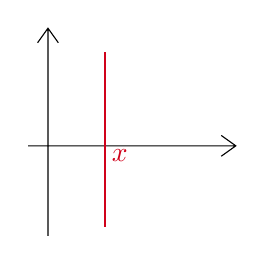
\begin{tikzpicture}[x = 0.75pt, y = 0.75pt, yscale = - 1, xscale = 1]
%uncomment if require: \path (0, 113); %set diagram left start at 0, and has height of 113

%Shape: Axis 2D [id: dp6665420354493967]
\draw (251, 63.66) - - (351, 63.66)(260.5, 7) - - (260.5, 107) (344, 58.66) - - (351, 63.66) - - (344, 68.66) (255.5, 14) - - (260.5, 7) - - (265.5, 14);
%Straight Lines [id: da4009061220418899]
\draw [color = {rgb, 255: red, 208; green, 2; blue, 27}, draw opacity = 1] (288, 18.66) - - (288, 103);

% Text Node
\draw (290, 64.23) node [anchor = north west][inner sep = 0.75pt] [color = {rgb, 255: red, 208; green, 2; blue, 27}, opacity = 1] {$x$};

\end{tikzpicture}
\end{figure}
\FloatBarrier

E possiamo allora scrivere l'antitrasformata come
\begin{equation*}
\boxed{u(x) = \frac{1}{2\pi}\int_{\Gamma_{x}} e^{zx} f(z) \dz}
\end{equation*}

\section{Convoluzione}

Ricordiamo la convoluzione di due funzioni $f, g\in L^{1}$
\begin{equation*}
(f*g)(x) = \int_{\RR} f(x - t) g(t) \dt
\end{equation*}
Con Fourier abbiamo, utile in entrambi i versi,
\begin{equation*}
\Fc(f*g, z) = \hat{f}(z)\hat{g}(z)
\end{equation*}
Per Laplace abbiamo le seguenti richieste sulle funzioni affinché siano $\Lc$ - trasformabili
\begin{itemize}
\item $f, g\in L^{1}_{\loc}$
\item $\supp f\subset [0, + \infty), \ \supp g\subset [0, + \infty)$
\item $\exists \lambda_{1}, \lambda_{2} \ \implies \ e^{- \lambda_{1} x} f(x) \in L^{1}(\RR), \ e^{- \lambda_{2} x} g(x) \in L^{1}(\RR)$
\end{itemize}
\begin{thm}
La convoluzione di due funzioni trasformabili secondo Laplace, è trasformabile secondo Laplace.
\end{thm}
\begin{proof}
\begin{equation*}
(f*g)(x) = \int_{\RR} f(x - t) g(t) \dt = \int^{x}_{0} f(x - t) g(t) \dt
\end{equation*}
$f(x - t) = 0$ se $x - t < 0$, quindi se $t > x$. Mentre $g(t) = 0$ se $t < 0$. Allora esiste l'integrale.
\begin{align*}
e^{- \lambda x}(f*g)(x) & = e^{- \lambda x}\int^{x}_{0} f(x - t) g(t) \dt\\
 & = \int^{x}_{0} e^{- \lambda (x - t)} f(x - t) e^{- \lambda t} g(t) \dt\\
 & = \left(e^{- \lambda x} f(x)\right) *\left(e^{- \lambda x} g(x)\right) \ \ \ \ \lambda \geq \max(\lambda (f), \lambda (g)) \ \implies \ \in L^{1}
\end{align*}
Soddisfa i requisiti, calcoliamone l'espressione
\begin{align*}
\Lc((f*g), s) & = \int_{\RR} e^{- sx}\left(\int_{\RR} f(x - t) g(t) \dt\right) \dx\\
 & = \iint_{\RR^{2}} e^{- s(x - t)} e^{- st} f(x - t) g(t) \dt\dx\\
 & = \int_{\RR} e^{- s(x - t)} f(x - t)\int_{\RR} e^{- st} g(t) \dt\dx = (\star)
\end{align*}
cambiamo la variabile $x' = x - t$
\begin{gather*}
(\star) = \left[\int_{\RR} e^{- sx'} f(x') \dx'\right]\left[\int_{\RR} e^{- st} g(t) \dt\right] = \Lc(f) \cdot \Lc(g)
\end{gather*}
\end{proof}


\section{Trasformata di Laplace ed equazioni differenziali}

Con Laplace risolviamo cose del tipo
\begin{equation*}
\begin{cases}
a_{n} y^{(n)}(t) + a_{n - 1} y^{(n - 1)}(t) + \cdots + a_{0} y(t) = f(t)\\
y^{(n - 1)}(0) = \textcolor[rgb]{0.82, 0.01, 0.11}{y}\textcolor[rgb]{0.82, 0.01, 0.11}{_{n - 1}}\\
\vdots \\
y(0) = \textcolor[rgb]{0.29, 0.56, 0.89}{y}\textcolor[rgb]{0.29, 0.56, 0.89}{_{0}}
\end{cases}
\end{equation*}
Trasformiamo
\begin{align*}
\Lc(y'(t), s) & = s\Lc(y(t), s) - y(0)\\
\Lc(y''(t), s) & = s\Lc(y'(t), s) - y'(0)\\
 & = s[s\Lc(y(t), s) - y(0)] - y'(0)\\
 & = s^{2}\Lc(y(t), s) - sy(0) - y'(0)\\
\Lc\left(y^{(n)}(t), s\right) & = s^{n}\Lc(y(t), s) - s^{n - 1}\textcolor[rgb]{0.29, 0.56, 0.89}{y}\textcolor[rgb]{0.29, 0.56, 0.89}{(}\textcolor[rgb]{0.29, 0.56, 0.89}{0}\textcolor[rgb]{0.29, 0.56, 0.89}{)} - s^{n - 1} y'(0) - \cdots - \textcolor[rgb]{0.82, 0.01, 0.11}{y}\textcolor[rgb]{0.82, 0.01, 0.11}{^{(n - 1)}}\textcolor[rgb]{0.82, 0.01, 0.11}{(}\textcolor[rgb]{0.82, 0.01, 0.11}{0}\textcolor[rgb]{0.82, 0.01, 0.11}{)}
\end{align*}
Per capire meglio vediamo un esmepio del secondo ordine:
\begin{equation*}
\begin{cases}
a_{2} y''(y) + a_{1} y'(t) + a_{0} y(t) = f(t)\\
y(0) = y_{0}\\
y'(0) = y_{1}
\end{cases}
\end{equation*}
Ora trasformiamo
\begin{gather*}
a_{2}\left(s^{2}\Lc(y(t), s) - sy_{0} - y_{1}\right) + a_{1}(s\Lc(y(t), s) - y_{0}) + a_{0}\Lc(y(t), s) = \Lc(f(t), s)\\
\left(a_{2} s^{2} + a_{1} s + a_{0}\right)\Lc(y(t), s)\underbrace{- a_{2}(sy_{0} + y_{1}) - a_{1} y_{0}}_{\text{polinomio in} \ s}  = \Lc(f(t), s)
\end{gather*}
Otteniamo quindi
\begin{equation*}
\Lc(y(t), s) = \frac{\Lc(f(t), s) + a_{2}(sy_{0} + y_{1}) + a_{1} y_{0}}{a_{2} s^{2} + a_{1} s + a_{0}}
\end{equation*}
che ci permette di introdurre in maniera naturale anche i dati iniziali:
\begin{equation*}
y(t) = f(t) *\Lc^{- 1}\left(\frac{1}{a_{2} s^{2} + a_{1} s + a_{0}}, t\right) + \Lc^{- 1}\left(\frac{a_{2}(sy_{0} + y_{1}) + a_{1} y_{0}}{a_{2} s^{2} + a_{1} s + a_{0}}, t\right)
\end{equation*}
e allora
\begin{equation*}
\frac{1}{s - s_{0}} + \frac{1}{s - s_{1}} + \cdots \ \ \ \ \Lc\left(e^{\alpha t} H(t), s\right) = \frac{1}{s - \alpha}\ .
\end{equation*}